%设置页面边距(word标准页面)
\documentclass[a4paper]{article}
\usepackage{geometry}
\geometry{a4paper,left=2.7cm,right=2.7cm,top=2.54cm,bottom=2.54cm}
\usepackage{tikz}
\usetikzlibrary{shapes.geometric, arrows}
\usepackage{wrapfig}

%导入ctex包
\usepackage[UTF8,heading=true]{ctex}
\tikzset{
    startstop/.style={
        rectangle,
        rounded corners,
        minimum width=3cm,
        minimum height=1cm,
        text centered,
        draw=black,
        fill=red!30
    },
    io/.style={
        trapezium,
        trapezium left angle=70,
        trapezium right angle=110,
        minimum width=3cm,
        minimum height=1cm,
        text centered,
        draw=black,
        fill=blue!30
    },
    process/.style={
        rectangle,
        minimum width=3cm,
        minimum height=1cm,
        text centered,
        draw=black,
        fill=orange!30
    },
    decision/.style={
        diamond,
        aspect=2, % 控制菱形的宽高比
        minimum width=3cm,
        minimum height=1cm,
        text centered,
        draw=black,
        fill=green!30
    },
    arrow/.style={
        thick,
        -Stealth % 使用Stealth箭头样式
    }
}

%设置摘要格式
\usepackage{abstract}
\setlength{\abstitleskip}{0em}
\setlength{\absleftindent}{0pt}
\setlength{\absrightindent}{0pt}
\setlength{\absparsep}{0em}
\renewcommand{\abstractname}{\textbf{\zihao{4}{摘要}}}
\renewcommand{\abstracttextfont}{\zihao{-4}} %设置摘要正文字号

%设置页眉和页脚,只显示页脚居中页码
\usepackage{fancyhdr}
\pagestyle{plain}

%调用数学公式包
\usepackage{amssymb}
\usepackage{amsmath}

%调用浮动包
\usepackage{float}
\usepackage{subfig}
\captionsetup[figure]{labelsep=space} %去除图标题的冒号
\captionsetup[table]{labelsep=space} %去除表格标题的冒号
%设置标题格式
\ctexset {
	%设置一级标题的格式
	section = {
		name={,、},
		number=\chinese{section}, %设置中文版的标题
		aftername=,
	},
	%设置三级标题的格式
	subsubsection = {
		format += \zihao{-4} % 设置三级标题的字号
	}
}


%使得英文字体都为Time NewTown
%\usepackage{times}

%图片包导入
\usepackage{graphicx}
\graphicspath{{figures/}} %图片在当前目录下的figures目录

%参考文献包引入
\usepackage{cite}
\usepackage[numbers,sort&compress]{natbib}

%代码格式
\usepackage{listings}
\usepackage{graphicx}%写入python代码
\usepackage{pythonhighlight}%python代码高亮显示
\lstset{
	%numbers=left, %设置行号位置
	%	numberstyle=\tiny, %设置行号大小
	keywordstyle=\color{blue}, %设置关键字颜色
	commentstyle=\color[cmyk]{1,0,1,0}, %设置注释颜色
	escapeinside=``, %逃逸字符(1左面的键),用于显示中文
	breaklines, %自动折行
	extendedchars=false, %解决代码跨页时,章节标题,页眉等汉字不显示的问题
	xleftmargin=1em,xrightmargin=1em, aboveskip=1em, %设置边距
	tabsize=4, %设置tab空格数
	showspaces=false %不显示空格
}


\renewcommand{\refname}{}

%item包
\usepackage{enumitem}

%表格加粗
\usepackage{booktabs}

%设置表格间距
\usepackage{caption}

%允许表格长跨页
\usepackage{longtable}

%伪代码用到的宏包
\usepackage{algorithmic}
\usepackage{algorithm}

\usepackage{accents}

%正文区
\title{“板凳龙” 运动系统的建模与优化}
\date{} %不显示日期

%文档
\begin{document}
	\maketitle
	\vspace{-6em} %设置摘要与标题的间距
	\zihao{-4} %设置正文字号
	%摘要部分
	\begin{abstract}
		“板凳龙”是浙闽地区的传统民俗活动,其舞龙队能够将上百条板凳螺旋式盘绕形成巨龙。在舞龙过程中,舞龙队应保持较小的间距和较快的行进速度;在题设要求下,通过对“板凳龙”问题的进行分析与适当建模,我们给出了所有指定时刻把手的坐标和速度,在等距螺线下求出了板凳龙的最小螺距和最大速度。

		\hspace{0.2em}\textbf{针对问题一},以等距螺线为中心建立了\textbf{极坐标系},用\textbf{参数方程}刻画舞龙队的行进位置和速度。首先,建立等距螺线和龙头速度间关系的\textbf{微分方程模型},利用\textbf{积分法}求解出了\textbf{舞龙队龙头的坐标关于行进时间的解析式};然后,基于已知的把手位置,建立了舞龙队伍的\textbf{几何模型},通过不断对后一把手进行\textbf{二分查找},\textbf{迭代}查找确定了舞龙队所有把手的坐标;接着,用\textbf{微分方程转化为差分方程}的\textbf{微元法},得到了舞龙队在各个位置下的速度。

		\textbf{针对问题二},建立了以舞龙队\textbf{最长运动时间}为\textbf{决策变量和目标函数}的\textbf{复杂单目标优化模型}。针对板凳不能碰撞的约束条件,使用\textbf{构造凸集与向量代数方法}将其转化为\textbf{线段相交}约束,用\textbf{跨立实验}判断是否相交;接着提出了适用于本模型的\textbf{拟粒子群算法}求解出优化结果,得到了从起始位置开始舞龙队最多可以前进\textbf{412.474213s}。通过可视化和灵敏度分析对模型进行了验证。最后完成了位置和速度的求解。

		\textbf{针对问题三},建立了以\textbf{等距螺线螺距}为\textbf{目标函数}的\textbf{单目标优化模型}。使用了问题二建立的模型和算法,求解出特定螺距下龙头与原点的\textbf{最小距离}。通过\textbf{可视化与回归分析}确认了螺距-龙头与原点最小距离函数的\textbf{单调性}。最后利用\textbf{二分查找}求解出满足题目要求的最小螺距为\textbf{46.269531cm}。

		\textbf{针对问题四},首先,\textbf{严格按照问题要求的全体约束条件}计算出了舞龙队盘入路线、盘出路线和掉头路线的圆弧位置,利用\textbf{解析几何}的方法确定了舞龙队的\textbf{掉头路线方程},\textbf{确认了在约束条件下圆弧位置固定因而不可优化}。然后,取\textbf{时间作为参数},建立了舞龙队\textbf{行进路线的参数方程}。最后,利用\textbf{二分查找算法}和\textbf{微元法},计算出了舞龙队各把手在各个时刻下的位置和速度的数值解。

		\textbf{针对问题五},首先,通过建立\textbf{运动曲线几何模型},得到把手间的\textbf{速度大小和螺线轨迹曲率的关系},进而确定把手速度最大值的分布规律% TODO
		。然后,建立以把手全局最大速度为目标函数的单目标优化模型,绘制出\textbf{最大速度-时间分布图}%TODO
		。最后,利用\textbf{模拟退火算法},求解出\textbf{最大速度把手的时空位置},将最大速度与龙头速度在\textbf{时间尺度下进行缩放}%TODO
		使得满足题设要求,解得满足题意的龙头\textbf{最大速度为 1.246267m/s}。  \\
		%关键词(上文最后一段要用“\\”换行)
		\newline
		\noindent{\textbf{关键词:} \textbf{微分方程}\quad   \textbf{微元法}\quad \textbf{粒子群算法} \quad \textbf{单目标优化模型}\quad \textbf{模拟退火算法}}
	\end{abstract}

	\clearpage %换页

	%正文部分
	%Part one
	\section{问题背景与重述}
	\subsection{问题背景}
	“板凳龙”是浙闽地区的传统民俗活动,其舞龙队能够将上百条板凳螺旋式盘绕形成巨龙。舞龙队的盘绕路线大致呈螺线状向内部盘绕。其中,螺距的最小化与速度的最大化不仅影响舞龙队形的紧凑度和动态美,也直接关系到表演的安全性。通过对这些参数的深入研究,可以优化舞龙表演的编排,确保参与者的安全,为传统文化的传承与发展提供科学支撑。

	%\begin{figure}[H]
	%	\centering %图片居中
	%	\captionsetup{skip=4pt} % 设置标题与表格的间距为4pt
	%	\includegraphics[width=10cm]{图片文件名} %width设置图片大小
	%	\caption{商超蔬菜示意图\label{商超蔬菜示意图}} %设置图片的标题及引用标签
	%\end{figure}

	\subsection{问题重述}
		\textbf{问题一:}在题目给定的 55cm 螺距的等距螺线作为行进路线的情形下,取龙头位置为第十六圈与 x 轴交点处为龙头的初始位置,且龙头以 1m/s 的速度向内顺时针盘绕,计算 0-300s 内每隔一秒舞龙队各把手的所在位置以及速度。

		\textbf{问题二:}在题目给定的 55cm 螺距的等距螺线作为行进路线的情形下,取龙头位置为第十六圈与 x 轴交点处为龙头的初始位置,且龙头以 1m/s 的速度向内顺时针盘绕。求解板凳间首次发生碰撞的时刻,进一步求解该时刻各个把手的位置坐标和速度。

		\textbf{问题三:}优化等距螺线的螺距,使得舞龙队首次发生碰撞的位置位于以等距螺线中心为圆心,9m为直径的圆的外部。在此约束条件下求等距螺线螺距的最小值。

		\textbf{问题四:}在题目给定的掉头路线的基础上,试寻找符合要求的掉头路线使路线长度更短。同时,在题目指定的掉头路线基础上,求解舞龙队各把手在 -100s 到 100s 内每一秒的位置和速度。

		\textbf{问题五:}在问题四的设定路线上,确定龙头行进的最大速度,使得每一把手的行进速度都不超过 2m/s

	%Part Two
	\section{问题分析}
	\subsection{问题一的分析}
		问题一要求我们在给定情景下分析从初始时刻到 300s 为止的时间中舞龙队各把手的中心位置和速度。首先,需要推导出了描述等距螺线路径与速度关系的微分方程,并解出了龙头位置与行进时间的函数关系。接着,需要利用已知的把手位置,采用了二分查找算法,迭代地确定了舞龙队所有把手的具体物理位置,从而计算出每一把手在不同时间点的位置。然后,需要应用微元法分析了舞龙队各把手的位置变化,从而得出了它们的速度。
	\subsection{问题二的分析}
        问题二要求我们确定板凳之间首次发生碰撞时各个把手的位置和速度。由于问题一模型的建立,已经建立了映射关系$t\to<pos_i,v_i>$。因此只需要计算板凳发生碰撞的最小时间。该问题可分解为两个小问题,首先是\textbf{给定所有点的位置格局,板凳是否碰撞的判定问题},使用了向量代数和几何方法给出了判定,该问题的解答给出了优化模型的约束条件;其次是\textbf{搜索满足板凳碰撞约束条件的最小速度的优化问题}。结合满足约束条件的t在实数域内为\textbf{多个}连续区间这一特征,难以遍历搜索得到最小值,可以借鉴\textbf{多个}粒子分别搜索的\textbf{粒子群算法},通过一定改造得到了本问题的求解方法。
	\subsection{问题三的分析}
        问题三要求我们找到最小的螺距,使得板凳龙首次碰撞时,龙头前把手位于中央半径为4.5m的圆内部。我们建立了\textbf{以螺距为决策目标、首次碰撞时龙头距离圆心长度小于4.5m为约束条件的单目标优化模型}。试探性地使用问题二中的求解方法计算出了不同螺距下板凳龙龙头距离原点的最小长度,通过可视化分析,得到最小长度与螺距呈现\textbf{单调的函数关系}。因此,直接采用\textbf{二分查找的算法得到螺距的最小值}。并通过可视化的运动系统验证了模型。
	\subsection{问题四的分析}
		问题四要求我们确定在给定行进路线下的舞龙队各把手在给定时间下的位置和行进速度。首先,需要计算出掉头范围内两圆弧的圆心和半径,以及盘入螺线和盘出螺线的方程。然后,综合分析两圆弧和盘入盘出等距螺线,\textbf{建立舞龙队行进路线的参数方程}。最后,利用\textbf{二分查找算法迭代}确定每个把手的位置,再利用微元法计算出把手速度的数值解。
	\subsection{问题五的分析}
		问题五要求在问题四的设定路线上,求解龙头的最大速度使得每个把手的速度在任一时刻都不超过 2m/s。由于各个把手依托“板凳龙”构成\textbf{速度关联模型},\textbf{只需要求解给定龙头速度下把手的最大速度},再沿时间对龙头速度进行缩放即可得到最大龙头速度。因此,首先根据\textbf{曲线下速度关联的几何性质},确定\textbf{最大速度的时间分布规律},将优化目标函数降为一元函数。然后根据得到的目标函数,进一步\textbf{缩小最大值的查找范围}。接着,利用\textbf{模拟退火算法}、\textbf{三分算法}求得速度最大值。最后,对龙头速度进行等比例\textbf{缩放},即可得到满足题意要求的最大龙头速度

	%Part Three
	\section{模型假设}
	%假设的列表
	\begin{enumerate}
		\item 假设板凳龙盘入与盘出时,龙头、各节龙身以及龙尾之间连接牢固,旋转润滑,运动连续不停顿。
		\item 假设不考虑板凳厚度对板凳龙整体运动产生的影响。
		\item 假设板凳龙的各板凳均位于同一平面上,不考虑板凳间搭接导致的板凳高度起伏,不考虑地面的高度起伏。
        \item 假设运动模型中所有被纳入考虑的位置均空旷,不存在障碍物阻挡或不可到达的区域。
        \item 在建立碰撞模型时,不考虑举板凳的人所占据的空间,假设舞龙队发生碰撞当且仅当板凳发生碰撞。
	\end{enumerate}

	%Part Four
	\section{符号说明}
	%浮动体表格,使用table实现
	\begin{table}[H] %[h]表示在此处添加浮动体,默认为tbf,即页面顶部、底部和空白处添加
		\captionsetup{skip=4pt} % 设置标题与表格的间距为4pt
		\centering
		\setlength{\arrayrulewidth}{2pt} % 设置表格线条宽度为1pt
		\begin{tabular}{cc} %c表示居中,l表示左对齐,r表示右对齐,中间添加“|”表示竖线
			\hline
			\makebox[0.15\textwidth][c]{符号} & \makebox[0.6\textwidth][c]{说明}  \\
			\hline
			$\rho$ & 极坐标下点的模长  \\
			$\theta$ & 极坐标下点的辐角  \\
			$D$ & 等距螺线螺距  \\
			$L_1$ & 龙头板凳长  \\
			$L_2$ & 龙身龙尾板凳长  \\
			$d$ & 板凳宽  \\
			$l$ & 板凳板头长 \\
			$R$ & 掉头区域半径大小\\
			$r_1$ & 前一掉头圆弧半径\\
			$r_2$ & 后一掉头圆弧半径\\
			$t$ & 舞龙队运动时间  \\
			$A_0$ & 龙头把手的中心点  \\
			$A_i$ & 第 i 节龙身靠前把手的中心点  \\
			$A_{223}$ & 龙尾后侧把手中心点  \\
			$B_i$ & 第i结龙身行进方向右前方端点 \\
			$B_i'$ &  第i结龙身行进方向后方端点 \\
			$C_i$ & 第i结龙身行进方向左前方端点 \\
			$C_i'$ & 第i结龙身行进方向左后方端点 \\
			$B$ & 掉头曲线起始位置 \\
			$B'$ & 掉头曲线结束位置 \\
			$l_B$ & 掉头曲线起始位置切线 \\
			\hline
		\end{tabular}
		% \hline是横线,采用\makebox设置列宽
	\end{table}


	%Part Five
	\section{模型的建立与求解}
	\subsection{问题一模型的建立与求解}
	\subsubsection{龙头把手与其余把手的位置的几何递推模型与求解}

		依据题意,舞龙队的行进路线由 $D = 55cm$ 的等距螺线确定。选用极坐标刻画行进路线时,该路线可以由以下方程确定:

		\begin{equation}
			\rho = \frac{D}{2\pi}\theta, \quad \theta \in [0,+\infty)
		\end{equation}

		使用形如 $(\rho, \theta)$ 的方式表示点的坐标,因此初始点 A 点的坐标可以表示为 $( 16 \cdot 0.55, 16 \cdot 2\pi )$。

		题设给定的初始条件中,只有龙头把手的位置是已知信息,因此需要得到龙头把手的位置和其余所有把手的位置关系才能确定其余把手的位置。通过解析可以发现:该关系难以求出解析解。因此可以考虑\textbf{从龙头把手位置逐级递推到每一把手的位置}。

		为了做到这一点,考虑到对给定的前一把手位置($\theta_{i}$),当$\Delta \theta > \frac{\pi}{2}$时,$\Delta l$关于$\Delta \theta$递增,故我们选用了二分查找算法,在任一把手 $A_i$ 位置已知的情况下,查找下一把手所在位置。即给定 $\theta_{i}$ ,确定 $\theta_{i+1}$ 的大小。而 $\theta_{i+1}$ 合适当且仅当两把手的间距正好等于板凳两孔中心的距离。根据极坐标下的余弦定理,两点间的位置即为:

		$$\Delta l = \sqrt{\rho_i^2 + \rho_{i+1}^2 - 2\rho_i \rho_{i+1} \cos(\theta_i - \theta_{i+1})}$$

		代入 $\rho$ 并令 $\Delta l$ 分别减去龙头和龙身除去板头的长度,即分别减去 $L_1 - 2 \cdot l$ 和 $L_2 - 2 \cdot l$,即可得到二分查找的目标函数 $f$ ,其零点即为 $\theta_{i+1}$ 的二分查找值:

		\begin{equation}
			f(\theta) = \frac{D}{2\pi} \sqrt{\theta^2 + \theta_i^2 - 2\theta \theta_i \cos(\theta - \theta_i)} - (L_j - 2l), \quad j=1, 2
		\end{equation}

		目标函数 $f$ 二分查找所得的零点即为 $\theta_{i+1}$ 的数值解。

		二分求解代码见附录 2 calculate.py 文件。将计算得到的位置绘制在直角坐标中大致如图%TODO
		所示
		
		\begin{figure}[H]
			\centering
			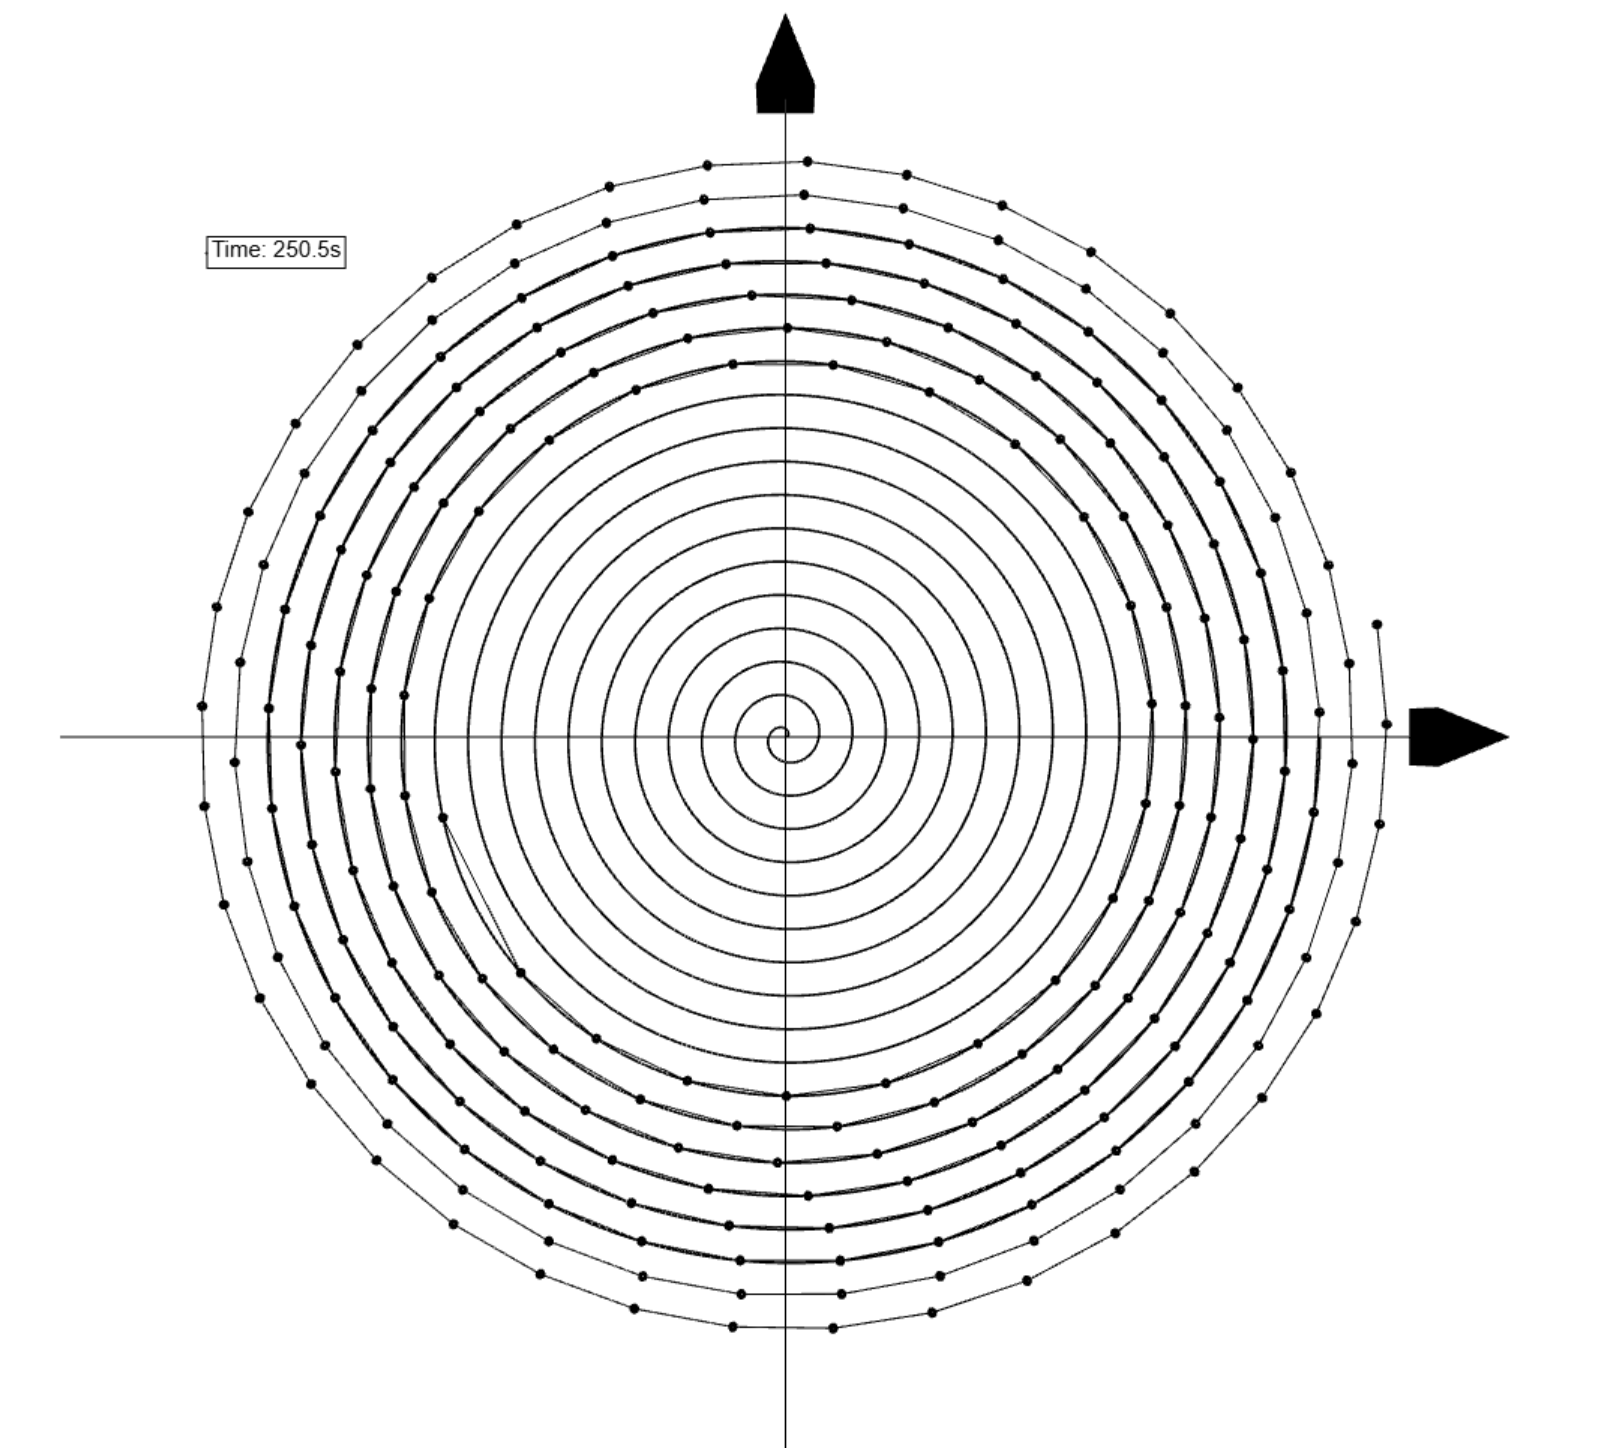
\includegraphics[width=0.5\linewidth]{image/Figure_5111.png}
			\caption{问题一把手位置}
			\label{Figure_5111}
		\end{figure}

	\subsubsection{龙头把手的位置与时间关系的常微分方程模型与求解}

		5.1.1 小节提供了由龙头把手计算其余各个把手位置的方法,因此只需要确定每一秒龙头把手的位置,利用上一小节的方法,即可得到每一秒钟各个把手的位置信息。

		极坐标下,龙头把手位置可以由 $\theta$ 参数唯一确定。因此,只需要求解出龙头的辐角 $\theta$ 与时间 $t$ 的关系即可。对等距螺线使用微元法,可以用 $d\theta$ 和 $d\rho$ 表示出螺线弧微元 $ds$:

		$$ ds = \sqrt{(d\rho)^2 + (\rho d\theta) ^ 2}$$

		而微元 $ds$ 等于龙头在 $dt$ 时间内行进的距离,即:

		\begin{equation}
			\sqrt{(d\rho)^2 + (\rho d\theta) ^ 2} = vdt
		\end{equation}

		联立 (1) 和 (3) 式消去 $\rho$,用\textbf{分离变量法}求解\textbf{常微分方程}即可解得龙头的辐角 $\theta$ 和时间 $t$ 满足以下关系:

		\begin{equation}
			g(\theta) = \frac{D}{2\pi}(-\frac{1}{2}\ln(\sqrt{\theta^2+1}-\theta)+\frac{1}{2}\theta\sqrt{\theta^2+1})=vt+C
		\end{equation}

		% TODO 常数 C 需要进一步计算

		带入初值条件$$g(32  \pi) = C$$,利用数值计算即可求得给定时刻下龙头把手的位置。

	\subsubsection{各把手的速度的差分方程模型与求解}

		5.1.2 小节计算出了各个把手的位置在给定时刻下的数值解,而速度是位置在时间尺度下的微元。因此,只需要取时间微元 $\Delta t$ ,并计算在给定时间 $t_1$ 两侧的 $\Delta t$ 下的把手位置的位移模长 $|\vec{x}(t_1+\Delta t) - \vec{x}(t_1 - \Delta t)|$ ,将其除以两倍的 $\Delta t$ 即可得到速度大小。



		具体来说,对于给定的时间 $t_1$ ,把手 $A_i$ 此时的速度大小的数值解为:

		\begin{equation}
			v_{t1} = \dfrac{\sqrt{(x_i(t_1 + \Delta t) - x_i(t_1 - \Delta t))^2 + (y_i(t_1 + \Delta t) - y_i(t_1 - \Delta t))^2}}{2\Delta t}
		\end{equation}		

		利用这种方式计算出问题一中的各个把手的位置和速度见 result1.xlsx 文件。其中 0 s、60 s、120 s、180 s、240 s、300 s 时,龙头前把手、龙头后面第 1、51、101、151、201 节龙身前把手和龙尾后把手的位置和速度如下表所示:


		\begin{table}[H] %[h]表示在此处添加浮动体,默认为tbf,即页面顶部、底部和空白处添加
			\captionsetup{skip=4pt} % 设置标题与表格的间距为4pt
			\caption{问题一的位置结果}
			\centering
			\setlength{\arrayrulewidth}{0.5pt} % 设置表格线条宽度为1pt
			\begin{tabular}{|c|c|c|c|c|c|c|} %c表示居中,l表示左对齐,r表示右对齐,中间添加“|”表示竖线
				\hline
				% \makebox[0.15\textwidth][c]{符号} & \makebox[0.6\textwidth][c]{说明}  \\
				% \hline
				& 0 s & 60 s & 120 s & 180 s & 240 s & 300 s \\ \hline
				龙头 x (m)         & 8.800000 &	5.799209 &	-4.084887 &	-2.963609 &	-0.818702 &	4.420274 \\ \hline
				龙头 y (m)         & -0.000000 &	-5.771092 &	-6.304479 &	6.094780 &	5.590600 &	2.320429 \\ \hline
				第 1 节龙身 x (m)  & 8.363824 &	7.456758 &	-1.445473 &	-5.237118 &	-3.469210 &	2.459489 \\ \hline
				第 1 节龙身 y (m)  & 2.826544 &	-3.440399 &	-7.405883 &	4.359627 &	4.516167 &	4.402476 \\ \hline
				第 51 节龙身 x (m) & -9.518732 &	-8.686317 &	-5.543150 &	2.890455 &	-6.560125 &	-6.301346 \\ \hline
				第 51 节龙身 y (m) & 1.341137 &	2.540108 &	6.377946 &	7.249289 &	1.969759 &	0.465829 \\ \hline
				第 101 节龙身 x (m) &2.913983 &	5.687116 &	5.361939 &	1.898794 &	0.218823 &	-6.237722 \\ \hline
				第 101 节龙身 y (m) &-9.918311 &	-8.001384 &	-7.557638 &	-8.471614 &	7.831999 &	3.936008 \\ \hline
				第 151 节龙身 x (m) &10.861726 &	6.682311 &	2.388757 &	1.005154 &	4.451294 &	7.040740 \\ \hline
				第 151 节龙身 y (m) &1.828753 &	8.134544 &	9.727411 &	9.424751 &	-7.486030 &	4.393013 \\ \hline
				第 201 节龙身 x (m) &4.555102 &	-6.619664 &	-10.627211 &	-9.287720 &	-1.731014 &	-7.458662 \\ \hline
				第 201 节龙身 y (m) &10.725118 &	9.025570 &	1.359847 &	-4.246673 &	9.344557 &	-5.263384 \\ \hline
				龙尾(后) x (m)    &-5.305444 &	7.364557 &	10.974348 &	7.383896 &	7.057739 &	1.785033 \\ \hline
				龙尾(后) y (m)    &-10.676584 &	-8.797992 &	0.843473 &	7.492370 &	-6.846021 &	9.301164 \\ \hline
			\end{tabular}
			% \hline是横线,采用\makebox设置列宽
		\end{table}

		\begin{table}[H] %[h]表示在此处添加浮动体,默认为tbf,即页面顶部、底部和空白处添加
		\captionsetup{skip=4pt} % 设置标题与表格的间距为4pt
		\caption{问题一的速度结果}
		\centering
		\setlength{\arrayrulewidth}{0.5pt} % 设置表格线条宽度为1pt
		\begin{tabular}{|c|c|c|c|c|c|c|} %c表示居中,l表示左对齐,r表示右对齐,中间添加“|”表示竖线
			\hline
			% \makebox[0.15\textwidth][c]{符号} & \makebox[0.6\textwidth][c]{说明}  \\
			% \hline
			& 0 s & 60 s & 120 s & 180 s & 240 s & 300 s \\ \hline
			龙头 (m/s)      &    1.000000 &	1.000000 &	1.000000 &	1.000000 &	1.000000 &	1.000000 \\ \hline
			第 1 节龙身 (m/s) &  0.999971 &	0.999961 &	0.999945 &	0.999917 &	0.999859 &	0.999709 \\ \hline
			第 51 节龙身 (m/s) & 0.999742 &	0.999662 &	0.999540 &	0.999331 &	0.998940 &	0.998064 \\ \hline
			第 101 节龙身 (m/s) &0.999575 &	0.999455 &	0.999277 &	0.998971 &	0.998436 &	0.997302 \\ \hline
			第 151 节龙身 (m/s) &0.999451 &	0.999303 &	0.999082 &	0.998726 &	0.998121 &	0.996860 \\ \hline
			第 201 节龙身 (m/s) &0.999352 &	0.999190 &	0.998942 &	0.998552 &	0.997902 &	0.996575 \\ \hline
			龙尾(后) (m/s) &   0.999317 &	0.999143 &	0.998889 &	0.998490 &	0.997827 &	0.996476 \\ \hline
		\end{tabular}
		% \hline是横线,采用\makebox设置列宽
		\end{table}
		
		\subsubsection{模型灵敏度验证}
		
		取速度作为因变量。随把手编号的增大,把手速度随之发生变化。第 100s 下的速度关于把手编号的函数图像如图%TODO
		所示。
		
		\begin{figure}[H]
			\centering
			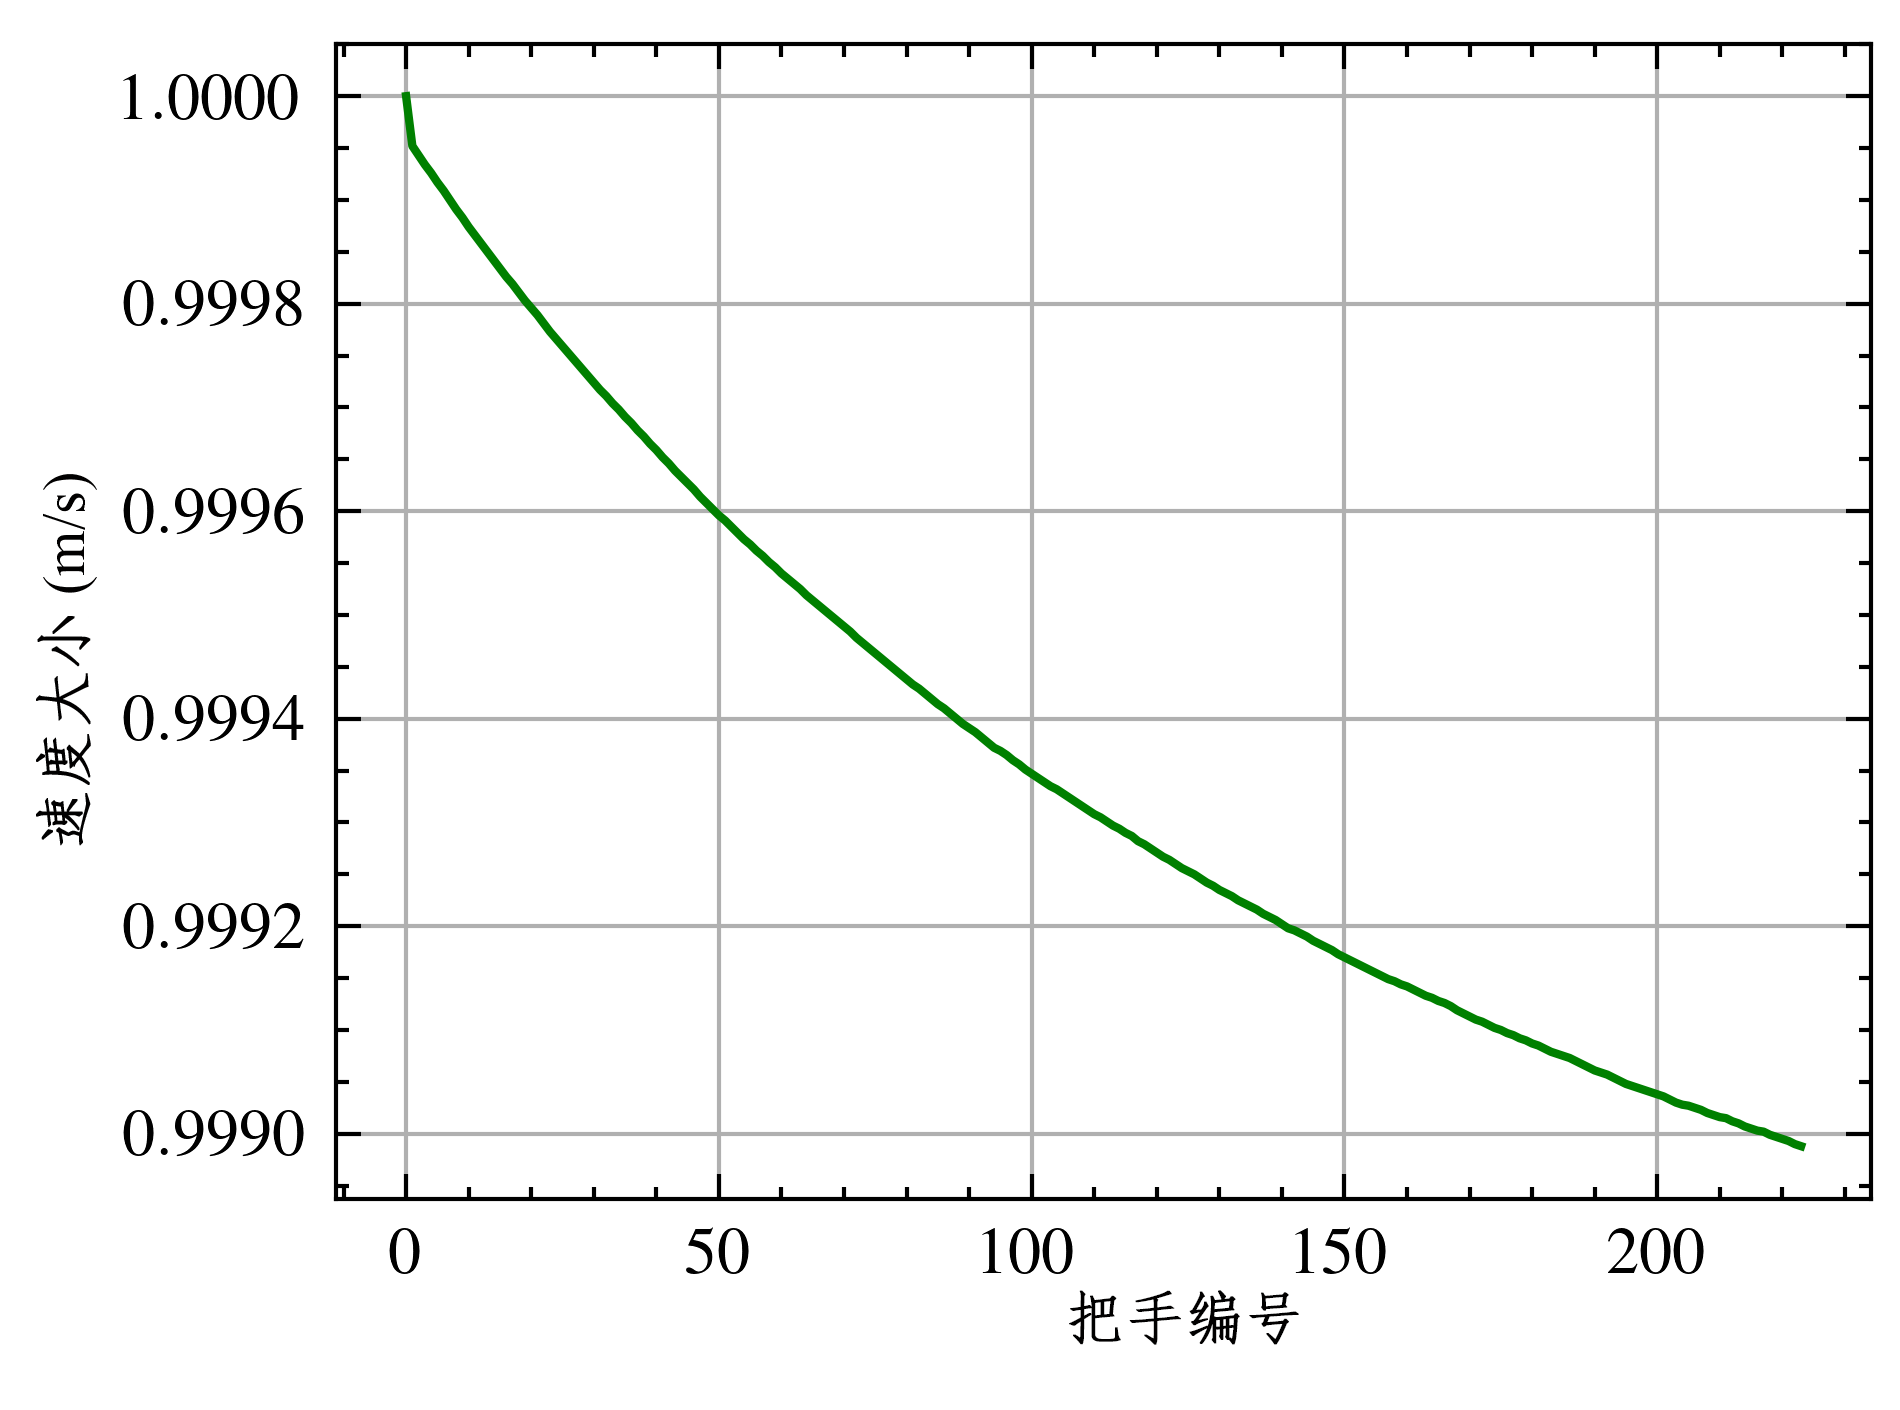
\includegraphics[width=0.5\linewidth]{image/Figure_5131.png}
			\caption{100s 下把手速度随把手编号的分布}
			\label{Figure_5131}
		\end{figure}
		
		调整把手编号,比对各把手的速度可知:随着把手编号增大,把手的行进速度逐渐稳定单调降低,进而说明构建模型的灵敏性较高。此外,据此可发现龙头的速度略高于龙尾速度。这位问题五分析最大速度提供了数据支撑

	\subsection{问题二模型的建立与求解}
	     针对问题二,我们建立了以板凳龙运动的最长时间为决策变量和目标函数,以板凳间不互相碰撞为约束条件的\textbf{最优化模型}。通过\textbf{构造凸集}、\textbf{向量代数}和\textbf{计算几何}方法将约束条件转化为\textbf{跨立实验}。使用了\textbf{拟粒子群算法}对最优化问题进行启发式求解。得到了从起始位置开始舞龙队最多可以前进\textbf{412.474213s}。并使用问题一的模型求解了当前时刻各把手的位置与速度。

        \subsubsection{板凳碰撞最优化模型的建立}
    \begin{itemize}
        \item {\textbf{边界坐标的确定}}
        问题一模型确立了$t\to<pos_i,v_i>$的映射关系,故能够由时刻确定所有把手$A_{i}$位置,即$A_{i}$为t的函数,记作:$$A_{i}(t) = (x_i, y_i)$$
        \begin{figure}[H]
            \centering
            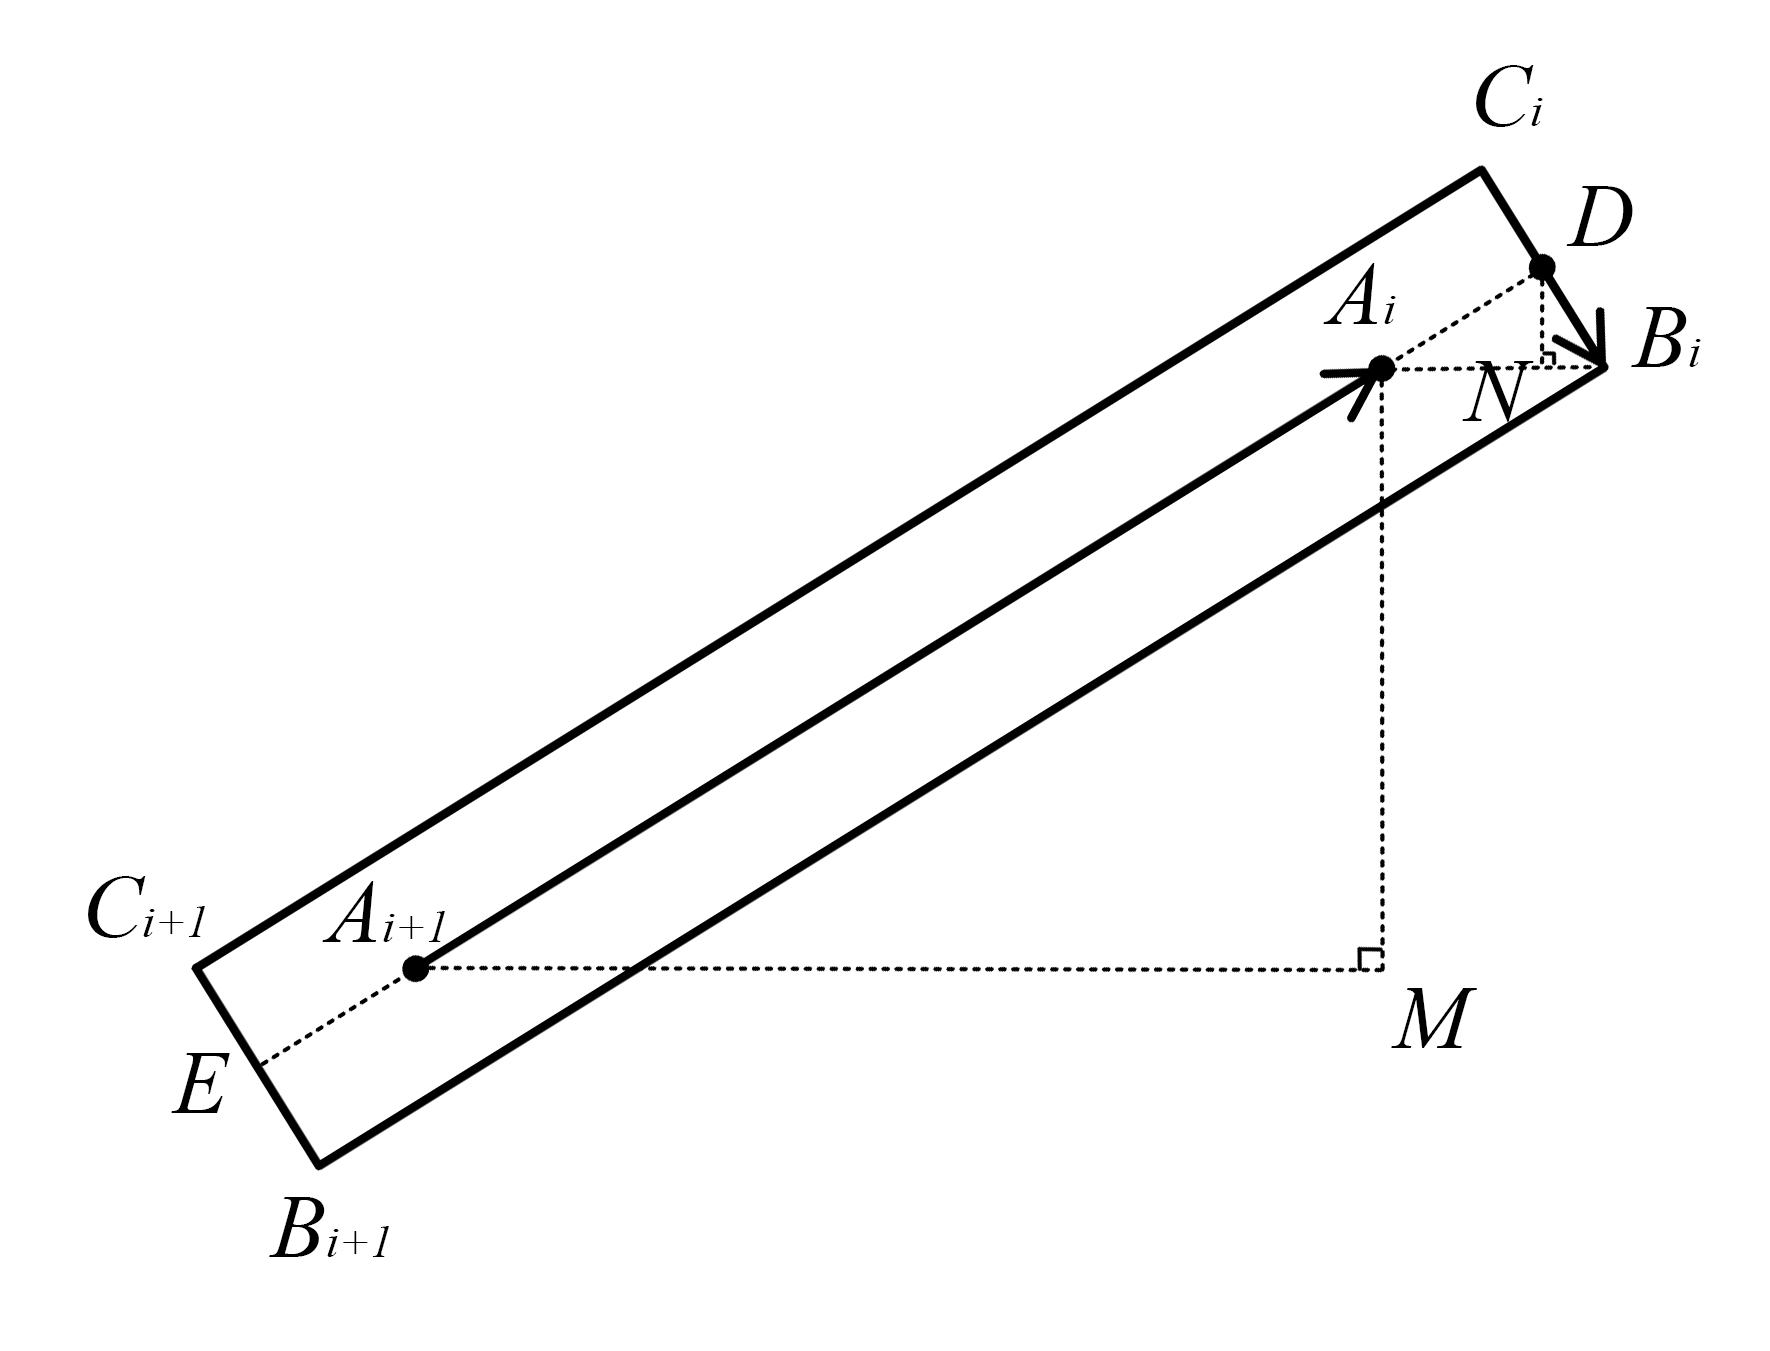
\includegraphics[width=0.5\linewidth]{image/Figure_5213.png}
            \caption{边界坐标与把手坐标关系的几何模型}
            \label{fig:enter-label1}
        \end{figure}

        下面建立向量代数模型,确定板凳四边界点同板凳把手$A_i(t)$的解析关系。如图所示,板凳前缘中央点假设为$D(x,y)$,根据向量平行关系有
        $$
                   \overrightarrow{A_iD} = \lambda\overrightarrow{A_{i+1}A_i}
        ,\quad\quad \lambda = \left\{ \begin{array}{c}
              27.5 / 286, i = 0 \\
              27.5 / 165, i > 0

        \end{array}\right.
        $$

        带入坐标可以得到$D_i = ((\lambda + 1) x_{i} - \lambda x_{i + 1}, (\lambda + 1) y_{i} - \lambda y_{i + 1})$,同理可以得到,板凳尾缘中央点$E_i = ((\lambda + 1) x_{i + 1} - \lambda x_{i}, (\lambda + 1) y_{i + 1} - \lambda y_{i})$。
        计算同中轴线垂直的向量,根据相似关系$\Delta A_{i+ 1}A_iM \sim \Delta D_iB_iN$可以求解得到
        $$\overrightarrow{D_i B_i} = (\lambda 1 (y_i - y_{i + 1}), \lambda 1 (x_{i + 1} - x_i)),
        \quad \quad \lambda 1 = \left\{ \begin{array}{c}
             15/286, i = 0  \\
             15/165, i > 0
        \end{array}
        \right.$$

         进一步可计算得到板凳的四个顶点直角坐标
         \begin{equation}
         \begin{aligned}
         \begin{split}
         B_i = ((\lambda + 1) x_{i} - \lambda x_{i + 1} + \lambda 1 (y_i - y_{i + 1}), (\lambda + 1) y_{i} - \lambda y_{i + 1} + \lambda 1 (x_{i + 1} - x_i)) \\= \phi 1(A_i, A_{i + 1})
         \end{split}
         \end{aligned}
         \end{equation}
         \begin{equation}\begin{aligned}\begin{split} B_{i}' = ((\lambda + 1) x_{i + 1} - \lambda x_{i} + \lambda 1 (y_i - y_{i + 1}), (\lambda + 1) y_{i + 1} - \lambda y_{i} + \lambda 1 (x_{i + 1} - x_i))\\ =    \phi 2(A_i, A_{i + 1})\end{split}\end{aligned}\end{equation}
         \begin{equation}\begin{aligned}\begin{split} C_i = ((\lambda + 1) x_{i} - \lambda x_{i + 1} - \lambda 1 (y_i - y_{i + 1}), (\lambda + 1) y_{i} - \lambda y_{i + 1} - \lambda 1 (x_{i + 1} - x_i))\\ = \phi 3(A_i, A_{i + 1})\end{split}\end{aligned}\end{equation}
         \begin{equation}\begin{aligned}\begin{split} C_i' = ((\lambda + 1) x_{i + 1} - \lambda x_{i} - \lambda 1 (y_i - y_{i + 1}), (\lambda + 1) y_{i + 1} - \lambda y_{i} - \lambda 1 (x_{i + 1} - x_i))\\ = \phi 4(A_i, A_{i + 1})\end{split}\end{aligned}\end{equation}
        \item {\textbf {凸集构造与线段相交模型的建立}}

         对任意一个板凳,考虑其后方除相邻板凳之外所有板凳的内侧长边围成的折线,可将折现变换为一个凸集的边界。变换方法是对把手$A_iA_{i+1}$确定的板凳,将内部长边$B_{i+2}B_{i+2}'$延长为射线,取距离$B_{i+2}'$最近的与折线的交点。板凳存在相撞的必要条件是存在板凳的外缘线段上的点,位于凸集外部。这意味着对任意板凳,若与外圈板凳若发生碰撞,必存在板凳的长边与外界凸集边界相交,又凸集边界必为某条板凳靠内长边的一部分,故存在板凳的外部长边同外侧板凳的内部长边相交。另一方面,如果存在某两条不相邻的板凳的长边存在交点,则必存在板凳碰撞。这就建立了板凳碰撞与线段相交的等价关系。
		\begin{figure}[H]
		    \centering
		    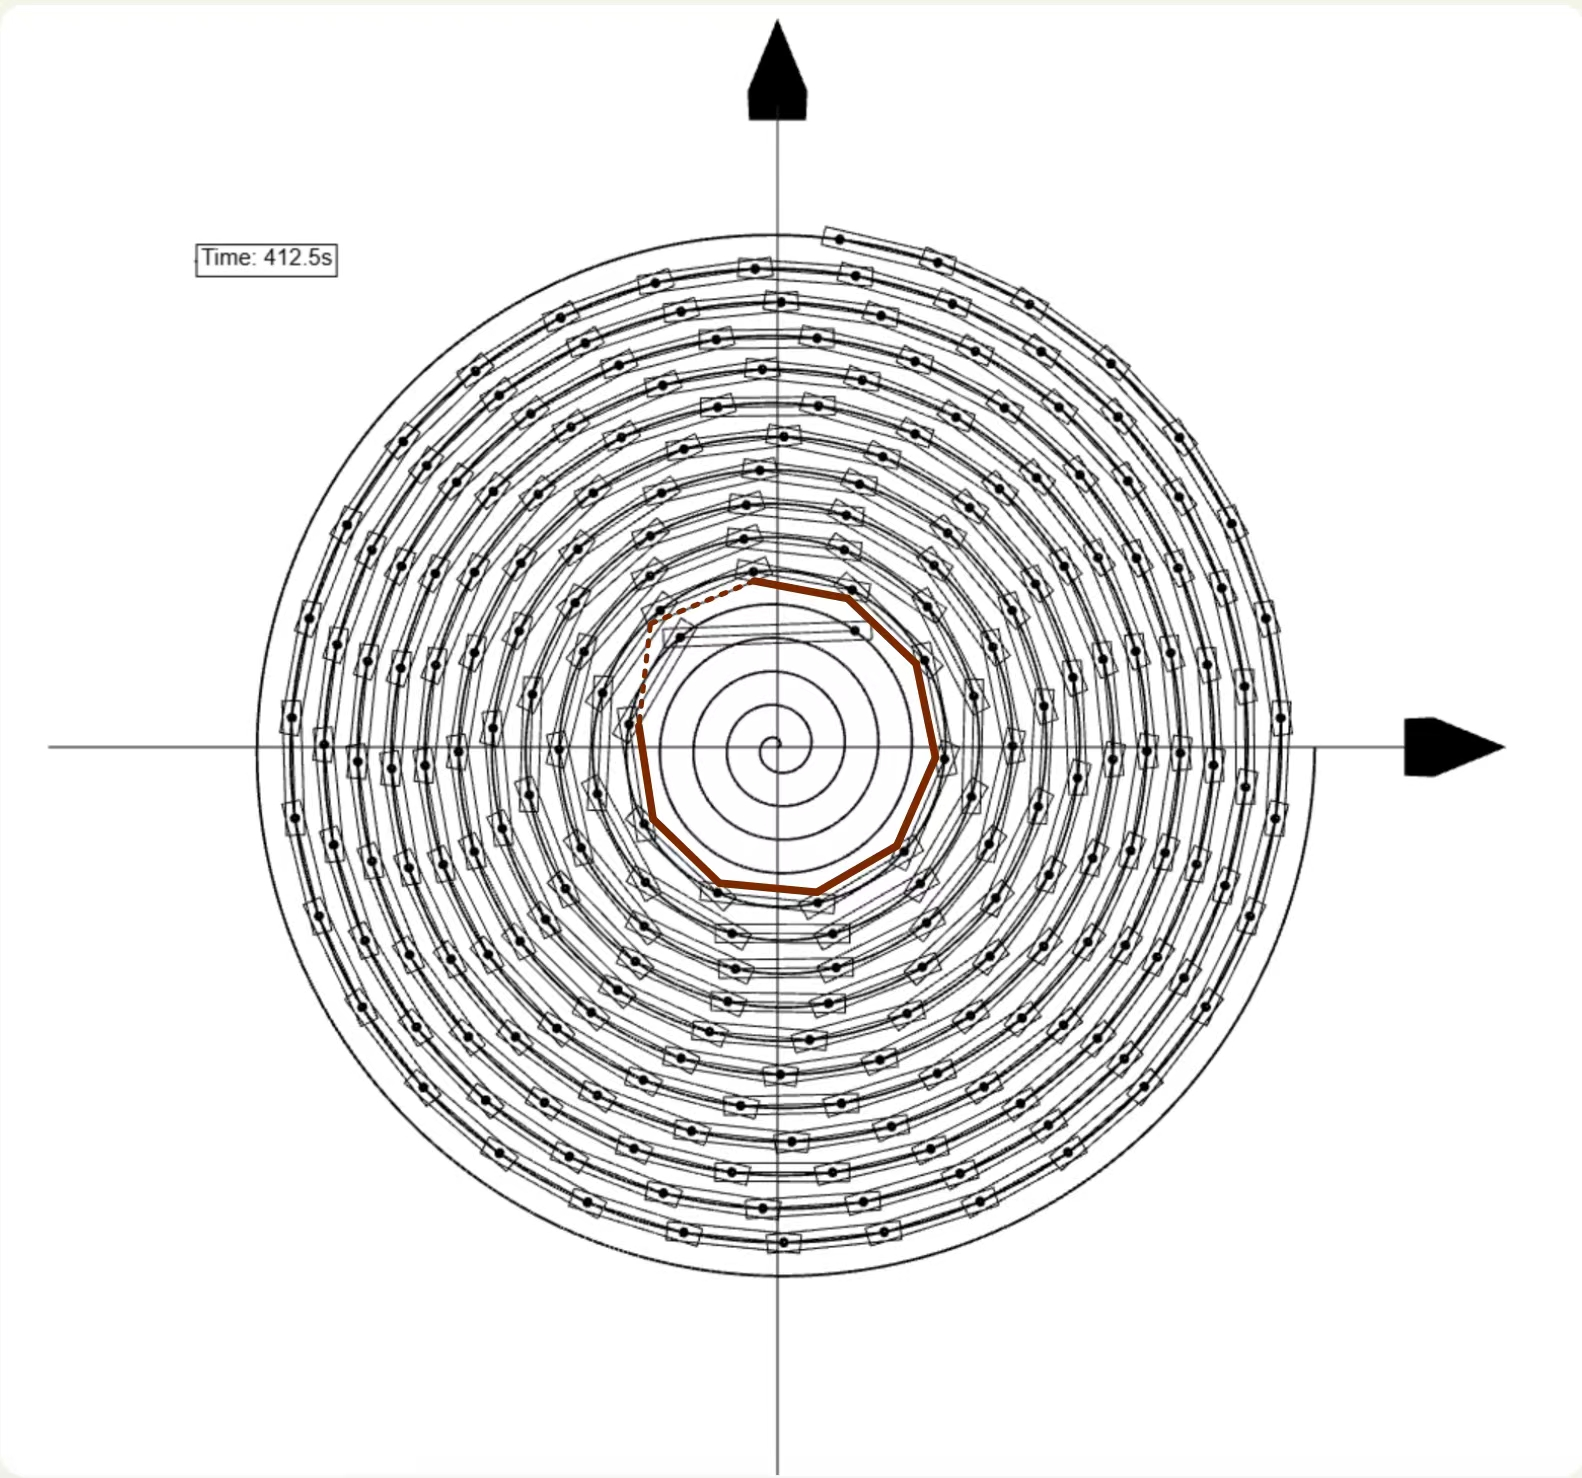
\includegraphics[width=0.4\linewidth]{image/tuji.jpg}
		    \caption{凸集构造示意图}
		    \label{fig:enter-label2}
		\end{figure}

         记所有板凳外部长边为$C_iC_{i}'$,内部长边为$B_iB_{i}'$,则板凳存在碰撞等价于存在编号i不相邻的线段$C_iC_{i}'$和$B_jB_{j}'$相交。也即
          $$ \underset{i=0}{\overset{222}{\bigcup}}\quad \underset{0\leq j \leq i - 2}{\bigcup}(B_i(t)B_{i}'(t) \bigcap C_j(t)C_{j}'(t)) = \emptyset$$
        \item {\textbf{跨立实验判定线段相交}}
        给定两条线段端点,为了快速判定其是否相交,可以建立跨立实验,如下图。当且仅当$A_0和A_1$分属直线$B_0B_1$两侧,且$B_0和B_1$分属直线$A_0A_1$两侧时,两线段相交。可以用\textbf{向量叉乘}的方向是否相反判断两点是否分属直线两侧。即线段$A_0A_1$和$B_0B_1$相交等价于$$(\overrightarrow{A_0A_1} \times \overrightarrow{A_0B_0}) \cdot (\overrightarrow{A_0A_1} \times \overrightarrow{A_0B_1}) \leq 0$$ 且 $$(\overrightarrow{B_0B_1} \times \overrightarrow{B_0A_0}) \cdot (\overrightarrow{B_0B_1} \times \overrightarrow{B_0A_1}) \leq 0$$
        
        \begin{figure}[H]
        	\centering
        	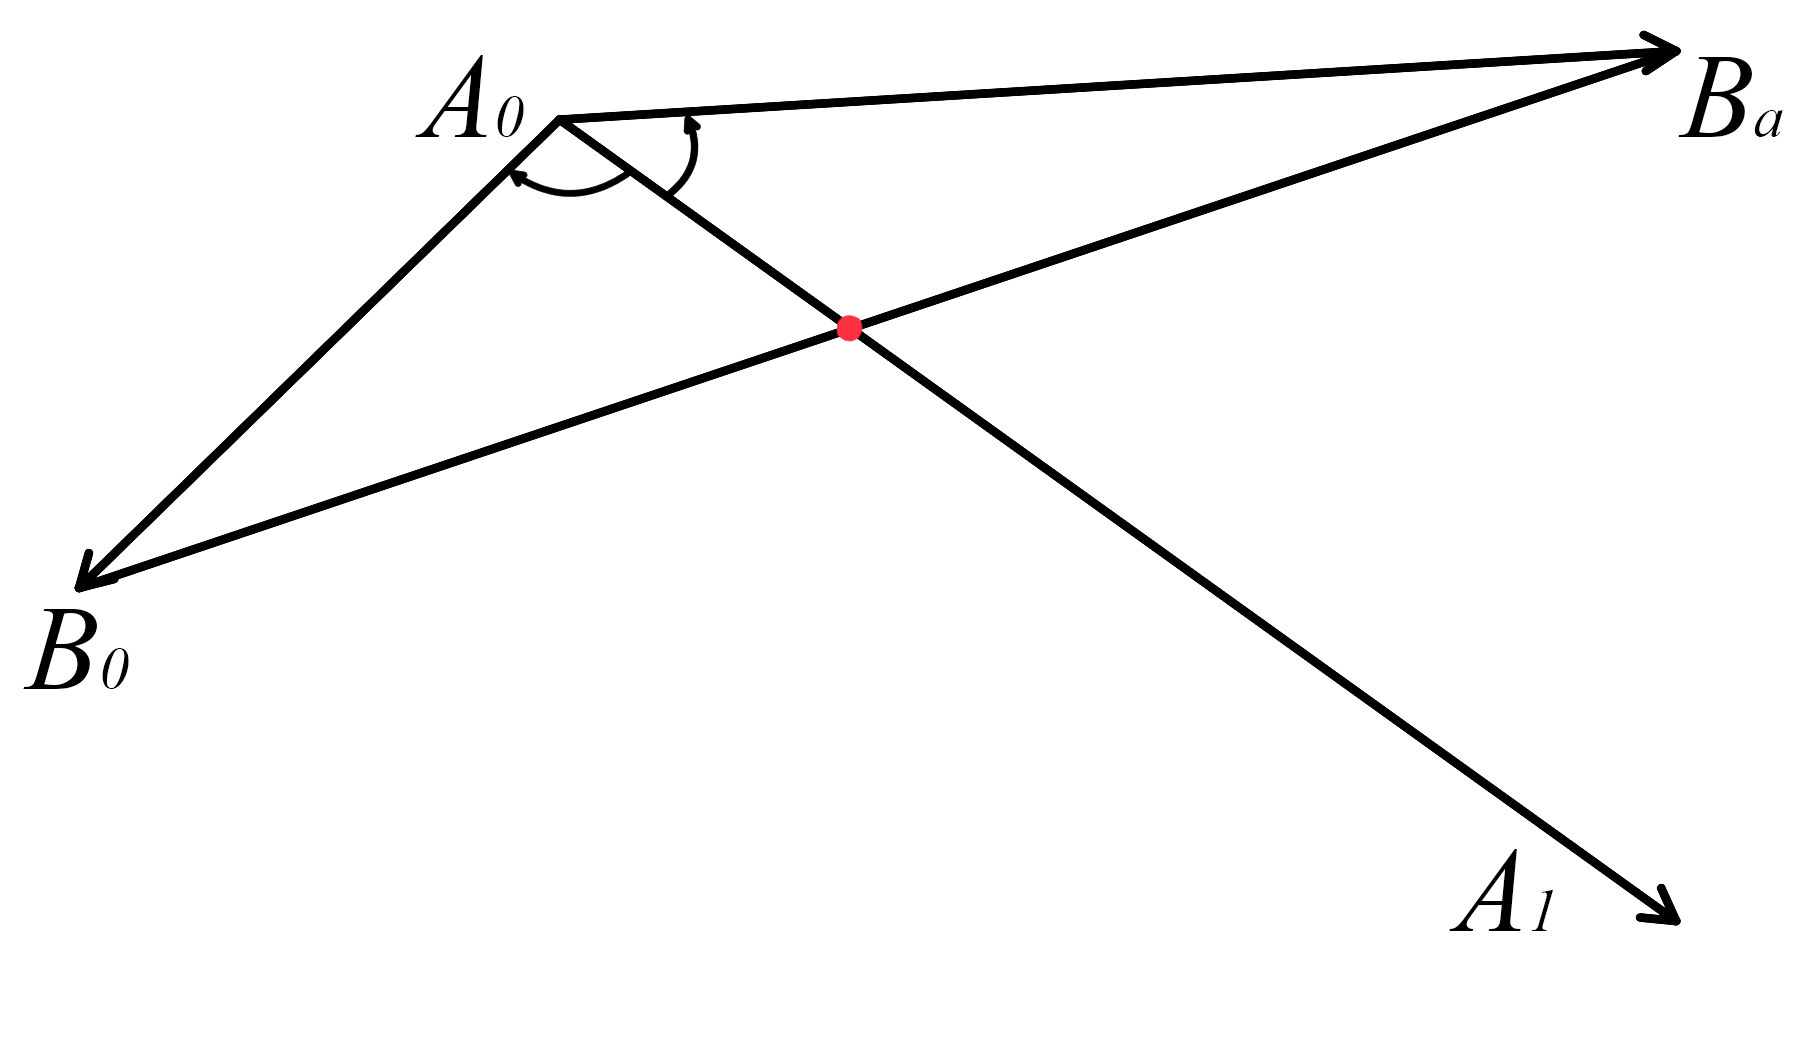
\includegraphics[width=0.5\linewidth]{image/Figure_5212.png}
        	\caption{跨立实验示意图}
        	\label{Figure_5212}
        \end{figure}
        
        \item {\textbf{最优化模型的建立}}
		以板凳龙的运动总时长t为决策变量和目标函数,结合上述线段不相交条件,最终建立了如下的单目标规划函数(其中$\phi$1-4由(6)至(9)式定义):
		\begin{equation}
			\begin{aligned}
				& \min \quad \quad t \\
				& \text { s.t. }\left\{\begin{array}{l}
                        B_i(t) = \phi_1(A_i(t), A_{i + 1}(t))\\
                        B_{i}'(t) = \phi_2(A_i(t), A_{i + 1}(t))\\
                        C_i(t) = \phi_3(A_i(t), A_{i + 1}(t))\\
                        C_{i}'(t) = \phi_4(A_i(t), A_{i + 1}(t))\\
               \underset{i=0}{\overset{222}{\bigcup}}\quad \underset{0\leq j \leq i - 2}{\bigcup}(\overline{B_i(t)B_{i}'(t)} \bigcap \overline{C_j(t)C_{j}'(t)}) = \emptyset

  \\
					% Z_k=\frac{Y_{i, y} \cdot \beta_k}{1-\alpha_k} \\
					% S_k=X_{2, y}\left(1+V_k\right)\left(1+\beta_k\right) \\
					% \beta_k \in\{1, c\} \\
					% c>1 \\

				\end{array}\right.
			\end{aligned}
		\end{equation}
    \end{itemize}
	\subsubsection{使用拟粒子群算法进行模型求解}
 通过可视化建模,初步确认板凳碰撞真值随时间增大既可能由真变假,也可能由假变真,因此通过遍历方法进行搜索需要极细粒度,计算时间过长。因此结合真值位于多个不相交区间的特点,采用粒子群算法进行求解。\textbf{其中为了求解本模型,不要求粒子位置满足约束条件,而是向最优解更新的条件中添加了约束条件,同时调整了粒子位置更新的条件。我们将调整后的算法命名为拟粒子群算法。}

\begin{figure}[H]
    \centering
    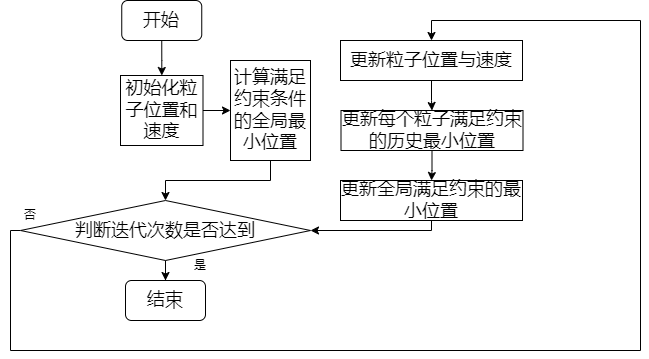
\includegraphics[width=0.8\linewidth]{image/prcess_2.png}
    \caption{拟粒子群算法流程}
    \label{fig:enter-label3}
\end{figure}

        \begin{itemize}
            \item 第一步:初始化所有粒子的位置partical[i]与速度partical\_v[i],其中位置在0-500之间随机生成,速度在0-1间随机生成(容易验证500s时保证已经有板凳相撞)。
            \item 第二步:对每个粒子所代表的时刻对应的舞龙队形态,用跨立实验判定是否相撞,如果相撞则将其与粒子的局部最小解pbest[i]比较,如更小则更新。
            \item 第三步:利用局部最小解更新全局最小解。
            \item 第四步:判断迭代次数是否达到,如达到则以全局最小解作为优化问题的解;否则更新粒子的位置,当粒子的位置超过全局最小解$\alpha$时,将其随机移动到0-$\alpha$的某一位置,以提高搜索效率。移动后回到第二步。
        \end{itemize}
该过程的代码见附录二。
        \subsubsection{使用问题一运动模型求解各把手位置坐标和速度}
        
        在问题一的求解过程中,通过二分查找算法并对各把手位置进行反复迭代计算,得到了各把手的位置信息。同时,通过将微通过分方程转换成了差分方程、微元法等方法,计算出了舞龙队各把手的速度大小。在问题二中,同样可以对把手位置进行迭代计算并二分查找,确定各把手的直角坐标位置,并使用问题一种建立的公式 (5) 利用微元法对各把手的速度大小进行求解。
        
        利用问题一中建立的运动模型,求得在恰好碰撞时刻下,舞龙队各把手的位置和速度如图所示。
        
        \begin{table}[H] %[h]表示在此处添加浮动体,默认为tbf,即页面顶部、底部和空白处添加
        	\captionsetup{skip=4pt} % 设置标题与表格的间距为4pt
        	\caption{问题二的位置结果}
        	\centering
        	\setlength{\arrayrulewidth}{0.5pt} % 设置表格线条宽度为1pt
        	\begin{tabular}{|c|c|} %c表示居中,l表示左对齐,r表示右对齐,中间添加“|”表示竖线
        		\hline
        		% \makebox[0.15\textwidth][c]{符号} & \makebox[0.6\textwidth][c]{说明}  \\
        		% \hline
        						    & 412.474213 s \\ \hline
        		龙头 x (m)           &  1.210242 \\ \hline 
        		龙头 y (m)           &  1.942574 \\ \hline
        		第 1 节龙身 x (m)    &  -1.643511 \\ \hline 
        		第 1 节龙身 y (m)    &  1.753644 \\ \hline
        		第 51 节龙身 x (m)   &  1.281550 \\ \hline 
        		第 51 节龙身 y (m)   &  4.326477 \\ \hline
        		第 101 节龙身 x (m)  &  -0.536610 \\ \hline 
        		第 101 节龙身 y (m)  &  -5.880099 \\ \hline
        		第 151 节龙身 x (m)  &  0.968478 \\ \hline 
        		第 151 节龙身 y (m)  &  -6.957525 \\ \hline
        		第 201 节龙身 x (m)  &  -7.893214 \\ \hline 
        		第 201 节龙身 y (m)  &  -1.230402 \\ \hline
        		龙尾(后) x (m)     &  0.956579 \\ \hline 
        		龙尾(后) y (m)     &  8.322691 \\ \hline
        	\end{tabular}
        	% \hline是横线,采用\makebox设置列宽
        \end{table}
        
        \begin{table}[H] %[h]表示在此处添加浮动体,默认为tbf,即页面顶部、底部和空白处添加
        	\captionsetup{skip=4pt} % 设置标题与表格的间距为4pt
        	\caption{问题二的速度结果}
        	\centering
        	\setlength{\arrayrulewidth}{0.5pt} % 设置表格线条宽度为1pt
        	\begin{tabular}{|c|c|} %c表示居中,l表示左对齐,r表示右对齐,中间添加“|”表示竖线
        		\hline
        		% \makebox[0.15\textwidth][c]{符号} & \makebox[0.6\textwidth][c]{说明}  \\
        		% \hline
        		                   &  412.474213 s \\ \hline
        		龙头 (m/s)         &  1.000000 \\ \hline
        		第 1 节龙身 (m/s)   & 0.991550 \\ \hline
        		第 51 节龙身 (m/s)  & 0.976858 \\ \hline
        		第 101 节龙身 (m/s) & 0.974551 \\ \hline
        		第 151 节龙身 (m/s) & 0.973608 \\ \hline
        		第 201 节龙身 (m/s) & 0.973091 \\ \hline
        		龙尾(后) (m/s)    & 0.972932 \\ \hline
        	\end{tabular}
        	% \hline是横线,采用\makebox设置列宽
        \end{table}
        
        \subsubsection{模型验证与螺距的灵敏度分析}
        将运动过程可视化,可验证412.474213s处板凳发生碰撞,且在此之前无板凳发生碰撞——对412.474213s之前接近碰撞,肉眼难以判断的运动系统格局进行了局部细粒度验证,证实不发生碰撞,从而验证了模型的可靠性。

        该单目标优化模型主要受到参数等距螺线螺距的影响。我们上下调整螺距,对比改变前后的板凳碰撞时间,同时对比龙头前把手与原点的最小距离。
\begin{figure}[h]
  \centering
  \begin{minipage}[t]{0.48\textwidth}
    \centering
    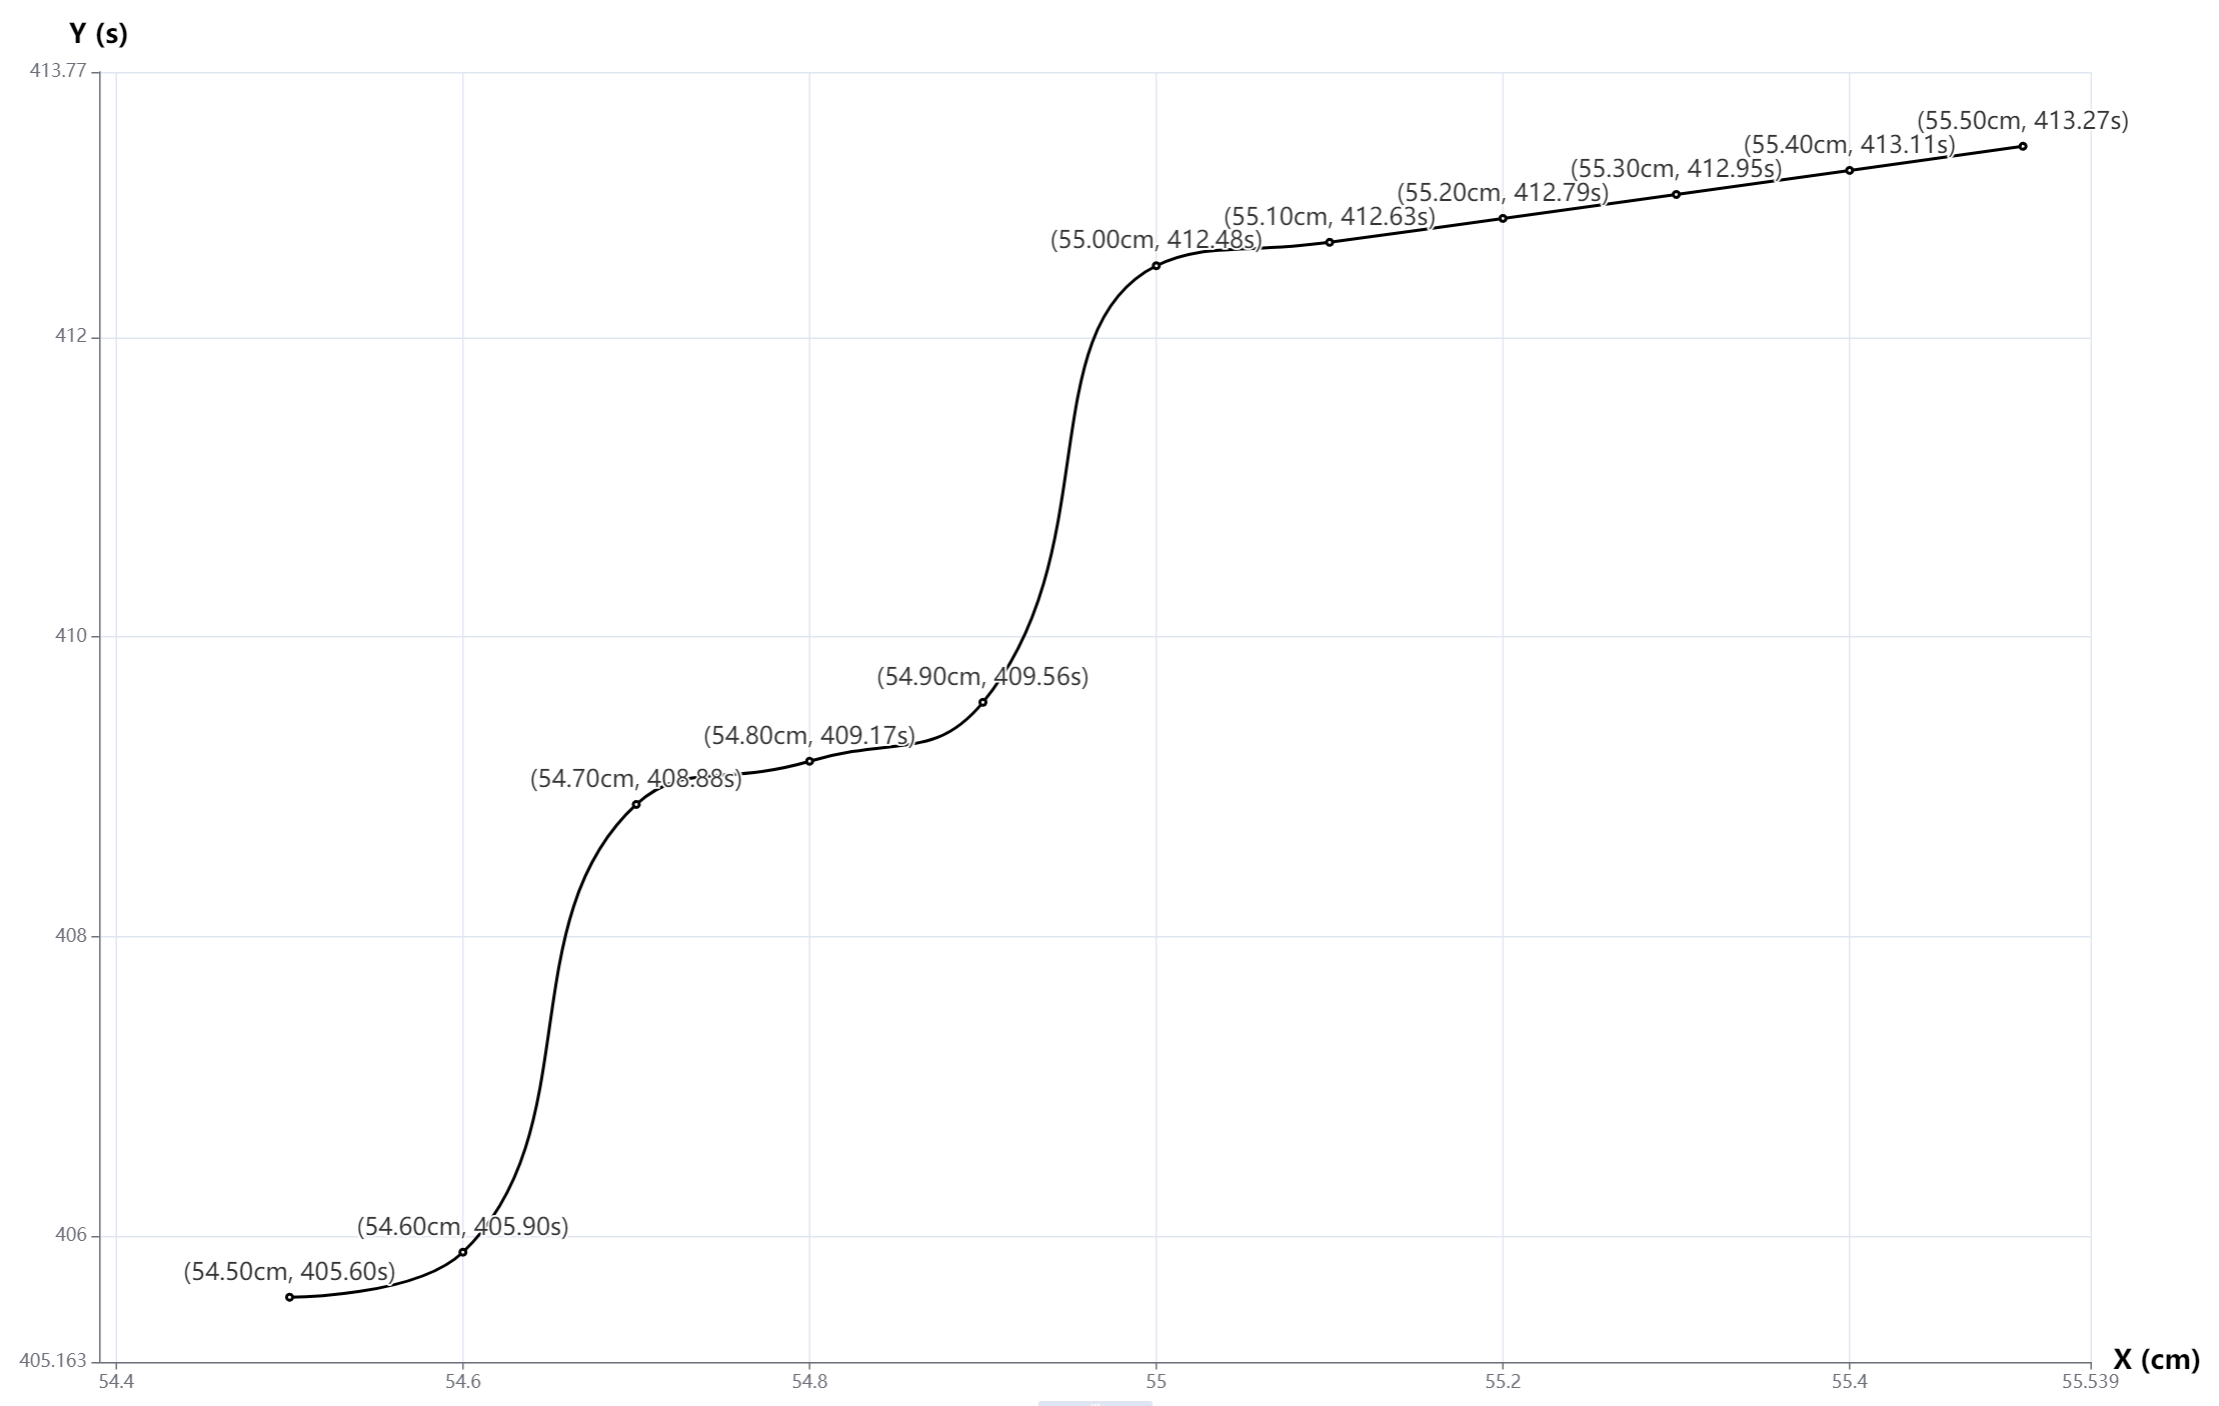
\includegraphics[width=\linewidth]{image/d_t.png}
    \caption{板凳龙碰撞的时刻关于螺距的灵敏度}
    \label{fig:left}
  \end{minipage}
  \hfill % 可选的填充,用于在两个minipage之间添加一些空间
  \begin{minipage}[t]{0.48\textwidth}
    \centering
    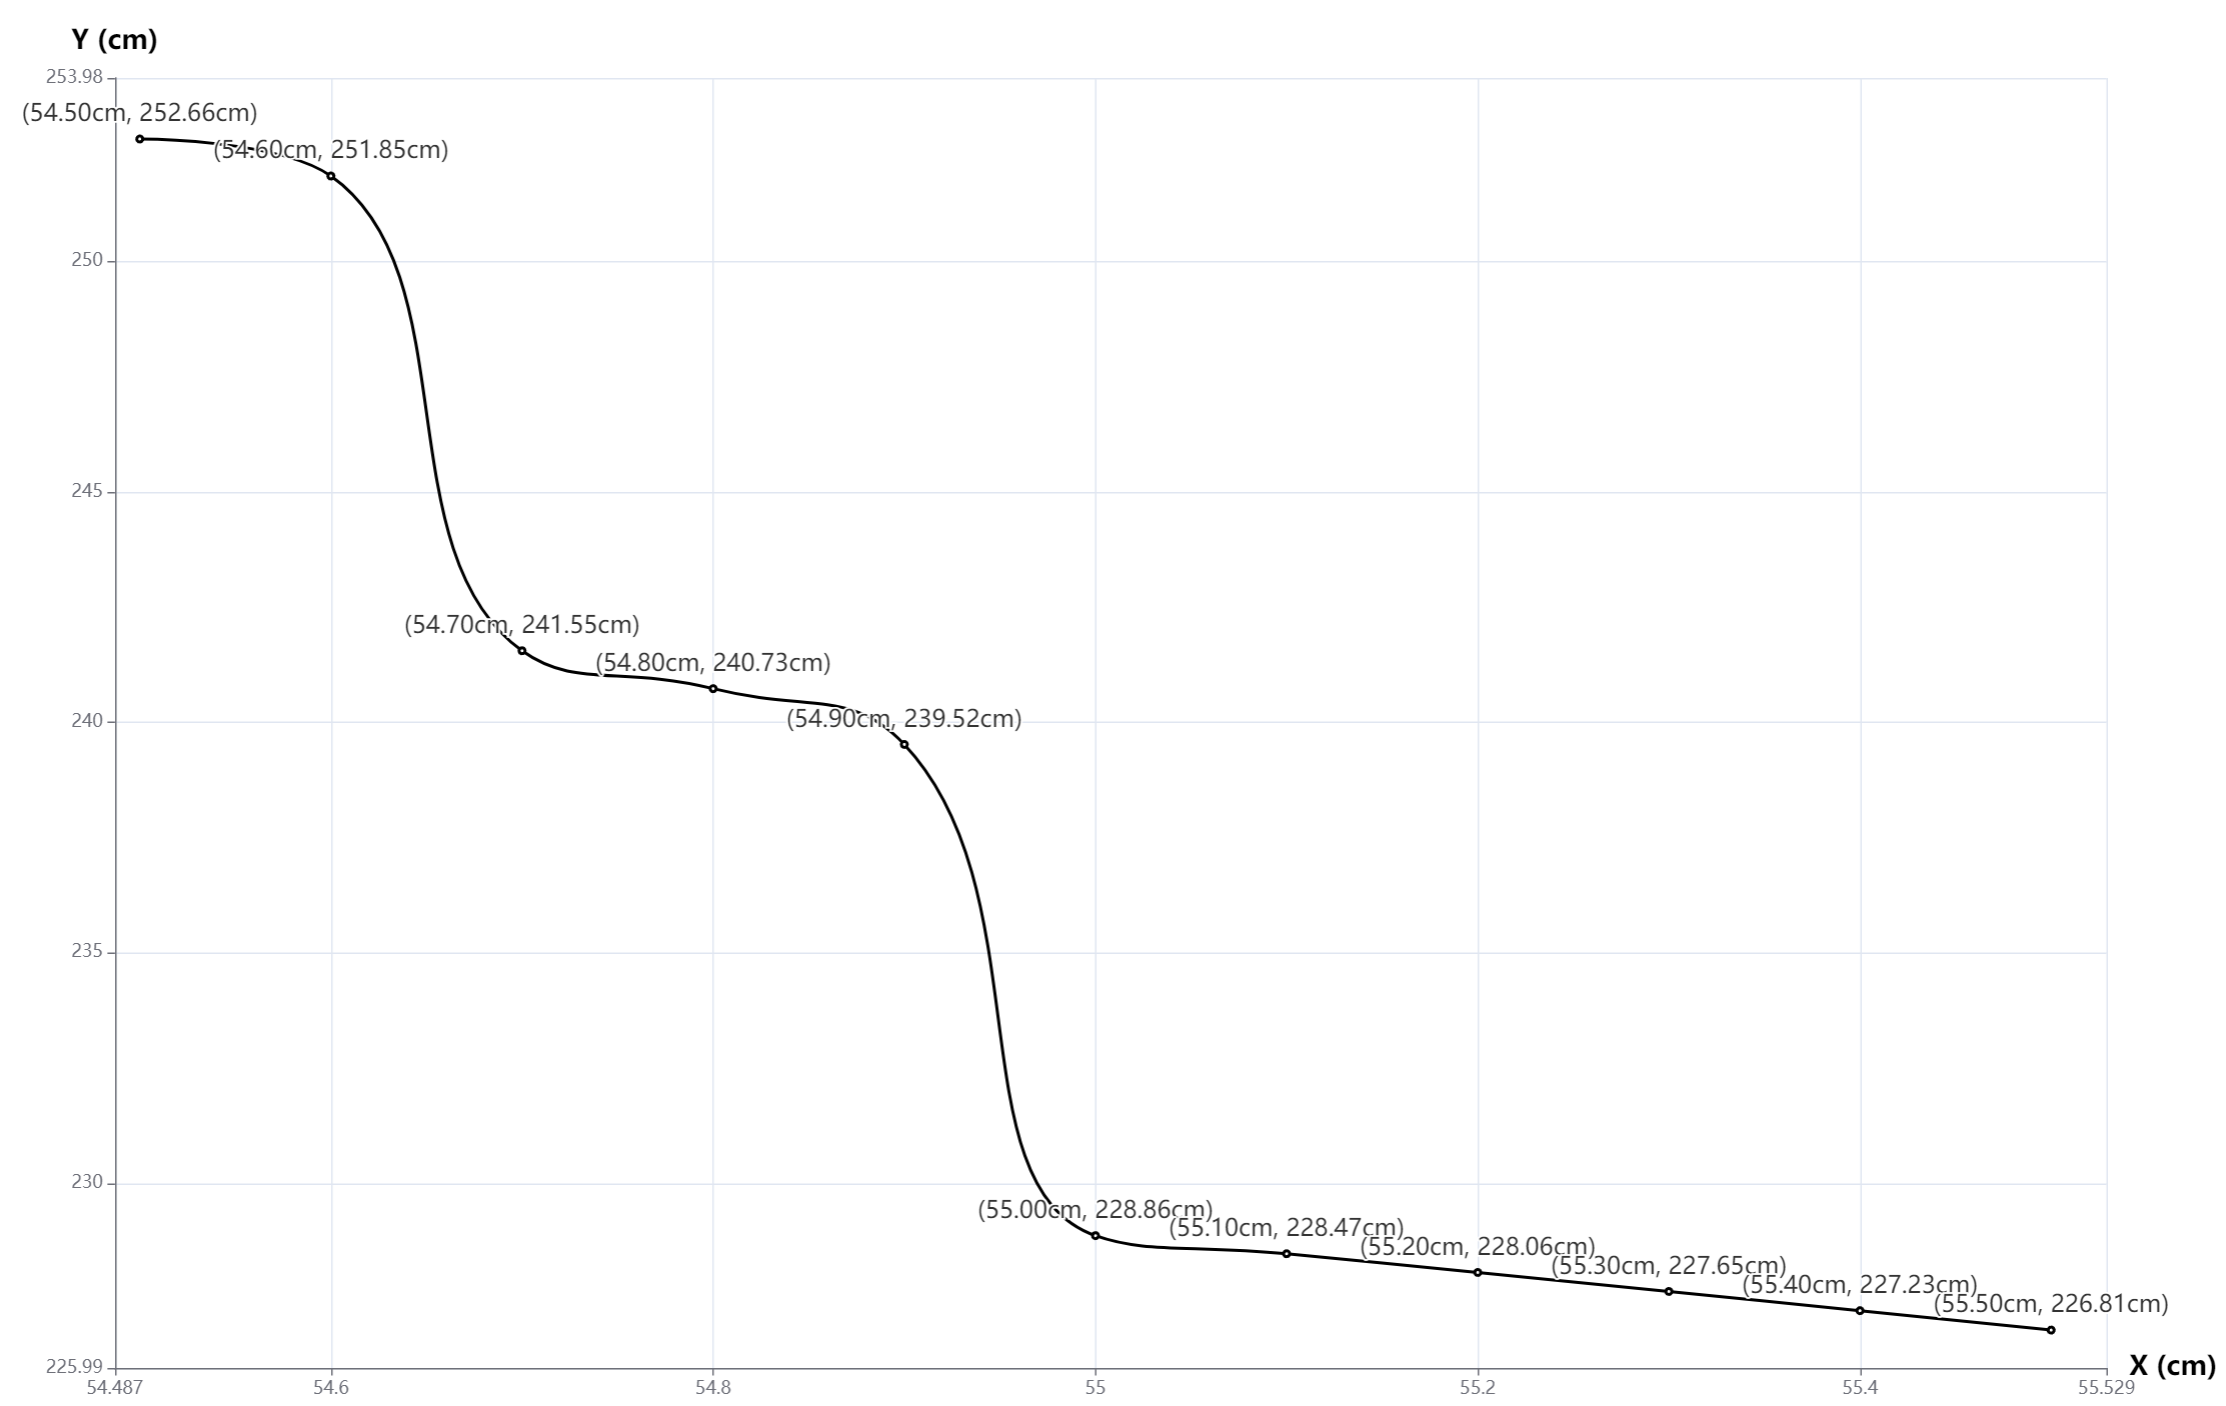
\includegraphics[width=\linewidth]{image/d_p.png}
    \caption{板凳龙碰撞时$A_0$与原点距离关于螺距的灵敏度}
    \label{fig:right}
  \end{minipage}
\end{figure}


根据实验结果,可以得到,板凳龙碰撞时刻关于螺距呈现阶梯式递增,且在螺距差为0.1cm的间隔下灵敏度表现优异。

板凳龙碰撞时刻$A_0$与原点的距离关于螺距呈现阶梯式递增,且在螺距差为0.1cm的间隔下灵敏度表现优异,为问题三的求解提供可靠支撑。
	\subsection{问题三模型的建立与求解}
 我们建立了以\textbf{等距螺线螺距}为\textbf{目标函数}的\textbf{单目标优化模型}。使用了问题二建立的模型和算法,求解出特定螺距下龙头与原点的\textbf{最小距离}。通过\textbf{可视化与回归分析}确认了螺距-龙头与原点最小距离函数的\textbf{单调性}。最后利用\textbf{二分查找}求解出满足题目要求的最小螺距为\textbf{46.269531cm}。
	\subsubsection{最优化模型的建立}
 问题三中,仍然以螺距中心为原点建立极坐标,用分别用参数方程和直角坐标表示所有研究对象的位置,在螺距变化时,以龙头前把手位于等距螺旋线第16圈的时刻作为$t = 0$的时刻。

 根据问题二的模型,添加螺距作为点的参数,我们得到某一螺距下碰撞最小时间同螺距的函数关系,即:
 		\begin{equation}
   \begin{aligned}
				& \tau(D) = \min \quad \quad t \\
				& \text { s.t. }\left\{\begin{array}{l}
                        B_i(t) = \phi_1(A_i(t, D), A_{i + 1}(t, D))\\
                        B_{i}'(t, D) = \phi_2(A_i(t, D), A_{i + 1}(t, D))\\
                        C_i(t, D) = \phi_3(A_i(t, D), A_{i + 1}(t, D))\\
                        C_{i}'(t, D) = \phi_4(A_i(t, D), A_{i + 1}(t, D))\\
               \underset{i=0}{\overset{222}{\bigcup}}\quad \underset{0\leq j \leq i - 2}{\bigcup}(\overline{B_i(t, D)B_{i}'(t, D)}\bigcap \overline{C_j(t,D)C_{j}'(t, D)} = \emptyset

  \\
					% Z_k=\frac{Y_{i, y} \cdot \beta_k}{1-\alpha_k} \\
					% S_k=X_{2, y}\left(1+V_k\right)\left(1+\beta_k\right) \\
					% \beta_k \in\{1, c\} \\
					% c>1 \\

				\end{array}\right.
    \end{aligned}
		\end{equation}


 问题三可建模为如下优化问题:求D的最小值,使得板凳龙首次碰撞的时候龙头把手与原点的距离小于4.5m。约束条件的计算分为两步,首先使用问题二的优化模型和启发式算法计算某螺距下总运行时间的最小值,其次使用问题一的参数方程模型计算运行至碰撞时龙头把手距离圆心的距离。模型的形式化描述如下:
   		\begin{equation}
   \begin{aligned}
				& \min \quad \quad D \\
				& \text { s.t. }
    \rho = \frac{D}{2 \pi} g^{-1}(\tau(D))< 4.5
    \end{aligned}
		\end{equation}
      D其中函数$g$由(4)式决定,$\tau$由(11)式决定。
        \subsubsection{模型的二分查找求解}

        用\textbf{数学证明和数据分析}可以论证$D-\rho$关系的单调性。
        若有两个不同螺距$D1 \le D2$,且$D1$螺距下在龙头把手处于$\theta$参数位置时产生碰撞,则$D2$螺距下也有龙头把手处于$\theta$参数位置时发生碰撞,且此时龙头把手距离原点的位置满足$\rho(D1, \theta) \le \rho(D2, \theta)$,这说明在更小螺距时,龙头把手能过够行进到的距离原点的最近距离。

        使用问题二的模型,简单验证可得当螺距为50cm以及超过50cm时,板凳龙会在掉头区域内部才发生碰撞;螺距为45cm时,在掉头区域外部会发生碰撞。

        对45cm至50cm螺距下板凳龙碰撞时刻龙头把手距离原点的距离进行数据分析,如下图,其中横坐标为螺距D,纵坐标为龙头前把手与原点的最小距离。可以得到$\rho$关于D的变化规律,
        \begin{itemize}
        \item $\rho$关于D递减,
        \item $\rho$关于D的变化趋势呈现阶梯式递减,即按照一定的周期先平缓递减,再迅速递减。
        \end{itemize}
\begin{figure}
    \centering
    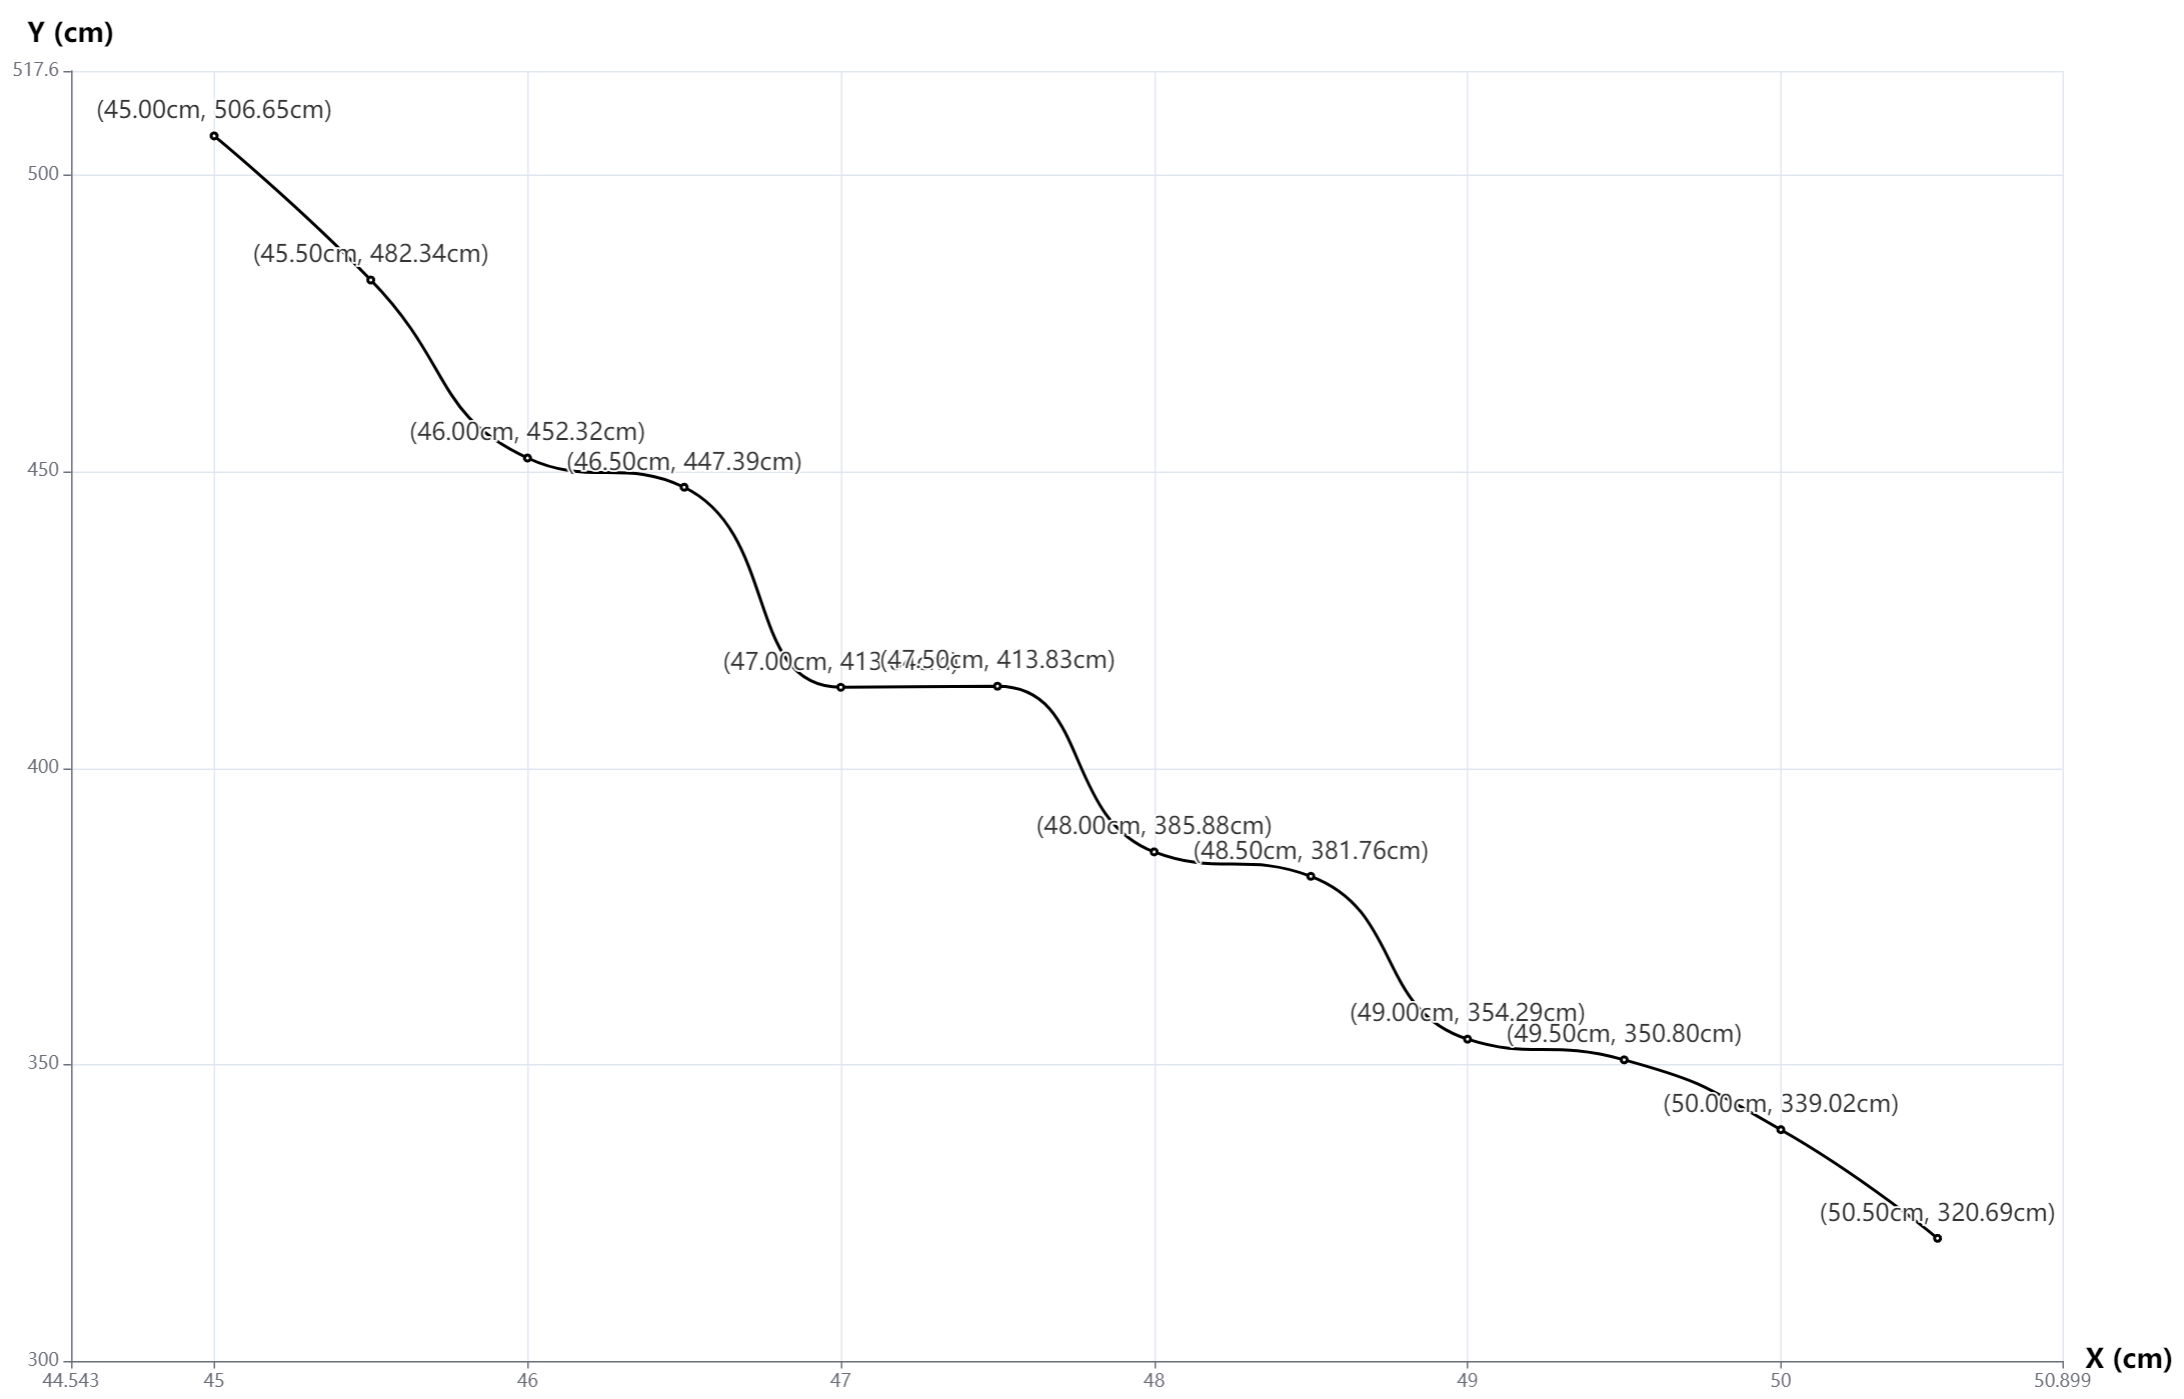
\includegraphics[width=0.5\linewidth]{image/analasis_3.png}
    \caption{45cm-55cm螺距下龙头前把手与原点最近距离}
    \label{fig:enter-label4}
\end{figure}

        因此直接采用二分查找的方式搜索$$\rho -4.5 = \frac{D}{2 \pi} g^{-1}(\tau(D)) - 4.5$$的零点,求得当D = 46.26953125cm时,$\rho$为449.94774549cm,满足题意;当D更小时$\rho$超过450cm。故满足题意的\textbf{螺距最小值为46.26953125cm}。

        下图展示了二分查找过程,横坐标为螺距,纵坐标为龙头前把手与原点的最近距离,其中虚线表示左侧的点纵坐标大于450cm,无需算出准确值。
 \begin{figure}[h]
     \centering
     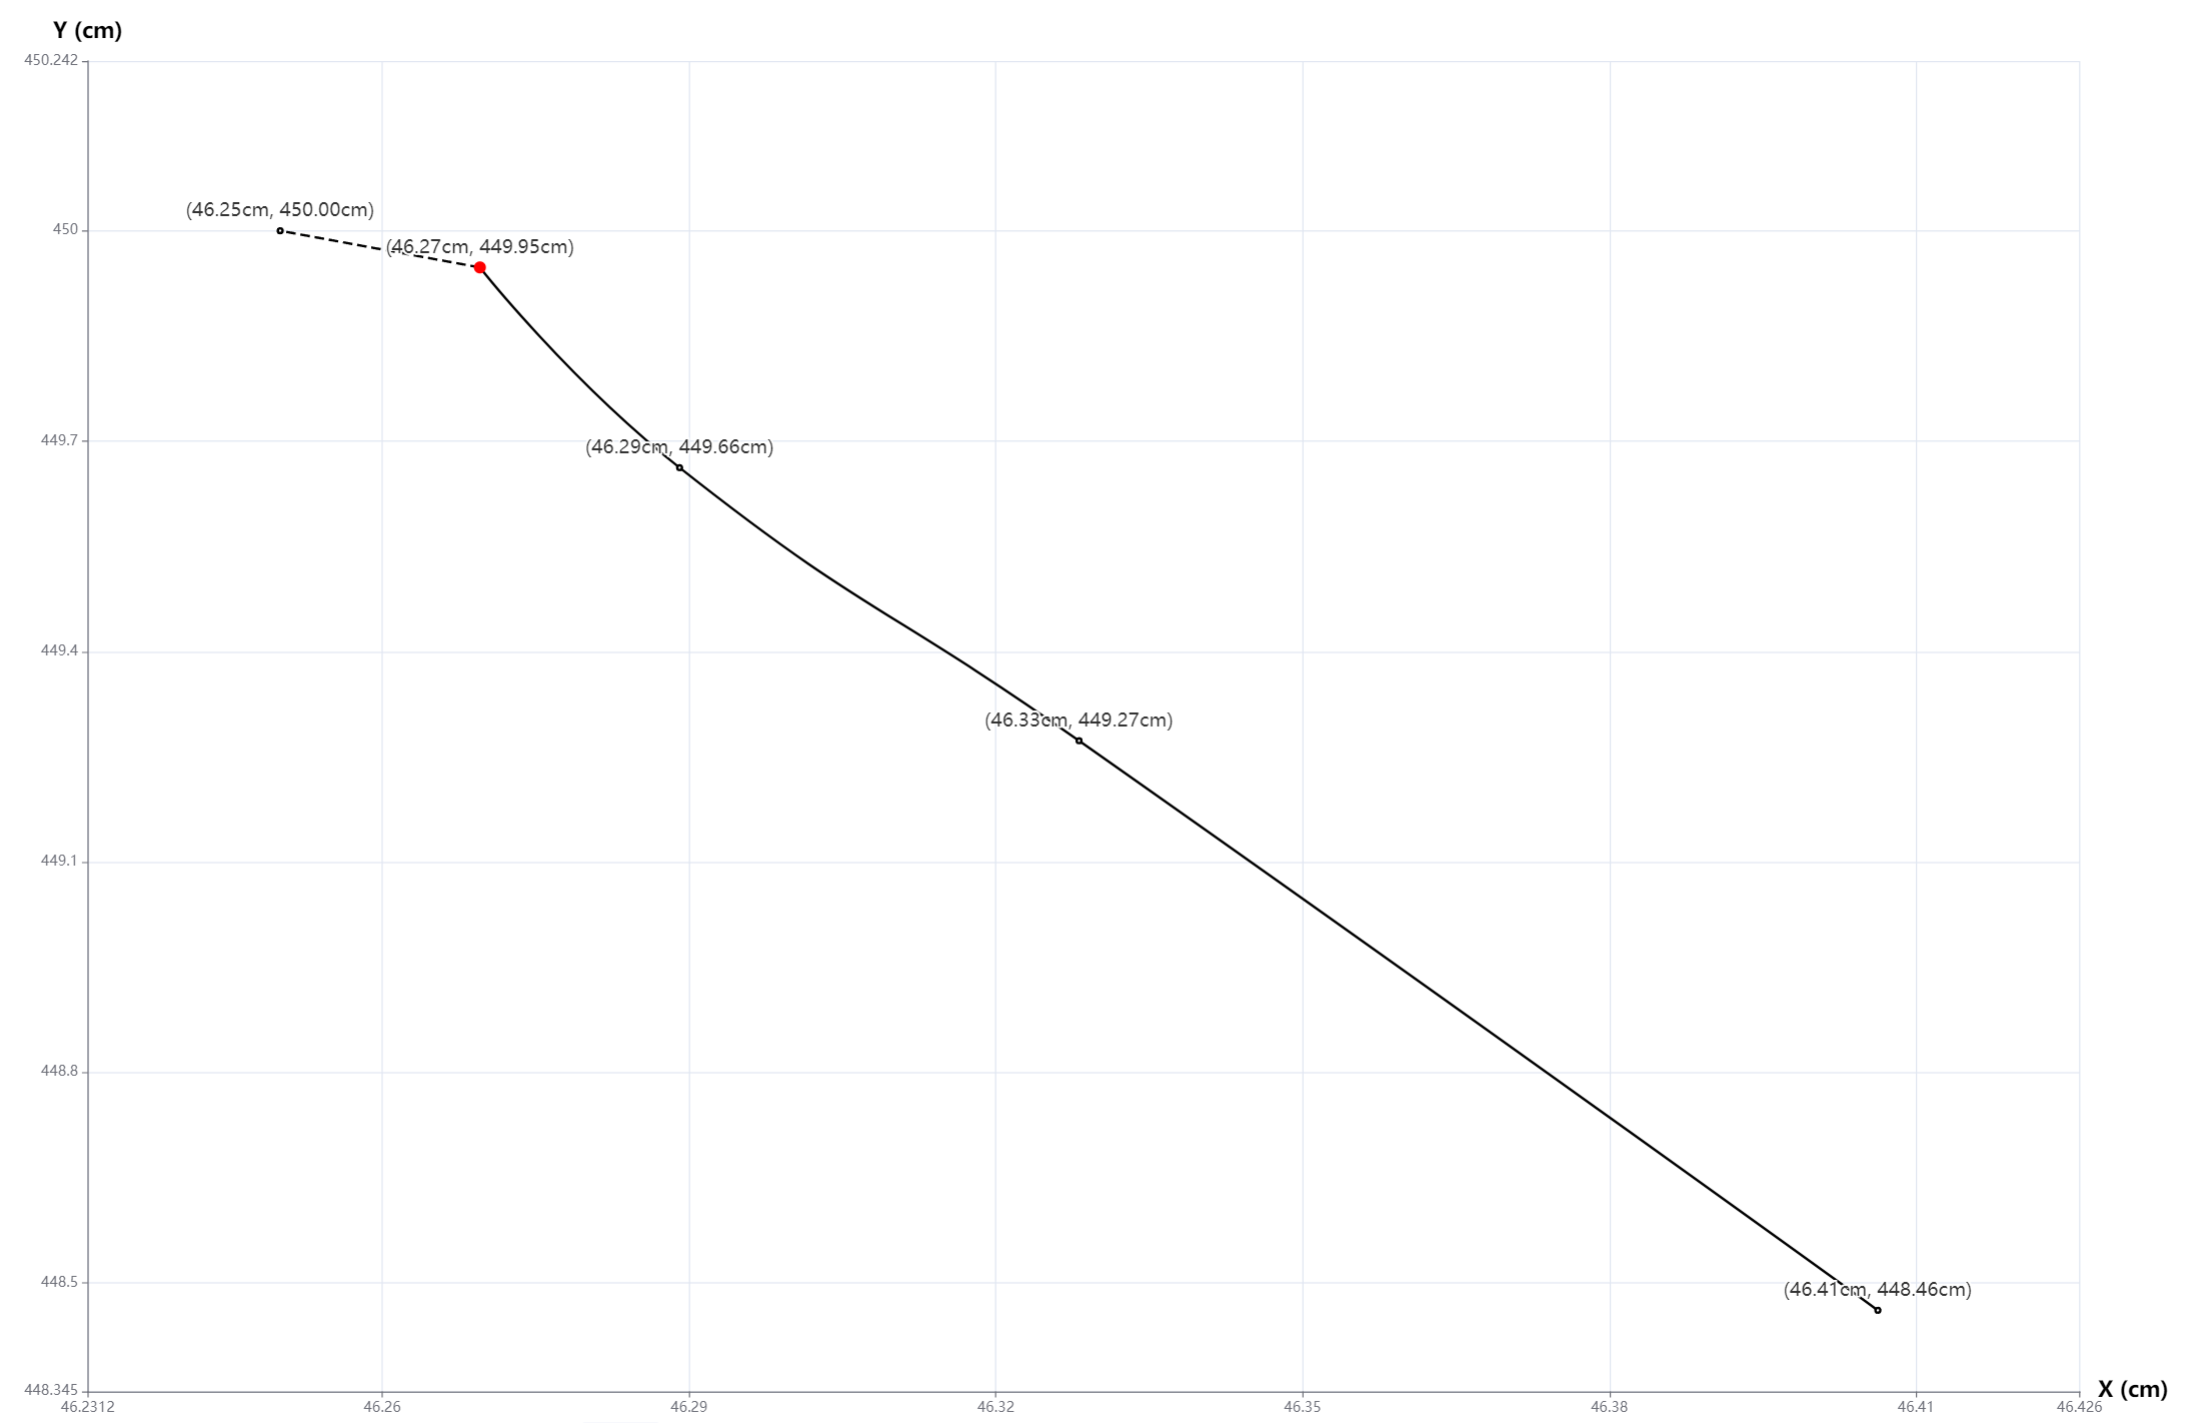
\includegraphics[width=0.5\linewidth]{image/search_3.png}
     \caption{二分查找过程示意图}
     \label{fig:enter-label5}
 \end{figure}
	\subsection{问题四模型的建立与求解}
最后,仿照问题二,将运动过程可视化,可验证龙头前把手与原点距离 449.9477cm 处板凳发生碰撞,且在此之前无板凳发生碰撞,从而验证了模型的可靠性。
		% TODO: 先说明我们是用题目中叙述的圆弧来进行建模,再叙述建模求解过程
		依据题意,建立了掉头曲线的几何模型,确定了在满足各部分相切,且前一圆弧的半径是后一圆弧半径的两倍的条件下,两圆弧的位置仅由进入和离开掉头区域的位置及方向唯一确定。因此,\textbf{在题目给定的相切约束和圆弧半径倍数的约束下,两圆弧的位置不能再优化;如果取消圆弧约束,则可以将掉头曲线直接优化为与进入位置和离开位置以尽可能小的圆弧平滑连接的一条线段}。

        在下文的所有讨论中,将严格按照全体约束条件,\textbf{确定圆弧的位置},并以该严格约束下的圆弧为掉头路径建立舞龙队\textbf{行进路线的参数方程模型},最终计算得到\textbf{舞龙队各把手的位置和速度}。% TODO

		\subsubsection{掉头曲线的几何模型及其求解}

		为了确定掉头曲线的方程使得各部分相切,\textbf{需要先求出掉头曲线的起始、结束位置的坐标和切线斜率}。
		并在此基础上\textbf{求解两圆弧的圆心位置即半径}

		由于盘出螺线和盘入螺线呈中心对称,盘入盘出螺线的极坐标方程可以表示为:

		\begin{equation}
			\rho = \frac{D}{2\pi} \theta
		\end{equation}

		\begin{equation}
			\rho = \frac{D}{2\pi} (\theta - \pi)
		\end{equation}

		而掉头区域是直径为 $R = 9$ 米的圆形区域,其圆心为原点。其极坐标方程可以表示为:

		\begin{equation}
			\rho = R
		\end{equation}

		分别联立两螺线方程和圆方程可以解得掉头区域的入口 $B$ 和出口 $B'$ 的极坐标分别为:
		$$ B(\rho, \theta) = (R, \theta_0) = (4.5, 16.631961) $$
		$$ B'(\rho, \theta) = (R, \theta_0 + \pi) = (4.5, 19.773553)$$
		换算成直角坐标即(单位:米):
		$$ (x_0, y_0) = (-2.711855, -3.591077) $$
		$$ (x_0', y_0') = (2.711855, 3.591077) $$
		确定了点 $B$ 和点 $B'$ 后,还需要确定进入掉头区域时的速度方向,用以计算相切条件。由盘入盘出螺线的中心对称性可知两点处的切线平行,斜率相同,因此只需要计算盘入曲线的切线斜率 $k$ 。

		盘入曲线的直角坐标表达式为:

		\begin{align}
			\left\{
			\begin{aligned}
				x &= \rho \cos(\theta) = \frac{D}{2\pi} \theta \cos(\theta) \\
				y &= \rho \sin(\theta) = \frac{D}{2\pi} \theta \sin(\theta)
			\end{aligned}
			\right.
		\end{align}

		在直角坐标系下取 $y$ 对 $x$ 的微分即可得到掉头曲线起始位置和结束为止的切线斜率:

		\begin{equation}
			k = \frac{dy}{dx}\Bigg|_{\theta=\theta_0} = \frac{dy}{d\theta} \frac{1}{\frac{dx}{d\theta}} \Bigg|_{\theta=\theta_0} = \frac{\sin\theta_0 + \theta_0 \cos(\theta_0)}{\cos(\theta_0) - \theta_0 \sin(\theta_0)}
		\end{equation}

		\begin{figure}[H]
			\centering
			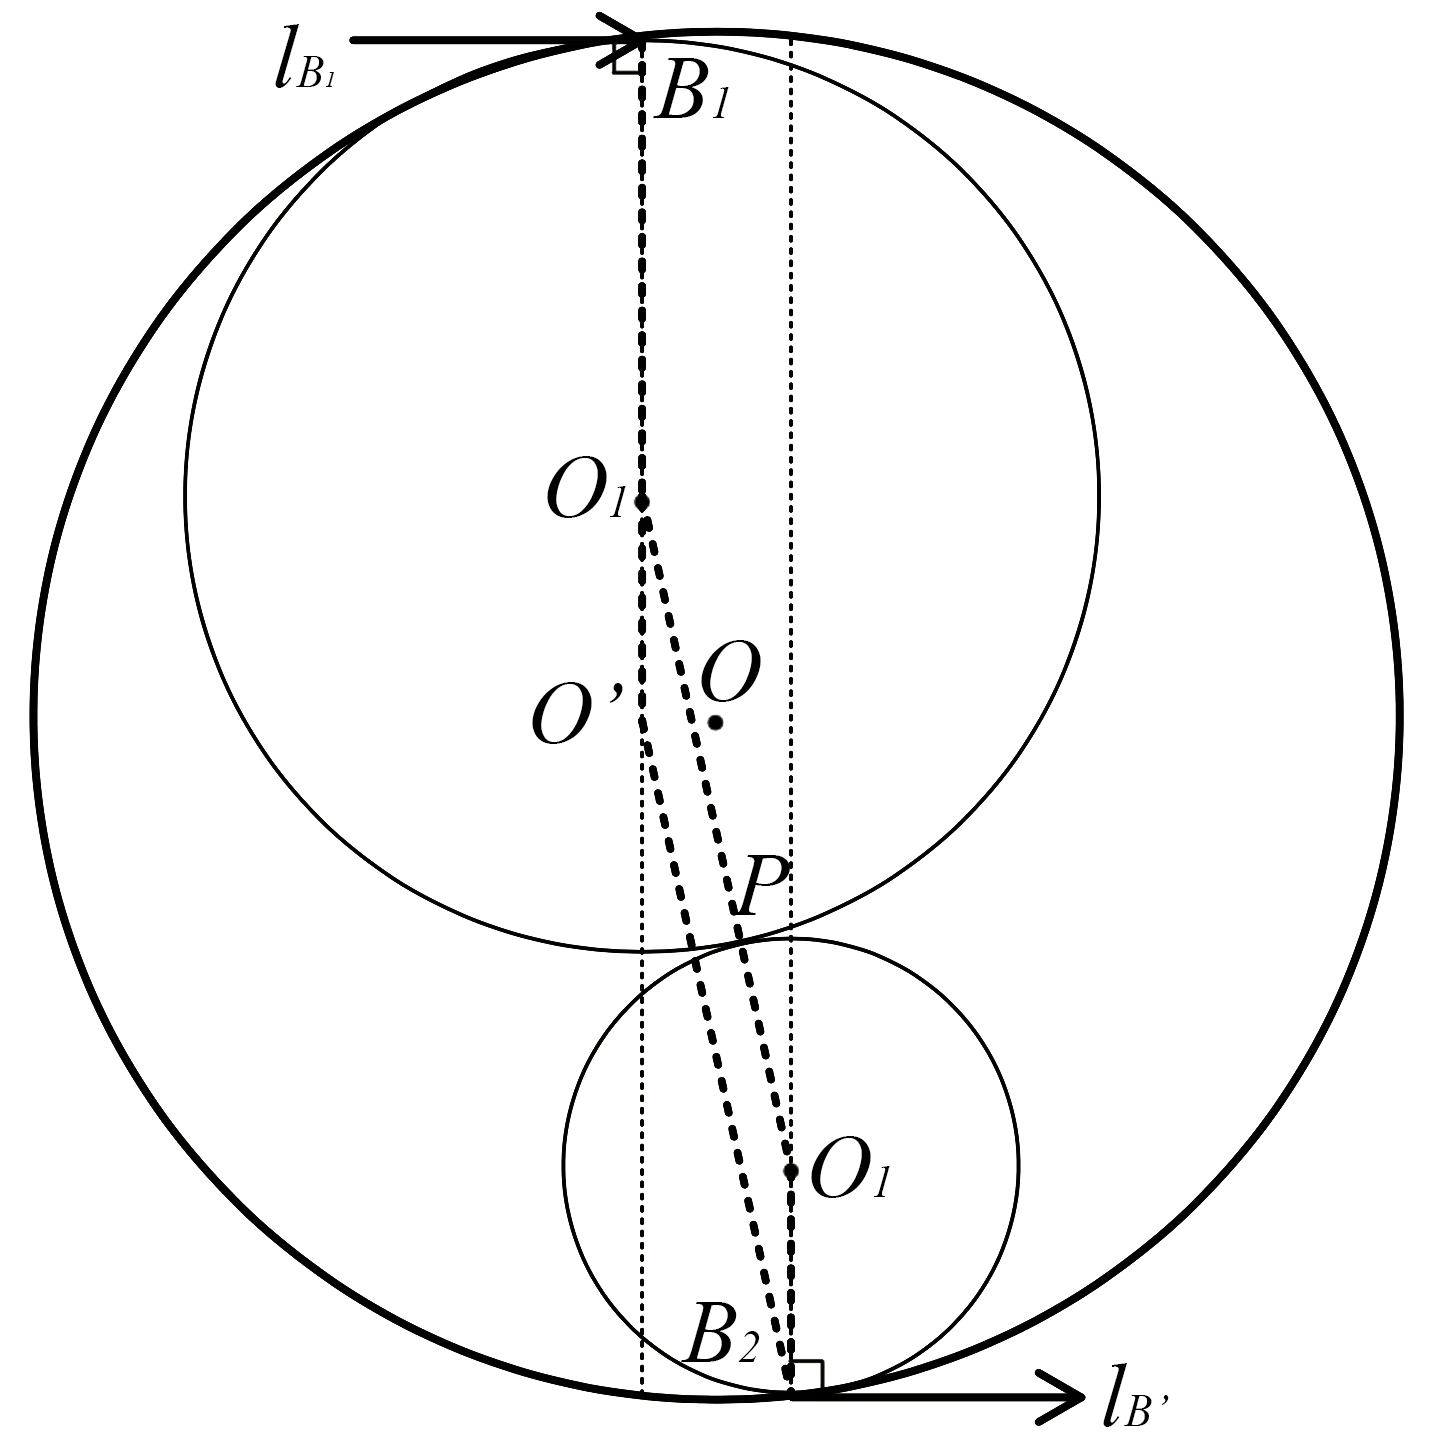
\includegraphics[width=0.5\textwidth]{image/Figure_5411.png}
			\caption{掉头曲线示意}
			\label{Figure_5411}
		\end{figure}

		如图所示 % TODO
		设前一圆弧圆心为 $O_1$ 后一圆弧圆心为 $O_2$ ,掉头曲线的起始位置和结束位置分别为点 $B$ 和点 $B'$ 。延长 $B O_1$ 至点 $O'$ 使得 $O_1O' = O_2B'$ 。设前一圆弧半径为 $r_1$ ,后一圆弧半径为 $r_2$ ,则有 $r_1 = 2r_2$ 。舞龙队的沿 $\overset{\frown}{B_1 P}$, $\overset{\frown}{PB_2}$行进。 连接 $O'B'$ 可知四边形 $O'B'O_2O1$ 为平行四边形,因此有:
		$$ O'B'= O_1O_2 = r_1 + r_2 = 3r_2 = BO_1 + O_1O' = O'B$$
		同时,由于第一段圆弧是和盘入螺线相切的,因此设 $B$ 点处的切线为 $l_B$ 则有 $O'B \perp l_B$。而 $l_B$ 的斜率为 $k$ ,因此 $O'B$ 的斜率为 $-\frac{1}{k}$ 。联立:
		\begin{align}
			\left\{
			\begin{aligned}
				O'B'=O'B \\
				\frac{x_{O'} - x_B}{y_{O'} - y_B} = -\frac{1}{k}
			\end{aligned}
			\right.
		\end{align}
		即可解得点 $O'(0.215914, -0.163050)$ 。然后,由 $\overrightarrow{OO_1} = \overrightarrow{OB_1} + 2\overrightarrow{O_1O}$ , $\overrightarrow{OO_2} = \overrightarrow{OB_2} + \overrightarrow{O'O}$ 即可解得两圆弧的圆心坐标 $O_1(x_1, y_1)$ $O_2(x_2, y_2)$

	\subsubsection{舞龙队行进路线的参数方程模型及求解}
	
		5.4.1 节得到了舞龙队行进路线中各部分路线的具体位置、参数,但是却没有将各部分曲线合并在一起,给问题四的舞龙队的速度和位置计算带来的挑战。因此,需要建立合适的参数方程来刻画整一条行进路线,即给定现实的时间 $t$ 作为参数,需要能够得到行进路线上点的参数。同时,由于龙头在任一时刻下位置就是这条曲线的参数方程,因此可以\textbf{使用龙头把手的位置与时间的函数关系作为舞龙队行进路线的参数方程}。
		
		分析可知,舞龙队的行进路线可以分为四部分:盘入阶段、前圆弧阶段、后圆弧阶段和盘出阶段。前圆弧阶段和后圆弧阶段过渡的时间节点在 $t1$ 时刻,后圆弧阶段和盘出阶段过渡的时间节点在 $t2$ 时刻。类似问题一的求解过程可以得到盘入阶段的极坐标方程为:
		
		\begin{equation}
			(\frac{1}{2}\ln(\sqrt{1 + \theta^2} - \theta) - \frac{1}{2} \theta \sqrt{\theta^2 + 1}) \frac{D}{2 \pi} - vt + C_0 = 0, \quad t \le 0
		\end{equation}
		
		在求出方程数值解后,只需要将极坐标换算成直角坐标,即可得到盘入阶段下,给定时刻 $t$ 下龙头把手的位置。
		
		对于前圆弧,只需要在直角坐标系下将圆弧转换为\textbf{圆的参数方程}即可。考虑到前圆弧的运动方向是顺时针,因此参数方程中的角速度应当为负数,即 $w = -\frac{v}{r_1}$ 
		
		\begin{equation}
			\begin{aligned}
				\left\{
					\begin{array}{l}
						x = x_1 + r_1 \cos(\theta_1 - \frac{v}{r_1}t) \\
						y = y_1 + r_1 \sin(\theta_1 - \frac{v}{r_1}t) \\
					\end{array}
				\right.
			\end{aligned}
			, \quad 0 < t \le t_1
		\end{equation}
		
		后圆弧的计算过程与前圆弧类似。考虑到后圆弧是逆时针运动,角速度应当为正,即 $w = \frac{v}{r_2} $:
		
		\begin{equation}
			\begin{aligned}
				\left\{
				\begin{array}{l}
					x = x_2 + r_2 \cos(\theta_2 - \frac{v}{r_2}t) \\
					y = y_2 + r_2 \sin(\theta_2 - \frac{v}{r_2}t) \\
				\end{array}
				\right.
			\end{aligned}
			, \quad t_1 < t \le t_2
		\end{equation}
		
		在给定初相下即可得到两圆弧的参数方程。利用解析几何可计算出前圆弧参数方程中初相 $\theta_1$ 以及后圆弧参数方程的初相 $\theta_2$ 即可确定两圆弧的参数方程。
		
		对于盘出阶段,可以类似盘入阶段进行数值计算,得到盘出阶段在极坐标下位置和时间的关系:
		
		\begin{equation}
			(- \frac{1}{2}\ln(\sqrt{1 + (\theta - \pi)^2} - (\theta - \pi)) + \frac{1}{2} (\theta - \pi) \sqrt{(\theta - \pi)^2 + 1}) \frac{D}{2 \pi} - vt + C_3 = 0, \quad t > t_2
		\end{equation}
		
		综上,对舞龙队各部分路线参数方程进行汇总即可得到总的参数方程,记录在附件%TODO
		的 t\_to\_xy\_q4() 函数中。对该函数进行绘制即可得到舞龙队的行进路线,如图%TODO
		所示。
		
		\begin{figure}[H]
			\centering
			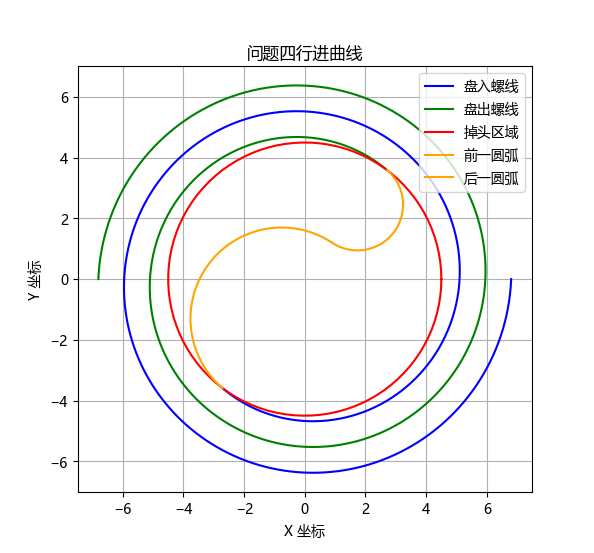
\includegraphics[width=0.7\textwidth]{image/Figure_5412.png}
			\caption{问题四舞龙队行进路线}
			\label{Figure_5412}
		\end{figure}
	
	\subsubsection{求解舞龙队的速度和位置}
	
		利用舞龙队行进路线的参数方程,以及龙头把手位置与时间的关系后,结合问题一的\textbf{二分查找算法}和\textbf{微元法}即可得到舞龙队行进的速度和位置。其中,− 100 s、− 50 s、0 s、50 s、100 s 时,龙头前把手、龙头后面第 1、
		51、101、151、201 节龙身前把手和龙尾后把手的位置和速度如表%TODO
		所示。

		\begin{table}[H] %[h]表示在此处添加浮动体,默认为tbf,即页面顶部、底部和空白处添加
			\captionsetup{skip=4pt} % 设置标题与表格的间距为4pt
			\caption{问题四的位置结果}
			\centering
			\setlength{\arrayrulewidth}{0.5pt} % 设置表格线条宽度为1pt
			\begin{tabular}{|c|c|c|c|c|c|} %c表示居中,l表示左对齐,r表示右对齐,中间添加“|”表示竖线
				\hline
				% \makebox[0.15\textwidth][c]{符号} & \makebox[0.6\textwidth][c]{说明}  \\
				% \hline
				& -100 s & -50 s & 0 s & 50 s & 100 s \\ \hline
				龙头 x (m)          & 7.778034 & 6.608301 & -2.711856 & 1.332696 & -3.157229 \\ \hline
				龙头 y (m)          & 3.717164 & 1.898865 & -3.591078 & 6.175324 & 7.548511 \\ \hline
				第 1 节龙身 x (m)   & 6.209273 & 5.366911 & -0.063534 & 3.862265 & -0.346890 \\ \hline
				第 1 节龙身 y (m)   & 6.108521 & 4.475403 & -4.670888 & 4.840828 & 8.079166 \\ \hline
				第 51 节龙身 x (m)  & -10.608038 & -3.629945 & 2.459962 & -1.671385 & 2.095033 \\ \hline
				第 51 节龙身 y (m)  & 2.831491 & -8.963800 & -7.778145 & -6.076713 & 4.033787 \\ \hline
				第 101 节龙身 x (m) & -11.922761 & 10.125787 & 3.008493 & -7.591816 & -7.288774 \\ \hline
				第 101 节龙身 y (m) & -4.802378 & -5.972247 & 10.108539 & 5.175487 & 2.063875 \\ \hline
				第 151 节龙身 x (m) & -14.351032 & 12.974784 & -7.002789 & -4.605165 & 9.462513 \\ \hline
				第 151 节龙身 y (m) & -1.980993 & -3.810357 & 10.337482 & -10.386988 & -3.540357 \\ \hline
				第 201 节龙身 x (m) & -11.952942 & 10.522509 & -6.872842 & 0.336952 & 8.524374 \\ \hline
				第 201 节龙身 y (m) & 10.566998 & -10.807425 & 12.382609 & -13.177610 & 8.606933 \\ \hline
				龙尾(后) x (m)    & -1.011059 & 0.189809 & -1.933627 & 5.859094 & -10.980157 \\ \hline
				龙尾(后) y (m)    & -16.527573 & 15.720588 & -14.713128 & 12.612894 & -6.770006 \\ \hline
			\end{tabular}
			% \hline是横线,采用\makebox设置列宽
		\end{table}
	
		\begin{table}[H] %[h]表示在此处添加浮动体,默认为tbf,即页面顶部、底部和空白处添加
			\captionsetup{skip=4pt} % 设置标题与表格的间距为4pt
			\caption{问题四的速度结果}
			\centering
			\setlength{\arrayrulewidth}{0.5pt} % 设置表格线条宽度为1pt
			\begin{tabular}{|c|c|c|c|c|c|} %c表示居中,l表示左对齐,r表示右对齐,中间添加“|”表示竖线
				\hline
				% \makebox[0.15\textwidth][c]{符号} & \makebox[0.6\textwidth][c]{说明}  \\
				% \hline
				& -100 s & -50 s & 0 s & 50 s & 100 s \\ \hline
				龙头 (m/s)          & 1.000000 & 1.000000 & 1.000000 & 1.000000 & 1.000000 \\ \hline
				第 1 节龙身 (m/s)   & 0.999904 & 0.999762 & 0.998687 & 1.000363 & 1.000124 \\ \hline
				第 51 节龙身 (m/s)  & 0.999346 & 0.998641 & 0.995134 & 0.949934 & 1.003966 \\ \hline
				第 101 节龙身 (m/s) & 0.999091 & 0.998248 & 0.994446 & 0.948479 & 1.096262 \\ \hline
				第 151 节龙身 (m/s) & 0.998944 & 0.998047 & 0.994154 & 0.948035 & 1.095306 \\ \hline
				第 201 节龙身 (m/s) & 0.998849 & 0.997925 & 0.993992 & 0.947820 & 1.094933 \\ \hline
				龙尾(后) (m/s)    & 0.998817 & 0.997885 & 0.993942 & 0.947757 & 1.094833 \\ \hline
			\end{tabular}
			% \hline是横线,采用\makebox设置列宽
		\end{table}
	
	\subsection{问题五模型的建立与求解}
	
	\subsubsection{确定把手速度分布规律}
	
		为了确定给定龙头把手下各把手的最大速度分布,需要先考察所有把手中速度的最大值关于时间的分布规律。
		
		通过对问题一、问题二的速度分析可以看出:在盘入螺线中,靠近龙头的把手的速度比靠近龙尾的速度更快。具体来说,在曲线\textbf{同方向盘绕}、曲率半径大于板凳前后把手中心间距,且\textbf{曲率单调变化}时,\textbf{位于较大曲率位置把手的速度比位于较小曲率位置把手的速度大}。下面给出证明。
		
		如图%TODO
		$A_i$,$A_{i+1}$分别为某一板凳的前把手和后把手,靠 $A_i$ 侧的曲线曲率逐渐增大。板凳 $A_iA_{i+1}$ 可视为一运动线段。在盘入阶段,$\overline{A_iA_{i+1}}$ 运动方向如图所示,设 $\overline{A_iA_{i+1}}$ 在时间 $\Delta t$ 内运动到了 $\overline{A_i'A_{i+1}'}$ 位置。由于曲率随运动而增大,对于弧 $\overset{\frown}{A_i'A_{i+1}'}$ 的曲率岛屿弧 $ \overset{\frown}{A_iA_{i+1}} $的,进而两弧满足 $|\overset{\frown}{A_i'A_{i+1}'}| > |\overset{\frown}{A_iA_{i+1}}| $关系。 因此,$A_i$ 点和 $A{i+1}$ 点的平均运动速度即满足关系:
		
		\begin{equation}
			\overline{v_{i}} = \dfrac{\overset{\frown}{A_iA_i'}}{\Delta t} \ge
			\frac{\overset{\frown}{A_{i+1}A_{i+1}'}}{\Delta t} = \overline{v_{i+1}}
		\end{equation}
		
		命题得证。
		
		据此,可以得到以下结论:
		\begin{enumerate}
			\item 经过的盘入螺线的曲率随时间推移而逐渐增大,因此在\textbf{盘入阶段龙身各把手的速度均小于龙头速度}。但是由于\textbf{等距螺线的曲率变化较小},导致\textbf{龙头龙尾的速度大小差距较小}。
			
			\item 同理,经过的盘出螺线的曲率随时间推移而逐渐减小,\textbf{在盘出阶段,龙身各把手的速度均大于龙头速度}。类似地,龙头龙尾的速度差异应当也十分小。
			
			\item 注意到在龙尾尚未进入掉头区域、龙头已经离开掉头区域的时间范围内,对于掉头区域内的板凳而言,每隔一定时间间隔,\textbf{第 i 个板凳的位置就会被下一板凳(即第 i+1 个板凳)取代,且取代后掉头区域内的速度关联关系保持不变}。因此,在这一段时间内,掉头区域内的最大速度整体取决于盘出曲线外把手的速度(随时间缓慢递增),掉头区域内把手的最大速度\textbf{整体随时间推移而缓慢递增}。此外,在第 i 个板凳的位置被下一板凳取代的过程中,\textbf{最大速度会随时间变化而发生波动},并在取代完成后重复上一波动过程。
			
			\item 考虑到龙首前后把手中心的距离比龙身和龙尾的中心距更大,且\textbf{掉头曲线的曲率较大},\textbf{曲率对板凳前后两把手关联速度}的影响会比在盘出螺线和盘出螺线内\textbf{更大}。因此,从\textbf{龙头前把手进入掉头区域,到龙头后把手离开掉头区域的过程内,靠近龙头的把手的速度会有较为明显的提升。}
		\end{enumerate}
		
		对舞龙队从 -40s 到 400 s的各把手最大速度进行分析,结果如图 %TODO
		和图%TODO
		所示,其中纵轴表示所有把手速度中的最大值,即:
		$$v_{max} = \max\{{v_i}\}$$.
		
		可以发现物理模拟结果与猜想基本一致。根据数学计算、逻辑推理和实验验证,我们\textbf{将最大速度确定在 $t \in [9s,18s]$ 的范围内},并对最大速度在此范围内进行\textbf{求解}和\textbf{验证}。
		
		\begin{figure}[H]
			\centering
			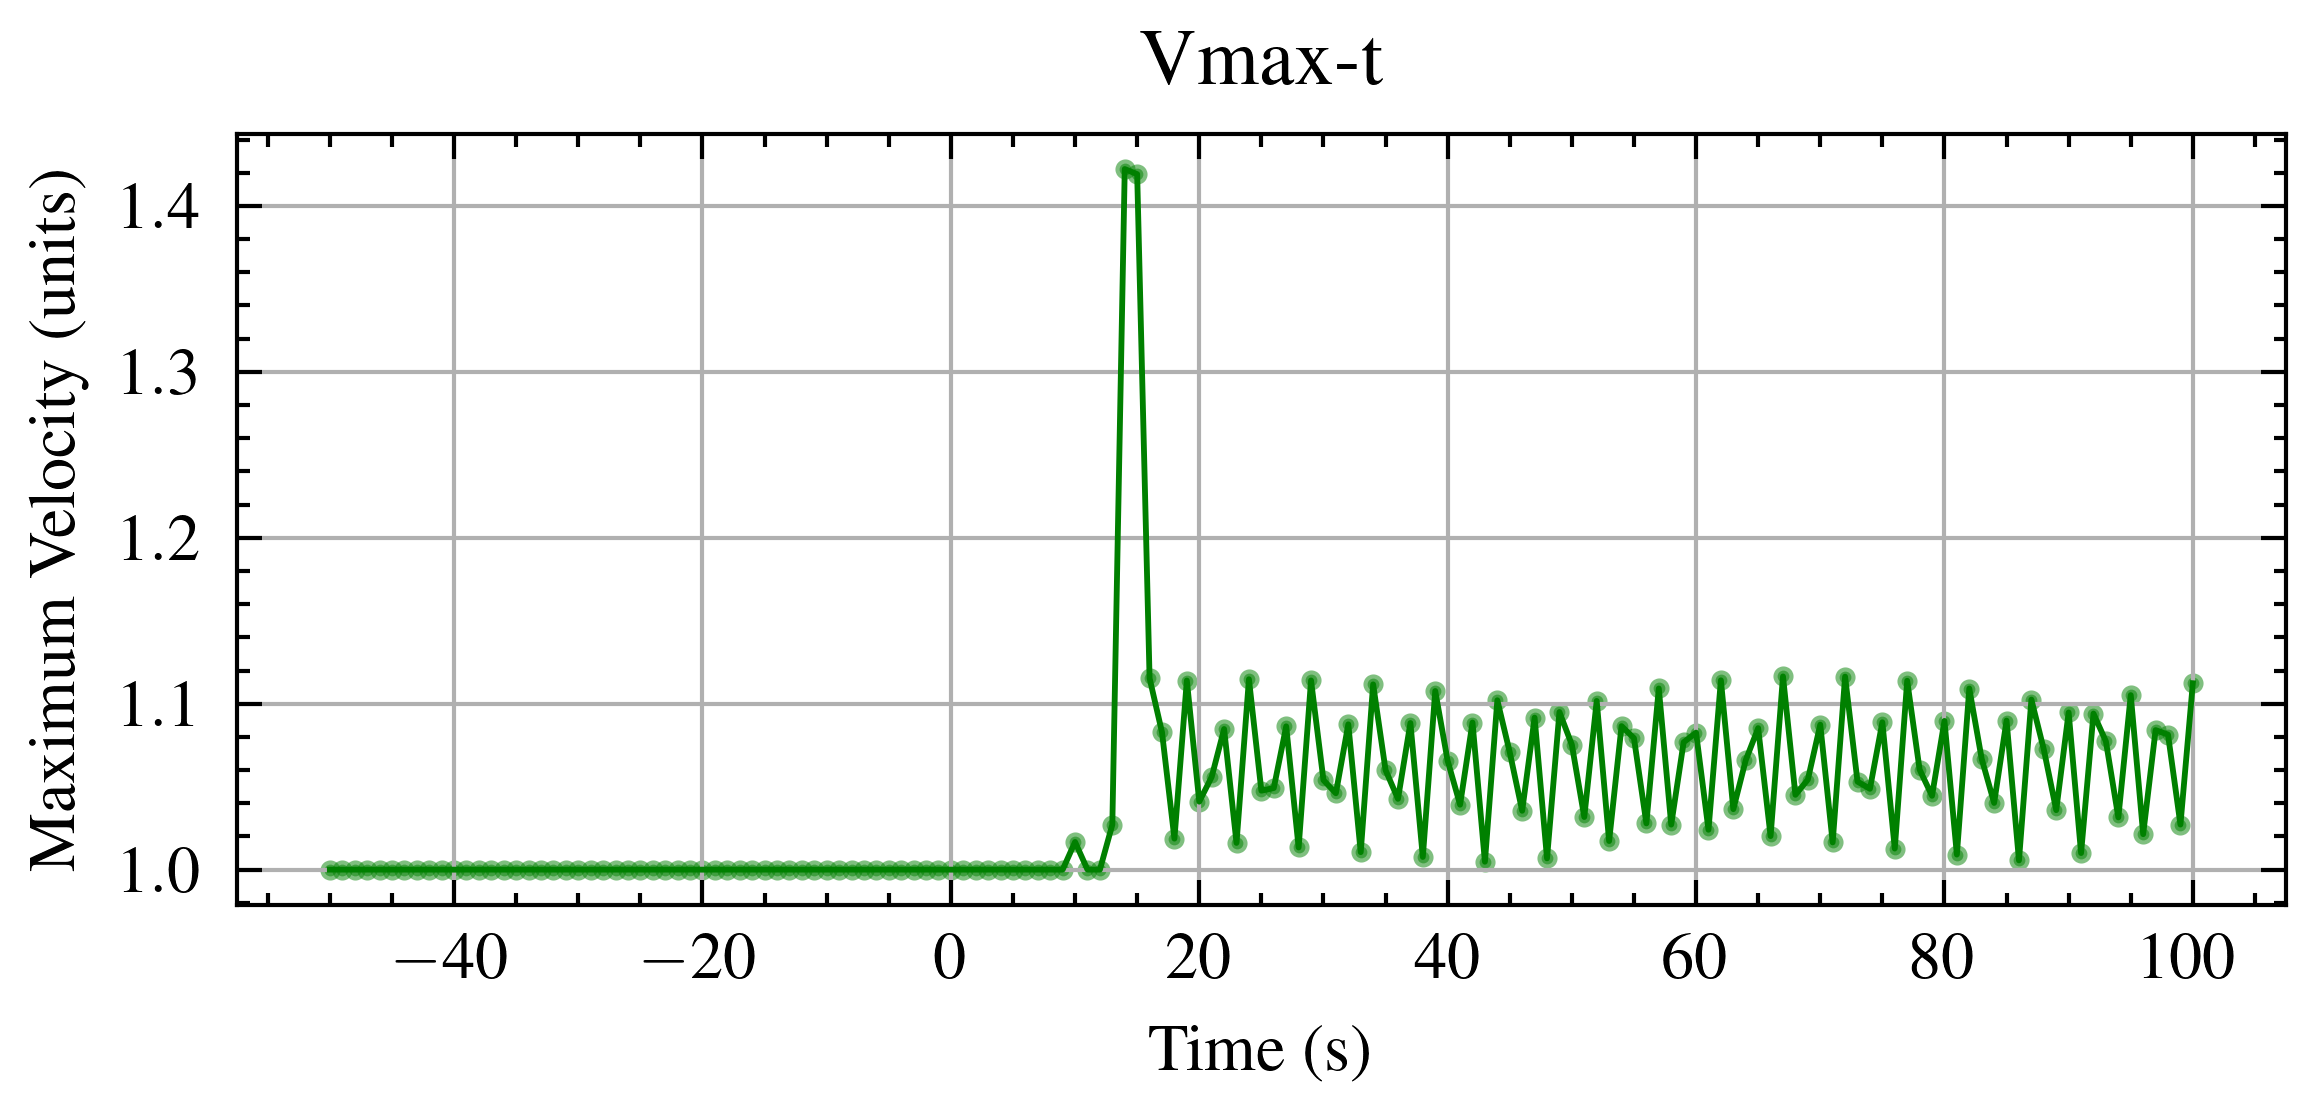
\includegraphics[width=0.6\textwidth]{image/Figure_5511.png}
			\caption{问题五最大速度关于时间的函数}
			\label{Figure_5511}
		\end{figure}
	
		\begin{figure}[H]
			\centering
			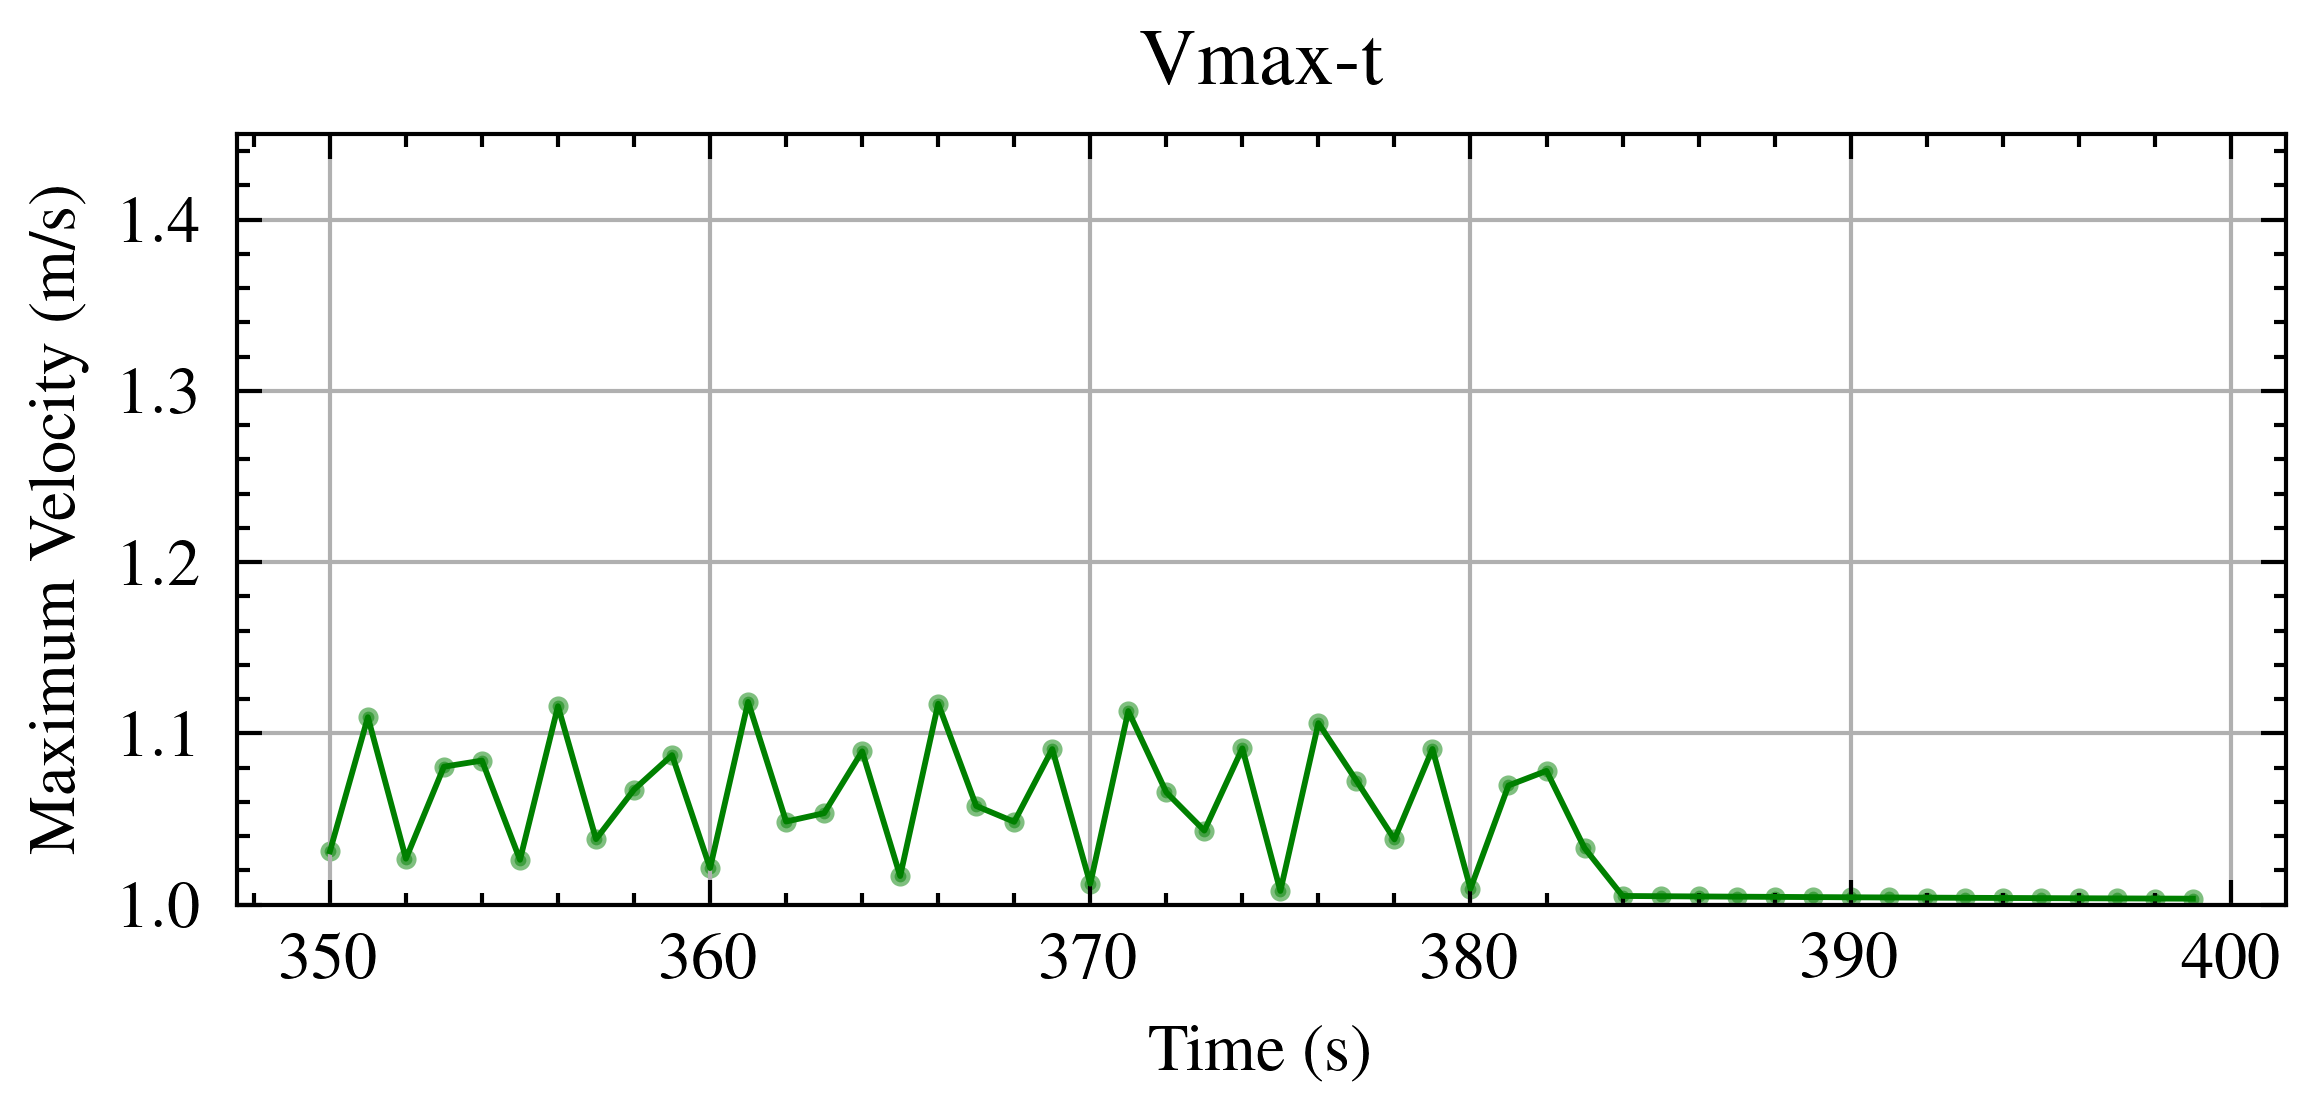
\includegraphics[width=0.6\textwidth]{image/Figure_5512.png}
			\caption{问题五最大速度关于时间的函数}
			\label{Figure_5512}
		\end{figure}
		
	\subsubsection{利用模拟退火算法求解速度最大值}
	
		确定了最大速度的区间范围后,原问题转换成了最优解的求解问题。\textbf{先对求解区域内的目标函数进行考察}。取 0.01s 作为步长绘制舞龙队最大把手速度关于时间的函数,结果如图%TODO
		所示
		
		\begin{figure}[H]
			\centering
			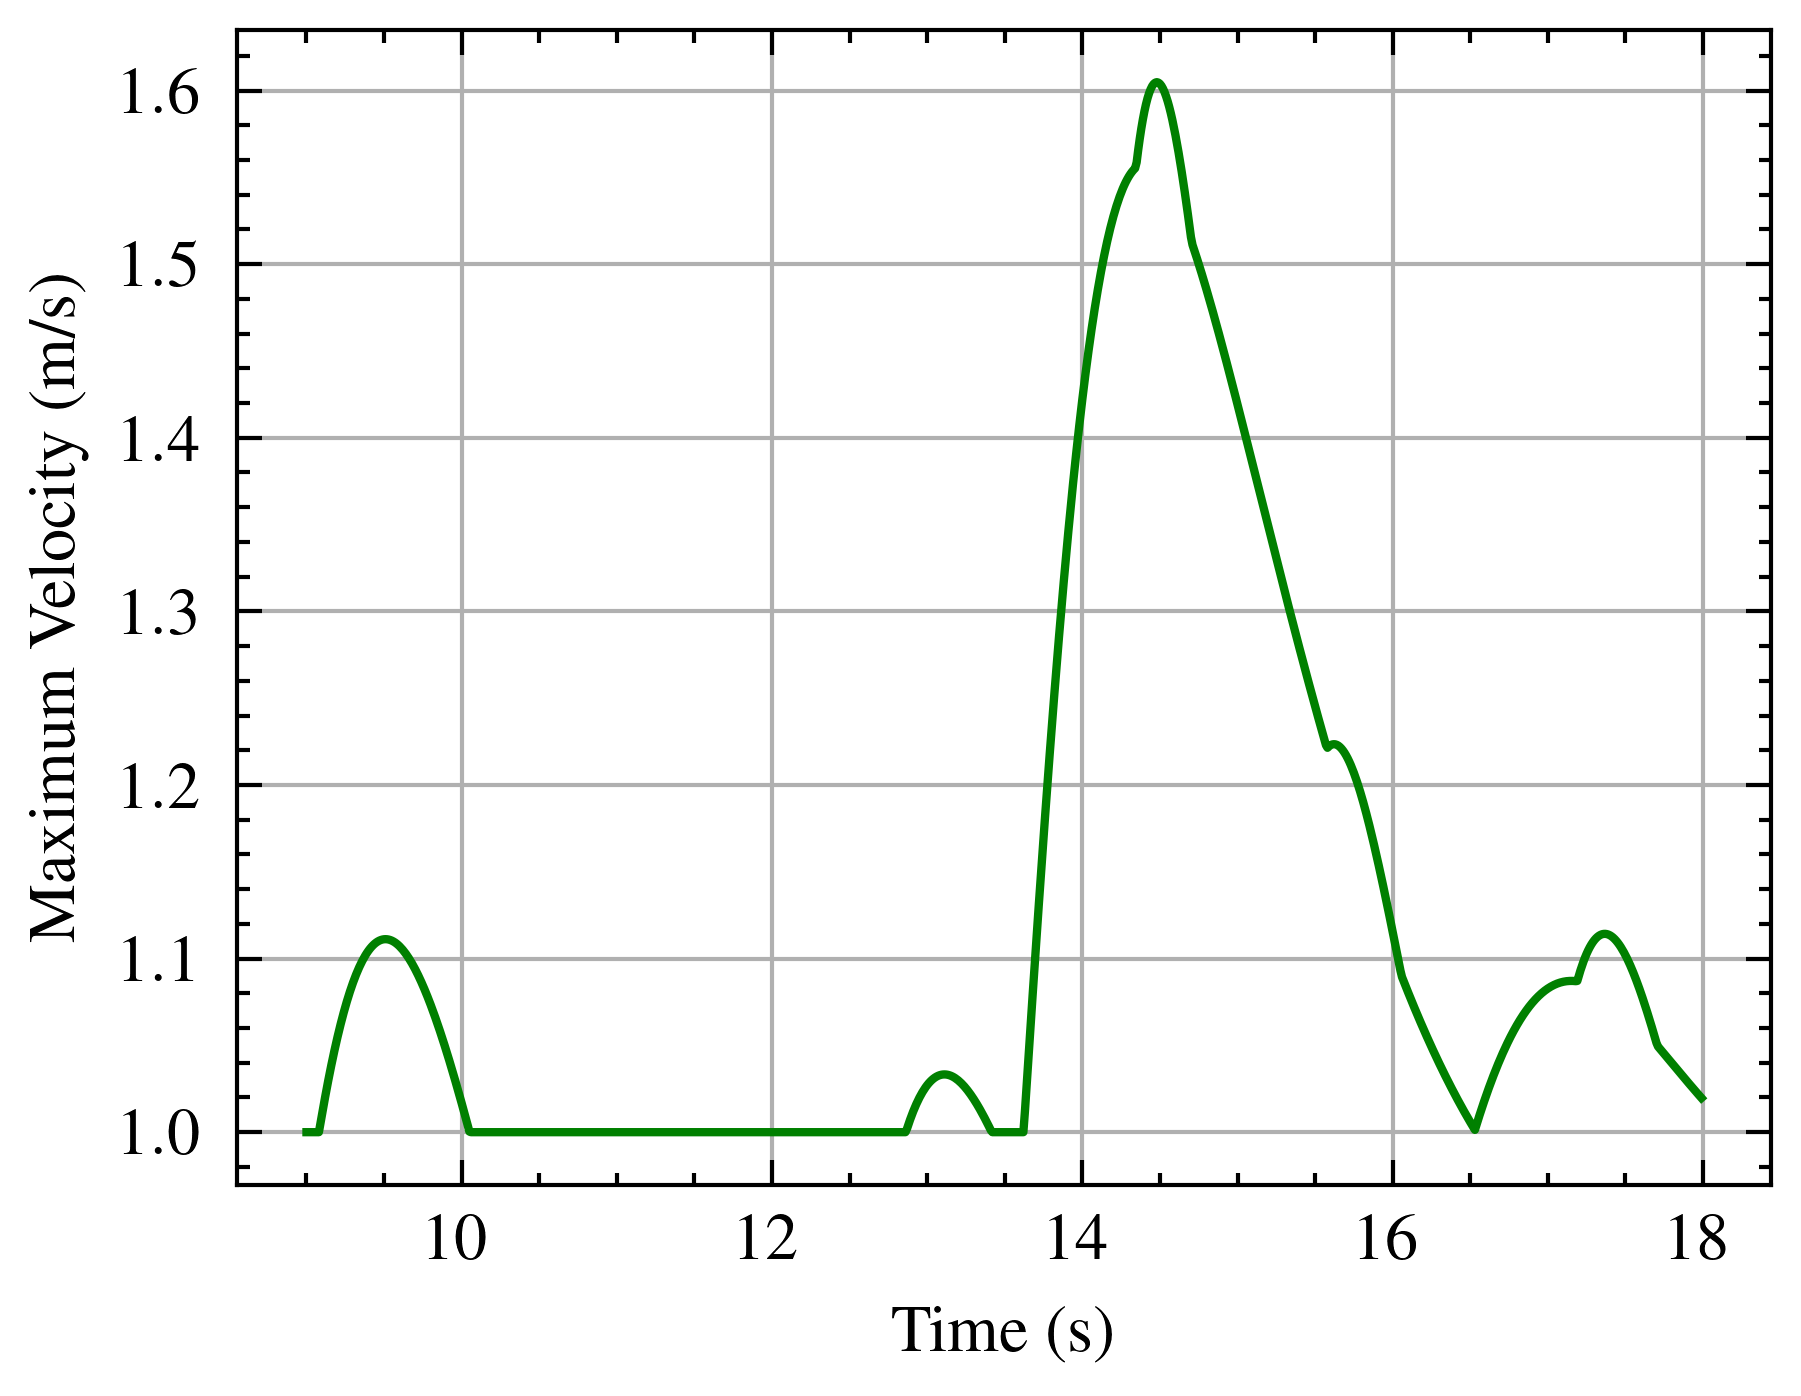
\includegraphics[width=0.5\textwidth]{image/Figure_5514.png}
			\caption{问题五最大速度关于时间的函数}
			\label{Figure_5514}
		\end{figure}
		
		可以发现,在目标区间 $t \in [9, 18]$ 内有多个局部极大值,且\textbf{难以确定是否存在更细粒度的局部极值点},因此采用启发式算法进行最大值求解。模拟退火算法是一种概率型全局优化算法,通过模拟系统温度逐渐降低时的随机搜索过程来寻找问题的全局最优解,适合用于多极大值时求解最大值。
		
		具体来说,模拟退火算法的迭代分为两步。首先,对于目标函数 $f(t)$ 和查找区域 $[l, r]$ 选定自变量的初始点 $t_i$ 后,模拟退火算法会随机选取范围内的一点 $t_{i+1}$ 。$t_{i+1}$ 的选取由下式决定。
		\begin{equation}
			t_{i+1} = t_i + random(-1, 1) \cdot T
		\end{equation}
		如果 $t{i+1}$ 的计算结果超出了求解范围边界,则可以在 $t_i$ 和边界之间随机选取一点作为 $t_{i+1}$ 。若 $v_{max}(t_1) \ge v_{max}(t_0)$,则将 $t_{i+1}$ 更新为 $t_1$ ;否则,将 $t_0$ 更新为 $t_1$ 的概率由 Metropolis 算法决定,即概率 $P$ 为:
		\begin{equation}
			P = \exp(-\dfrac{f(t_1) - f(t_0)}{T})
		\end{equation}
		
		对自变量进行了多次迭代更新后,将温度 $T$ 等比减小以模拟降低温度,即
		$$T_{i+1} = \alpha_t T_i$$
		随着温度的降低,自变量会更稳定地向最大值点收拢。取 $10^{-5}$ 作为最低温度。当温度 $T$ 下降至该温度后即停止迭代运算。
		
		模拟退火算法的相关代码在附录%
		的 sa.py 文件中给出了具体求解过程。
		
		取定初始值为 $T = 4$,$l=9.0$,$right=18.0$,$\alpha_t = 0.95$,$t_0 = \frac{l + r}{2} = 13.5$。经过降温 252 次迭代解得:当龙头速度为 $v_0 = 1$m/s 时,舞龙队的最大速度为 $v_m = 1.604793$m/s ,\textbf{在 14.480391s 时的第三、四、五、六、七节龙身的前把手处取得行进速度最大值。}多节把手速度完全相同的原因是第三、四、五、六节龙身均在半径为 $r1$ 的前一圆弧上
		
		依照题意,龙身各把手的最大速度不能超过 $v_{\text{把手}max} = 2$m/s ,因此满足题意的龙头的最大速度可以通过下式计算:
		$$ \dfrac{v_{\text{龙头}max}}{v_{\text{把手}max}} = \dfrac{v_0}{v_m} $$
		代入数据解得:
		\begin{equation}
			v_{\text{龙头}max} = 1.246267 \text{m/s}
		\end{equation}
		
		因此,\textbf{当龙头速度为 $v_{\text{龙头}max}= 1.246267$m/s 时,第三、四、五、六、七节把手在 14.480391s 处恰好达到速度最大值。并且能够保证在任一时间下各个把手的速度均不会超过 2m/s}
		
		
	%Part Six
	\section{模型的评价}
	\subsection{模型优点}
	\begin{enumerate}
		\item \textbf{建模过程完整可靠}。模型贴合实际,充分考虑了“板凳龙”的观赏性,同时通过约束条件保证了安全性。结合实际建立了微分方程、平面几何、解析几何、计算几何、单目标优化等多样模型,综合使用多种算法等方法求解。并对结果进行了数据分析和灵敏度分析,保证了过程的完整可靠性和模型求解的高效性。
		\item \textbf{可视化方法贯穿建模全程},提高了建模效率,更方便地对模型进行验证。通过对板凳龙运动过程的可视化,缩小了优化问题的范围;通过中间变量的可视化,有效分析了变量间的关系;通过对结果的可视化,方便地验证了结果的正确性和模型的可靠性。
		\item \textbf{合理使用启发式算法求解复杂优化问题}。借鉴粒子群算法,提出使用于求解本模型的拟粒子群算法,提高了模型的效率,并且更广泛的查找范围提高了模型的可信度;采用模拟退火算法对极值进行查找,有效解决了多峰函数难以确定极值的问题。
	\end{enumerate}

	\subsection{模型缺点}
	\begin{enumerate}
		\item 模型较为理想,未将板凳龙放置在三位空间中进行考虑,同时也忽略了举板凳的人对运动系统的影响,在现实中,模型可能需要进一步调整。
	\end{enumerate}

	
	%Part Seven
	\section{参考文献}
	\vspace{-2em} % 减小上面的间距
	\begin{thebibliography}{9}  
		\bibitem{ref1} 
		\bibitem{ref2} 
		\bibitem{ref3} 
		\bibitem{ref4}   
	\end{thebibliography}
	
	\newpage
	\section*{附录}
	
	附录1:支撑材料的文件列表
	
	
	
	附录2:初始化代码和数据处理代码
	
	main.py 用于指定运行求解各题目的函数。使用时对于每一题需单独运行相关代码,并注释掉无关代码。
	\begin{lstlisting}[language=python,columns=fullflexible,frame=shadowbox]
# main.py
from gen_xlsx import *
from sa import *
from cross import *
from trisection import *

import generate
import config

if __name__ == "__main__":
	print("请打开当前目录下的main.py文件,根据注释运行各问代码,查看输出结果")
	# 未运行倒数两个可视化代码会弹出仅有坐标系和时间标签的网页,请关闭后继续查看标准输出框的结果
	# 第一问数据生成
	# 初始时刻到 300s 为止,每秒整个舞龙队的位置,储存在当前目录下的result1_dis.xlsx中
	# dis_xlsx_init()
	# dis_fill_xlsx()
	
	# 初始时刻到 300s 为止,每秒整个舞龙队的速度,储存在当前目录下的result1_v.xlsx中
	# v_xlsx_init()
	# v_fill_xlsx()
	
	# 第二问数据生成
	# 舞龙队盘入恰好使得板凳之间不发生碰撞的时刻下舞龙队的位置和速度,储存在当前目录下的result2.xlsx中
	collision_xlsx_init()
	# time, if_in = pso_cal_min_distance(55)
	# print(f"在{time}s恰好发生碰撞")
	collision_fill_xlsx(412.4742127430167)
	
	# 第三问验证函数
	# print("问题三最小螺距:", cal_min_D())
	
	# 第四问数据生成
	# 以调头开始时间为零时刻,从 −100s 开始到 100s 为止,每秒舞龙队的位置,储存在当前目录下的result4_dis.xlsx中
	# q4_dis_xlsx_init()
	# q4_dis_fill()
	
	# 以调头开始时间为零时刻,从 −100s 开始到 100s 为止,每秒舞龙队的速度,储存在当前目录下的result4_v.xlsx中
	# q4_v_xlsx_init()
	# q4_v_fill()
	
	# 第五问验证算法
	# 模拟退火算法
	# sa()
	
	# 网页弹出后,网页部分内容为黑色,表明正在加载,请稍等片刻后,等待图像基本加载完毕,使用鼠标拖动边框或在可视化界面中滑动滚轮调节图像大小
	# 第一问可视化
	# generate.q1_generate_spiral()
	# generate.q1_generate(points, lines, bench_lines)
	
	# 第四问可视化
	# generate.q4_generate_curve()
	# generate.q4_generate(points, lines, bench_lines)
 	\end{lstlisting}
 	
 	config.py 文件为配置文件,用于存储计算精度要求、全局常量等参数信息
	\begin{lstlisting}[language=python,columns=fullflexible,frame=shadowbox]
# config.py
import time

import numpy as np

# 绘制等距螺线
# 参数设置
_spacing = 0.2  # 控制螺线显示效果
space = 55  # 控制螺距
len_head = 286  # 龙头长度
len_body = 165  # 龙身长度
section_num = 223  # 龙节数
theta_max = 32 * np.pi  # 控制螺线的最大角度
q4_start_time = -100
q4_end_time = 100

fixed_distances = [2 * _spacing * np.pi * len_head / space, 2 * _spacing * np.pi * len_body / space]   # 龙头前把手与后把手的间距 + 龙身与龙尾前把手与后把手的间距
actual_fixed_distances = [len_head, len_body]   # 龙头前把手与后把手的间距 + 龙身与龙尾前把手与后把手的间距
sys_length = 45
start_time = time.time()
actual_q4_start_time = time.time() + 100.0
actual_q4_end_time = time.time() - 100.0

dis_tolerance = 1e-12

##################################

# q4
median = 2.5
	
def set_spacing(space):
	global _spacing
	_spacing = space
	
	
	\end{lstlisting}
 	
 	gen\_xlsx.py 文件用于迭代计算舞龙队位置和速度并输出到xlsx文件中
	\begin{lstlisting}[language=python,columns=fullflexible,frame=shadowbox]
# gen_xlsx.py
from openpyxl import Workbook
from openpyxl.styles import Font
from calculate import *

import config

wb = Workbook()
ws = wb.active
font_new = Font(name='Times New Roman', size=10)
font_song = Font(name='宋体', size=10)

# q1填充行名
q1_dis_row_names = ["龙头x (m)", "龙头y (m)"]

for i in range(1, 222):
q1_dis_row_names.append(f"第{i}节龙身x (m)")
q1_dis_row_names.append(f"第{i}节龙身y (m)")

q1_dis_row_names.append("龙尾x (m)")
q1_dis_row_names.append("龙尾y (m)")
q1_dis_row_names.append("龙尾(后)x (m)")
q1_dis_row_names.append("龙尾(后)y (m)")

q1_v_row_names = ["龙头 (m/s)"]

for i in range(1, 222):
q1_v_row_names.append(f"第{i}节龙身  (m/s)")

q1_v_row_names.append("龙尾  (m/s)")
q1_v_row_names.append("龙尾(后) (m/s)")

# q1填充列名
q1_column_names = [f"{i} s" for i in range(301)]  # 从 0 s 到 21 s

# q2填充行名
q2_row_names = ["龙头"]

for i in range(1, 222):
q2_row_names.append(f"第{i}节龙身")

q2_row_names.append("龙尾")
q2_row_names.append("龙尾(后)")

# q2填充列名
q2_column_names = ["横坐标x (m)", "纵坐标y (m)", "速度 (m/s)"]

# q4_dis填充行名
q4_dis_row_names = q1_dis_row_names

# q4_dis填充列名
q4_dis_column_names = [f"{i} s" for i in range(-100, 101)]

# q4_v填充行名
q4_v_row_names = q1_v_row_names

# q4_v填充列名
q4_v_column_names = [f"{i} s" for i in range(-100, 101)]

def dis_xlsx_init():
for row_num, row_name in enumerate(q1_dis_row_names, start=2):
cell = ws.cell(row=row_num, column=1, value=row_name)
cell.font = font_new

for col_num, col_name in enumerate(q1_column_names, start=2):
cell = ws.cell(row=1, column=col_num, value=col_name)
cell.font = font_new


def dis_fill_xlsx():
	for time in range(301):
		theta = t_to_theta(time)
		pos = get_actual_position(theta, config.space)
		x = pos[0][0] / 100.0
		y = pos[1][0] / 100.0
		cell = ws.cell(row=2, column=time + 2, value=f"{x:.6f}")
		cell.font = font_new
		cell = ws.cell(row=3, column=time + 2, value=f"{y:.6f}")
		cell.font = font_new

		# 更新接下来的点的位置
		current_theta = theta
		for i in range(1, 224):
			delta_theta = find_actual_delta_theta(current_theta, config.actual_fixed_distances[0 if i == 1 else 1], config.space)
			current_theta += delta_theta
			pos = get_actual_position(current_theta, config.space)
			x = pos[0][0] / 100.0
			y = pos[1][0] / 100.0
			print(f"{time} {i}")
			cell = ws.cell(row=2 * (i + 1), column=time + 2, value=f"{x:.6f}")
			cell.font = font_new
			cell = ws.cell(row=2 * (i + 1) + 1, column=time + 2, value=f"{y:.6f}")
			cell.font = font_new

	wb.save("result1_dis.xlsx")


def v_xlsx_init():
	for row_num, row_name in enumerate(q1_v_row_names, start=2):
		cell = ws.cell(row=row_num, column=1, value=row_name)
		cell.font = font_new

	for col_num, col_name in enumerate(q1_column_names, start=2):
		cell = ws.cell(row=1, column=col_num, value=col_name)
		cell.font = font_new

def v_fill_xlsx():
	for time in range(301):
		dt = 1e-5
		theta = t_to_theta(time)
		pos = get_actual_position(theta, config.space)
		_theta = t_to_theta(time - dt)
		_pos = get_actual_position(_theta, config.space)
		ds = list_cartesian_distance(pos, _pos) / 100.0
		print(ds)
		v = ds / dt
		cell = ws.cell(row=2, column=time + 2, value=f"{v[0]:.6f}")
		cell.font = font_new

		# 更新接下来的点的位置
		current_theta = theta
		_current_theta = _theta
		for i in range(1, 224):
		delta_theta = find_actual_delta_theta(current_theta, config.actual_fixed_distances[0 if i == 1 else 1], config.space)
		current_theta += delta_theta
		pos = get_actual_position(current_theta, config.space)
		_delta_theta = find_actual_delta_theta(_current_theta, config.actual_fixed_distances[0 if i == 1 else 1], config.space)
		_current_theta += _delta_theta
		_pos = get_actual_position(_current_theta, config.space)
		ds = list_cartesian_distance(pos, _pos) / 100.0
		v = ds / dt
		print(time)
		cell = ws.cell(row=i + 2, column=time + 2, value=f"{v[0]:.6f}")
		cell.font = font_new
		
	wb.save("result1_v.xlsx")

def collision_xlsx_init():
	for row_num, row_name in enumerate(q2_row_names, start=2):
		cell = ws.cell(row=row_num, column=1, value=row_name)
		cell.font = font_song if row_num == 2 else font_new

	for col_num, col_name in enumerate(q2_column_names, start=2):
		cell = ws.cell(row=1, column=col_num, value=col_name)
		cell.font = font_new

def collision_fill_xlsx(t):
	time = t
	dt = 1e-5
	theta = t_to_theta(time)
	pos = get_actual_position(theta, config.space)
	x = pos[0][0] / 100.0
	y = pos[1][0] / 100.0
	print(x, y)
	cell = ws.cell(row=2, column=2, value=f"{x:.6f}")
	cell.font = font_new
	cell = ws.cell(row=2, column=3, value=f"{y:.6f}")
	cell.font = font_new
	_theta = t_to_theta(time - dt)
	_pos = get_actual_position(_theta, config.space)
	ds = list_cartesian_distance(pos, _pos) / 100.0
	v = ds / dt
	cell = ws.cell(row=2, column=4, value=f"{v[0]:.6f}")
	cell.font = font_new

	# 更新接下来的点的位置
	current_theta = theta
	_current_theta = _theta
	for i in range(1, 224):
		delta_theta = find_actual_delta_theta(current_theta, config.actual_fixed_distances[0 if i == 1 else 1],
		config.space)
		current_theta += delta_theta
		pos = get_actual_position(current_theta, config.space)
		x = pos[0][0] / 100.0
		y = pos[1][0] / 100.0
		print(x, y)
		cell = ws.cell(row=i + 2, column=2, value=f"{x:.6f}")
		cell.font = font_new
		cell = ws.cell(row=i + 2, column=3, value=f"{y:.6f}")
		cell.font = font_new
		_delta_theta = find_actual_delta_theta(_current_theta, config.actual_fixed_distances[0 if i == 1 else 1],
		config.space)
		_current_theta += _delta_theta
		_pos = get_actual_position(_current_theta, config.space)
		ds = list_cartesian_distance(pos, _pos) / 100.0
		v = ds / dt
		cell = ws.cell(row=i + 2, column=4, value=f"{v[0]:.6f}")
		cell.font = font_new
		
	wb.save("result2.xlsx")

def q4_dis_xlsx_init():
	for row_num, row_name in enumerate(q4_dis_row_names, start=2):
	cell = ws.cell(row=row_num, column=1, value=row_name)
	cell.font = font_song if row_num == 2 else font_new
	
	for col_num, col_name in enumerate(q4_dis_column_names, start=2):
	cell = ws.cell(row=1, column=col_num, value=col_name)
	cell.font = font_new

def q4_dis_fill():
	dis_tolerance = 1e-12
	for time in range(-100, 101):
		# 更新第一个点的位置
		x, y = t_to_xy_q4(time)
		cell = ws.cell(row=2, column=time + 102, value=f"{x:.6f}")
		cell.font = font_new
		cell = ws.cell(row=3, column=time + 102, value=f"{y:.6f}")
		cell.font = font_new

		ergodic_time = time
		for i in range(1, 224):
			delta_time = find_delta_time(ergodic_time, config.actual_fixed_distances[0 if i == 1 else 1], dis_tolerance)
			ergodic_time -= delta_time
			_x, _y = t_to_xy_q4(ergodic_time)
			cell = ws.cell(row=2 * (i + 1), column=time + 102, value=f"{_x:.6f}")
			cell.font = font_new
			cell = ws.cell(row=2 * (i + 1) + 1, column=time + 102, value=f"{_y:.6f}")
			cell.font = font_new

		print(time)

	wb.save("result4_dis.xlsx")

def q4_v_xlsx_init():
	for row_num, row_name in enumerate(q4_v_row_names, start=2):
	cell = ws.cell(row=row_num, column=1, value=row_name)
	cell.font = font_song if row_num == 2 else font_new
	
	for col_num, col_name in enumerate(q4_v_column_names, start=2):
	cell = ws.cell(row=1, column=col_num, value=col_name)
	cell.font = font_new

def q4_v_fill():
	dis_tolerance = 1e-12
	for time in range(-100, 101):
		dt = 1e-5
		x, y = t_to_xy_q4(time)
		_x, _y = t_to_xy_q4(time - dt)
		ds = list_cartesian_distance([x, y], [_x, _y])
		v = ds / dt
		cell = ws.cell(row=2, column=time + 102, value=f"{v:.6f}")
		cell.font = font_new
		
		# 更新接下来的点的位置
		ergodic_time = time
		_ergodic_time = time - dt
		for i in range(1, 224):
			delta_time = find_delta_time(ergodic_time, config.actual_fixed_distances[0 if i == 1 else 1], dis_tolerance)
			ergodic_time -= delta_time
			x, y = t_to_xy_q4(ergodic_time)
			_delta_time = find_delta_time(_ergodic_time, config.actual_fixed_distances[0 if i == 1 else 1], dis_tolerance)
			_ergodic_time -= _delta_time
			_x, _y = t_to_xy_q4(_ergodic_time)
			ds = list_cartesian_distance([x, y], [_x, _y])
			# print(i, ds)
			v = ds / dt
			cell = ws.cell(row=i + 2, column=time + 102, value=f"{v:.6f}")
			cell.font = font_new
	
		print(time)
	
	wb.save("result4_v.xlsx")

def q4_v_fill_test():
	dis_tolerance = 1e-12
	col = 1
	time = 381
	end_time = 384
	while time < end_time:
		dt = 1e-5
		x, y = t_to_xy_q4(time)
		_x, _y = t_to_xy_q4(time - dt)
		ds = list_cartesian_distance([x, y], [_x, _y])
		v = ds / dt
		cell = ws.cell(row=2, column=col, value=f"{v:.6f}")
		cell.font = font_new
	
		# 更新接下来的点的位置
		ergodic_time = time
		_ergodic_time = time - dt
		for i in range(1, 224):
			delta_time = find_delta_time(ergodic_time, config.actual_fixed_distances[0 if i == 1 else 1], dis_tolerance)
			ergodic_time -= delta_time
			x, y = t_to_xy_q4(ergodic_time)
			_delta_time = find_delta_time(_ergodic_time, config.actual_fixed_distances[0 if i == 1 else 1], dis_tolerance)
			_ergodic_time -= _delta_time
			_x, _y = t_to_xy_q4(_ergodic_time)
			ds = list_cartesian_distance([x, y], [_x, _y])
			v = ds / dt
			cell = ws.cell(row=i + 2, column=col, value=f"{v:.6f}")
			cell.font = font_new
			
		col += 1
		time += 0.2
		print(time)
	
	wb.save("result4_v_t.xlsx")

def q5_v_find_test():
	dis_tolerance = 1e-12
	col=1
	time: float = 14.45
	cell = ws.cell(row=1, column=1, value="时间 (s)")
	while (time < 14.55):
		time += 0.0001
		col += 1
		dt = 1e-5
		x, y = t_to_xy_q4(time)
		_x, _y = t_to_xy_q4(time - dt)
		ds = list_cartesian_distance([x, y], [_x, _y])
		v = ds / dt
		cell = ws.cell(row=1, column=col, value=time)
		cell = ws.cell(row=2, column=col, value=f"{v:.6f}")
		cell.font = font_new
		
		# 更新接下来的点的位置
		ergodic_time = time
		_ergodic_time = time - dt
		for i in range(1, 11):
			delta_time = find_delta_time(ergodic_time, config.actual_fixed_distances[0 if i == 1 else 1], dis_tolerance)
			ergodic_time -= delta_time
			x, y = t_to_xy_q4(ergodic_time)
			_delta_time = find_delta_time(_ergodic_time, config.actual_fixed_distances[0 if i == 1 else 1], dis_tolerance)
			_ergodic_time -= _delta_time
			_x, _y = t_to_xy_q4(_ergodic_time)
			ds = list_cartesian_distance([x, y], [_x, _y])
			v = ds / dt
			cell = ws.cell(row=i + 2, column=col, value=f"{v:.6f}")
			cell.font = font_new
	
		print("calculating:", time)
	
	wb.save("result5_v_test.xlsx")

	\end{lstlisting}
 	
	calculate.py 文件存放基础计算方法,如二分查找,极坐标距离等公式
	\begin{lstlisting}[language=python,columns=fullflexible,frame=shadowbox]
# calculate.py
from vpython import *
from q4 import *
from scipy.optimize import fsolve

import math
import numpy as np
import config

# 函数
# 根据theta计算螺线上点的位置
def get_position(theta):
    r = config._spacing * theta
    x = r * np.cos(theta)
    y = r * np.sin(theta)
    return vector(x, y, 0)

# 计算两点之间的距离
def cartesian_distance(pos1, pos2):
    return np.sqrt((pos1.x - pos2.x) ** 2 + (pos1.y - pos2.y) ** 2)

# 优化
def polar_distance(theta_1, theta_2):
    rho_1 = config._spacing * theta_1
    rho_2 = config._spacing * theta_2
    return np.sqrt(rho_1 ** 2 + rho_2 ** 2 - 2 * rho_1 * rho_2 * np.cos(theta_1 - theta_2))

# 使用二分法寻找更准确的 delta_theta
def find_delta_theta(theta, fixed_distance, dis_tolerance):
    # 二分上下限
    low = 0
    high = np.pi - 1e-2
    while high - low > dis_tolerance:
        mid = (low + high) / 2
        pos1 = get_position(theta)
        pos2 = get_position(theta + mid)
        dist = cartesian_distance(pos1, pos2)
        # dist = polar_distance(theta, theta + mid)
        if dist < fixed_distance:
            low = mid
        else:
            high = mid
    return (low + high) / 2

def find_delta_time(time, fixed_distance, dis_tolerance):
    low = 1.5
    high = 6
    while high - low > dis_tolerance:
        mid = (low + high) / 2
        x1, y1 = t_to_xy_q4(time)
        x2, y2 = t_to_xy_q4(time - mid)
        x1, y1 = x1 * 100, y1 * 100
        x2, y2 = x2 * 100, y2 * 100
        dist = list_cartesian_distance([x1, y1], [x2, y2])
        # dist = polar_distance(theta, theta + mid)
        if dist < fixed_distance:
            low = mid
        else:
            high = mid
    return (low + high) / 2

def list_cartesian_distance(pos1, pos2):
    return np.sqrt((pos1[0] - pos2[0]) ** 2 + (pos1[1] - pos2[1]) ** 2)

def get_actual_position(theta, space):
    r = config._spacing * theta
    x = r * np.cos(theta) / (2 * config._spacing * np.pi) * space
    y = r * np.sin(theta) / (2 * config._spacing * np.pi) * space
    return [x, y]

def find_actual_delta_theta(theta, fixed_distance, space):
    # 二分上下限
    low = 0
    high = 4
    while high - low > config.dis_tolerance:
        mid = (low + high) / 2
        pos1 = get_actual_position(theta, space)
        pos2 = get_actual_position(theta + mid, space)
        dist = list_cartesian_distance(pos1, pos2)
        # dist = polar_distance(theta, theta + mid)
        if dist < fixed_distance:
            low = mid
        else:
            high = mid
    return (low + high) / 2

# 需要已知的参数 t 来求解 theta
def theta_t(theta):
    return -1/2 * np.log(np.sqrt(1 + theta**2) - theta) + 1/2 * theta * np.sqrt(theta ** 2 + 1)

D_q1 = 0.55 # 螺距 m
v_q1 = 1 # 龙头速度 m/s
C_q1 = theta_t(32 * math.pi) * D_q1 / (2*math.pi) # 积分常数,不要动

def equ(theta, t, D, v, C):
    return - theta_t(theta) * D / (2 * math.pi) - v * t + C

def t_to_theta(t, D=D_q1, v=v_q1, C=C_q1):
    initial = 0.0
    return fsolve(equ, initial, args=(t, D, v, C))

def t_to_dis(t, space):
    positions = np.empty((224, 2))
    theta = t_to_theta(t)
    pos = get_actual_position(theta, space)
    x = pos[0][0] / 100.0
    y = pos[1][0] / 100.0
    positions[0] = np.array([x, y])

    current_theta = theta
    for i in range(1, 224):
        delta_theta = find_actual_delta_theta(current_theta, config.actual_fixed_distances[0 if i == 1 else 1], space)
        current_theta += delta_theta
        pos = get_actual_position(current_theta, space)
        x = pos[0][0] / 100.0
        y = pos[1][0] / 100.0
        positions[i] = np.array([x, y])

    return positions
	\end{lstlisting}
 	
	q4.py 文件存储着和第四题第五题有关的函数
	\begin{lstlisting}[language=python,columns=fullflexible,frame=shadowbox]
# q4.py
import numpy as np
import matplotlib.pyplot as plt
from scipy.optimize import fsolve
import math

R = 4.5 # m
D_q4 = 1.7 # 螺距 m
v_q4 = 1 # 龙头速度 m/s

theta0 = 2 * np.pi * R / D_q4
# print(f"theta0 = {theta0 / (np.pi)} * pi")
# print(f"theta0 = {theta0}")
# print(f"theta0 + pi = {theta0 + np.pi}")
k = (np.sin(theta0) + theta0 * np.cos(theta0)) / (np.cos(theta0) - theta0 * np.sin(theta0))
# print(f"k = {k}")

x0 = R * np.cos(theta0)
y0 = R * np.sin(theta0)

x0_ = -x0
y0_ = -y0

# print(f"(x0, y0) = ({x0}, {y0})")

A = np.array([[R * np.cos(theta0), R * np.sin(theta0)],
				[1, k]])

b = np.array([0, k * R * np.sin(theta0) + R * np.cos(theta0)])

x3, y3 = np.linalg.solve(A, b)

# print(f"(x3, y3) = ({x3}, {y3})")

x1 = 1.0 / 3.0 * x0 + 2.0 / 3.0 * x3
y1 = 1.0 / 3.0 * y0 + 2.0 / 3.0 * y3

# print(f"(x1, y1) = ({x1}, {y1})")

x2 = - x0 + (x1 - x3)
y2 = - y0 + (y1 - y3)

# print(f"(x2, y2) = ({x2}, {y2})")

r2 = np.sqrt((x1 - x3) ** 2 + (y1 - y3) ** 2)
r1 = 2 * r2

# print(f"r2 = {r2}, r1 = {r1}")

xt = 2.0 / 3.0 * x2 + 1.0 / 3.0 * x1
yt = 2.0 / 3.0 * y2 + 1.0 / 3.0 * y1

# print(f"tangent_point = ({xt}, {yt})")

def arctan3(y, x):
	ret0 = np.arctan2(y, x)
	if ret0 < 0:
		return ret0 + 2 * np.pi
	else:
		return ret0

theta_11 = arctan3(yt - y1, xt - x1)
theta_12 = arctan3(y0 - y1, x0 - x1)
	
theta_21 = np.arctan2(yt - y2, xt - x2)
theta_22 = np.arctan2(y0_ - y2, x0_ - x2)

w1 = v_q4 / r1 # 第二段圆弧的角速度
w2 = v_q4 / r2 # 第一段圆弧的角速度
t1 = (theta_12 - theta_11) / w1 # 离开第一段圆弧的时刻
t2 = t1 + (theta_22 - theta_21) / w2 # 离开第二段圆弧的时刻
# print(f"t1={t1}, t2={t2}")

def theta_t_q4(theta):
	return -1/2 * np.log(np.sqrt(1 + theta**2) - theta) + 1/2 * theta * np.sqrt(theta ** 2 + 1)

C_q4_0 = theta_t_q4(theta0) * D_q4 / (2*math.pi) # 积分常数,不要动
C_q4_3 = - theta_t_q4(theta0) * D_q4 / (2*math.pi) + v_q4 * t2

def equ_q4_0(theta, t):
	return - theta_t_q4(theta) * D_q4 / (2 * math.pi) - v_q4 * t + C_q4_0

def equ_q4_3(theta, t):
	return theta_t_q4(theta - np.pi) * D_q4 / (2 * math.pi) - v_q4 * t + C_q4_3

def rho_q4_0(theta): # 极坐标进入路线方程
	return D_q4 / (2 * np.pi) * theta

def rho_q4_3(theta) :
	return D_q4 / (2 * np.pi) * (theta - np.pi)

def t_to_theta_q4_0(t):
	initial = 0.0
	return fsolve(equ_q4_0, initial, args=(t))

def t_to_theta_q4_1(t):
	x = x1 + r1 * np.cos(theta_12 - w1 * t) # 顺时针旋转,角速度为负
	y = y1 + r1 * np.sin(theta_12 - w1 * t)
	return x, y

def t_to_theta_q4_2(t):
	x = x2 + r2 * np.cos(theta_21 + w2 * (t - t1))
	y = y2 + r2 * np.sin(theta_21 + w2 * (t - t1))
	return x, y

def t_to_theta_q4_3(t):
	initial = 0.0
	return fsolve(equ_q4_3, initial, args=(t))

def t_to_xy_q4(t):
	if t < 0 :
		angle = t_to_theta_q4_0(t)
		rho = rho_q4_0(angle)
		x = rho * np.cos(angle)
		y = rho * np.sin(angle)
		return float(x), float(y)
	elif t < t1:
		return t_to_theta_q4_1(t)
	elif t < t2:
		return t_to_theta_q4_2(t)
	else:
		angle = t_to_theta_q4_3(t)
		rho = rho_q4_3(angle)
		x = rho * np.cos(angle)
		y = rho * np.sin(angle)
		return float(x), float(y)

# print(t_to_xy_q4(-0.1))

# plt.style.use(['science'])
# plt.rcParams['font.family'] = 'Microsoft YaHei'

# # 定义等距螺线的角度范围
# theta_spiral = np.linspace(theta0, 8 * np.pi, 1000)
# rho_spiral = (1.7 / (2 * np.pi)) * theta_spiral
# x_spiral = rho_spiral * np.cos(theta_spiral)
# y_spiral = rho_spiral * np.sin(theta_spiral)

# theta_spiral_ = np.linspace(theta0 - np.pi, 7 * np.pi, 1000)
# rho_spiral_ = (1.7 / (2 * np.pi)) * (theta_spiral_ + np.pi)
# x_spiral_ = rho_spiral_ * np.cos(theta_spiral_)
# y_spiral_ = rho_spiral_ * np.sin(theta_spiral_)

# # 圆的半径
# r = 4.5
# theta_circle = np.linspace(0, 2 * np.pi, 100)
# x_circle = r * np.cos(theta_circle)
# y_circle = r * np.sin(theta_circle)

# # 圆心的半径
# theta_circle1 = np.linspace(theta_21, theta_22, 1000)
# x_circle1 = (r2 * np.cos(theta_circle1)) + x2
# y_circle1 = (r2 * np.sin(theta_circle1)) + y2
# theta_circle2 = np.linspace(theta_11, theta_12, 1000)
# x_circle2 = (r1 * np.cos(theta_circle2)) + x1
# y_circle2 = (r1 * np.sin(theta_circle2)) + y1

# # 创建图形和坐标轴
# fig, ax = plt.subplots()

# # 绘制等距螺线
# ax.plot(x_spiral, y_spiral, 'b', label='盘入螺线')
# ax.plot(x_spiral_, y_spiral_, 'g', label='盘出螺线')

# # 绘制以原点为中心的圆
# ax.plot(x_circle, y_circle, 'r', label='掉头区域')

# # 绘制以(x1, y1)为圆心的圆
# ax.plot(x_circle1, y_circle1, 'orange', label='前一圆弧')
# ax.plot(x_circle2, y_circle2, 'orange', label='后一圆弧')

# # 绘制两个点
# # ax.scatter([x3, x1], [y3, y1], color=['green', 'purple'], s=100, label=['Point (x3, y3)', 'Point (x1, y1)'])
# # ax.scatter([xt], [yt], color=['green'], s=10, label=['(xt, yt)'])
# # ax.scatter([x1], [y1], color=['green'], s=10, label=['(x1, y1)'])
# # ax.scatter([x2], [y2], color=['green'], s=10, label=['(x2, y2)'])
# for dt in range(-100, 100, 1):
#     x, y = t_to_xy_q4(dt)
#     # print(f"x = {x}, y = {y}")
#     ax.scatter([x], [y], s=10, color = ["purple"])
# # ax.plot([x1, xt], [y1, yt], color='purple')
# # ax.plot([x1, x0], [y1, y0], color='purple')
# # ax.plot([x2, xt], [y2, yt], color='purple')
# # ax.plot([x2, x0_], [y2, y0_], color='purple')

# # 添加图例
# # ax.legend()

# # 设置图表标题和显示图形
# ax.set_title('问题四行进曲线')
# ax.set_xlabel('X 坐标')
# ax.set_ylabel('Y 坐标')

# ax.set_aspect('equal')

# plt.grid(True)
# plt.show()
	\end{lstlisting}
 	
	\begin{lstlisting}[language=python,columns=fullflexible,frame=shadowbox]
	\end{lstlisting}
 	
 cross.py 用于处理所有与板凳碰撞有关的问题
	\begin{lstlisting}[language=python,columns=fullflexible,frame=shadowbox]
# cross.py
import random

import numpy as np
from astropy.modeling.functional_models import Box1D
from joblib.testing import param
from mpmath.math2 import sqrt2
from numpy.matrixlib.defmatrix import matrix
from pandas.core.indexes.multi import sparsify_labels
from statsmodels.tsa.statespace.simulation_smoother import check_random_state
from openpyxl import load_workbook
from sympy.abc import epsilon

import config
from calculate import t_to_dis
from calculate import t_to_theta

# 1.以下函数由板凳的两个把手直角坐标计算板凳的四个端点直角坐标
# 2 dot -> 4 edge
lambda_of_head = 27.5 / 286
lambda_of_not_head = 27.5 / 165
lambda_move_head = 15 / 286
lambda_move_not_head = 15 / 165
def cal_long_side(front_dot, back_dot, head):
    back_front_vector = front_dot - back_dot
    if head:
        front_end = np.array([(lambda_of_head + 1) * front_dot[0] - lambda_of_head * back_dot[0],
                              (lambda_of_head + 1) * front_dot[1] - lambda_of_head * back_dot[1]])
        back_end  = np.array([(lambda_of_head + 1) * back_dot[0] - lambda_of_head * front_dot[0],
                              (lambda_of_head + 1) * back_dot[1] - lambda_of_head * front_dot[1]])
        move_vector = np.array([back_front_vector[1] * lambda_move_head, - back_front_vector[0] * lambda_move_head])
    else :
        front_end = np.array([(lambda_of_not_head + 1) * front_dot[0] - lambda_of_not_head * back_dot[0],
                              (lambda_of_not_head + 1) * front_dot[1] - lambda_of_not_head * back_dot[1]])
        back_end  = np.array([(lambda_of_not_head + 1) * back_dot[0] - lambda_of_not_head * front_dot[0],
                              (lambda_of_not_head + 1) * back_dot[1] - lambda_of_not_head * front_dot[1]])
        move_vector = np.array([back_front_vector[1] * lambda_move_not_head, - back_front_vector[0] * lambda_move_not_head])
    # print(front_end + move_vector, back_end + move_vector, front_end - move_vector, back_end - move_vector)
    return front_end + move_vector, back_end + move_vector, front_end - move_vector, back_end - move_vector

# cal_long_side(np.array([0,0]), np.array([165 * sqrt2 / 2, 165 * sqrt2 / 2]), False)

#2.以下函数通过跨立实验检测两线段是否相交
# return true if 2 edges cross
def cross_test(edge1, edge2):
    A0 = edge1[0]
    A1 = edge1[1]
    B0 = edge2[0]
    B1 = edge2[1]

    A0B0 = B0 - A0
    A0B1 = B1 - A0
    A0A1 = A1 - A0

    vector1 = np.cross(A0A1, A0B0)
    vector2 = np.cross(A0A1, A0B1)

    B0A0 = -A0B0
    B0A1 = A1 - B0
    B0B1 = B1 - B0

    vector3 = np.cross(B0B1, B0A0)
    vector4 = np.cross(B0B1, B0A1)

    #print(vector1, vector2)
    #print(vector3, vector4)
    if vector1 * vector2 <= 0 and vector3 * vector4 <= 0:
        print(f'crossed edges:\n1:{edge1},\n2:{edge2}')
        #print(vector1, vector2, vector3, vector4)
    return vector1 * vector2 <= 0 and vector3 * vector4 <= 0

#print(cross_test(np.array([[0,0],[1,0]]),np.array([[0,-1],[0.000,0.3]])))

# 3.给定全体把手位置张量,判断全域有无板凳碰撞
def all_cross_check(dot_matrix):
    edge_list = []
    for i in range(dot_matrix.shape[0] - 1):
        A0, A1, B0, B1 = cal_long_side(dot_matrix[i], dot_matrix[i + 1], i == 0)
        edge_list.append(np.array([A0, A1])) # even:inside
        edge_list.append(np.array([B0, B1])) # odd: outside

    cross = False
    for i in range(2, len(edge_list), 2):
        for j in range(i - 3, 0, -2):
            #print(i, j)
            if cross_test(edge_list[i], edge_list[j]):
                print(f'crossed benches:{i // 2}, {j // 2}')
                cross = True
                break
        if cross:
            break

    return cross

# 4.以下两个辅助函数
def cal_nearest(space):
    #print(t_to_dis(0, space))
    delta = 10
    crash = 280
    epsilon = 0.01
    while delta >= epsilon:
        low = 230
        high = crash
        time = low
        while time < high:
            time = time + delta
            matrix = t_to_dis(time, space)
            print(time)
            #print(all_cross_check(matrix))
            if all_cross_check(matrix):
                crash = time if time < crash else crash
                break
        delta /= 10
    print(crash)

#cal_nearest(45)

def local_check():
    for t in range(40950, 41200, 5):
        time = t / 100
        matrix = t_to_dis(time, 55)
        #print(t_to_dis(time))
        print(time)
        print(all_cross_check(matrix))

#local_check()

# 5.下面的函数用拟粒子群算法计算一定螺距下板凳龙前进的最长时间以及龙头前把手与原点的最近距离
max = 30
w = 0.5
c1 = 0.5
c2 = 1
max_time = 500
def pso_cal_min_distance(space, n = 10, c1 = 0.5, c2 = 1):
    partical = []
    partical_v = []
    pbest    = []
    gbest    = (max_time, True)
    can_enter = True

    for i in range(n):
        print(f'initial:{i}/{n}')
        partical.append(random.random() * max_time)
        partical_v.append(random.random())
        pbest.append((partical[i], all_cross_check(t_to_dis(partical[i], space))))
        if pbest[i][0] < gbest[0] and pbest[i][1]:
            gbest = pbest[i]

    for j in range(max):
        for i in range(n):
            partical_v[i] = w * partical_v[i] + c1 * random.random() * (
                        pbest[i][0] - partical[i]) + c2 * random.random() * (gbest[0] - partical[i])
            partical[i] = partical[i] + partical_v[i]

            if partical[i] > 500:
                partical[i] = 500
            if partical[i] < 0:
                partical[i] = 0

            cross = all_cross_check(t_to_dis(partical[i], space))
            if not pbest[i][1] and cross:
                pbest[i] = (partical[i], True)

            elif pbest[i][1] and cross:
                pbest[i] = pbest[i] if pbest[i][0] < partical[i] else (partical[i], cross)

            if pbest[i][0] < gbest[0] and pbest[i][1]:
                gbest = pbest[i]

            if pbest[i][0] > gbest[0]:
                partical[i] = gbest[0] * random.random()
                pbest[i] = partical[i], all_cross_check(t_to_dis(partical[i], space)) # if not best, go to a random smaller position

            # print(f'{i}, {pbest[i]}, {gbest}')
            # print(f'{space}, {t_to_theta(gbest[0], D=space / 100) / 2 / np.pi * space}')

    return gbest[0], t_to_theta(gbest[0], D=space / 100) / 2 / np.pi * space > 450 # can enter

#print(pso_cal_min_distance(55, 10, c1, c2))

smallest = 46
biggist  = 50

# for i in range(smallest, biggist + 1, 1):
#     pso_cal_min_distance(i, 10, c1, c2)
#     pso_cal_min_distance(i + 0.5, 10, c1, c2)
#
# smallest = 545
# biggist  = 555
#
# for i in range(smallest, biggist + 1, 1):
#     pso_cal_min_distance(i / 10, 10, c1, c2)

# pso_cal_min_distance(55, 10, c1, c2)
#

# 6.二分查找求最短螺距
def cal_min_D():
    smallest = 45
    biggist  = 46
    space = (biggist + smallest) / 2
    for i in range(1):
        print(space)
        if pso_cal_min_distance(space, 10, c1, c2)[1]:
            biggist = space
        else :
            smallest = space
        space = (biggist + smallest) / 2

    return space

# cal_min_D()

	\end{lstlisting}
 	
	sa.py 文件用于存储和第五题模拟退火算法有关的函数和变量
	\begin{lstlisting}[language=python,columns=fullflexible,frame=shadowbox]
# sa.py
import numpy as np
import random as rd
import math

import config
from q4 import t_to_xy_q4
from calculate import find_delta_time, list_cartesian_distance

right =18.0
left  =9.0
alpha =0.95
T     =4.0
initial_t = (right + left) / 2
iteration = 5 # 每个温度下迭代次数
node_num = 10 # 默认只计算前十节的最大速度以加快计算

def next_time(x):
    x_next = x + T * 2 * (rd.random()-0.5)
    if x_next < left:
        temp = rd.random()
        return temp*left+(1-temp)*x
    elif x_next > left and x_next <= right:
        return x_next
    else:
        temp = rd.random()
        return temp*right+(1-temp)*x


def evaluate_function(t, dt=1e-5, node_num=node_num):
    # print(f"maximum velocity at {t:.6f}s is...", end='')
    dis_tolerance = 1e-12
    vmax = 0
    index_max: int
    
    x, y = t_to_xy_q4(t)
    _x, _y = t_to_xy_q4(t - dt)
    ds = list_cartesian_distance([x, y], [_x, _y])
    v = ds / dt
    
    if v > vmax:
        vmax = v
        index_max = 0

    # 更新接下来的点的位置
    ergodic_time = t
    _ergodic_time = t - dt
    for i in range(1, 11):
        delta_time = find_delta_time(ergodic_time, config.actual_fixed_distances[0 if i == 1 else 1], dis_tolerance)
        ergodic_time -= delta_time
        x, y = t_to_xy_q4(ergodic_time)
        _delta_time = find_delta_time(_ergodic_time, config.actual_fixed_distances[0 if i == 1 else 1], dis_tolerance)
        _ergodic_time -= _delta_time
        _x, _y = t_to_xy_q4(_ergodic_time)
        ds = list_cartesian_distance([x, y], [_x, _y])
        v = ds / dt
    
        if v > vmax:
            vmax = v
            index_max = i
    # print(f"{vmax:.6f}m/s")
    return vmax, i


# 使用 Metropolis 算法计算概率
def p(t, t_next):
    return math.exp(-abs(evaluate_function(t)[0]-evaluate_function(t_next)[0])/(T * 0.01))

def sa():
    global T
    time_tolerance = 1e-5
    rd.seed(1234)
    t = initial_t
    iter = 0
    total_iter = int(np.log(time_tolerance / T) / np.log(alpha))
    f_t, index_t = evaluate_function(t)
    print(index_t.__class__)
    f_next: float
    while T > time_tolerance:
        iter += 1
        print(f"\033[32mRound ({iter}/{total_iter}): {f_t:.6f}m/s at {t:.6f}s when T={T:.06f}\033[0m")
        for i in range(iteration):
            t_next = next_time(t)
            f_t, index_t = evaluate_function(t)
            f_next, index_next = evaluate_function(t_next)
            if f_next >= f_t:
                print(f"{f_next:.6f}m/s at {t_next:.06f}s is faster and accpected")
                t = t_next
                index_t = index_next
            elif rd.random() <= p(t, t_next):
                print(f"{f_next:.6f}m/s at {t_next:.06f}s is ramdomly accepted")
                t = t_next
                index_t = index_next
        T *= alpha
    print(f'最大值为:{evaluate_function(t)[0]:.6f}m/s, 最大值点为:{t}s, 把手号为:{index_t}')

	\end{lstlisting}
\end{document}